%----------------------------------------------------------------
%
%  File    :  thesis.tex
%
%  Author  :  Keith Andrews, ISDS, TU Graz, Austria
%
%  Created :  30 Jul 1997
% 
%  Changed :  22 Jan 2021
%
%----------------------------------------------------------------

\documentclass[11pt]{book}

\usepackage[
  a4paper,
  twoside,
  top=5mm,                % top margin
  bottom=7mm,             % bottom margin
  inner=20mm,             % inner margin (next to binding)
  outer=20mm,             % outer margin (opposite binding)
  bindingoffset=10mm,     % on binding side
  includeheadfoot,        % include head(er) and foot(er)
  headheight=10mm,        % height of header
  headsep=15mm,           % sep between header and text body
  footskip=15mm,          % sep between body and baseline of footer
  footnotesep = 10mm plus 2mm minus 0mm  % bottom of body to top of footnote
]{geometry}
% A4 paper is w=210m, h=297mm


\newcommand{\thisdate}{03 Jan 2022}  % date of this version
\newcommand{\thisyear}{2022}         % year of this version


\newcommand{\fullh}{24cm}         % height of figures for 1 per page
\newcommand{\halfh}{9.5cm}        % height of figures for 2 per page
\newcommand{\thirdh}{6cm}         % height of figures for 3 per page


\setlength{\parindent}{1em}       % less indentation
\setlength{\parskip}{1.5ex plus 0.3ex minus 0.3ex}  % vert. space before para


% \tolerance is set by LaTeX to 200
% \sloppy sets \tolerance = 9999
% which allows LaTeX more tolerance in adding word spacing

% \sloppy
% \fussy
% \tolerance = 1000

\tolerance=400 
% makes some lines with lots of white space, but      
% tends to prevent words from sticking out in the margin



\setcounter{secnumdepth}{3}     % lowest section level still numbered
\setcounter{tocdepth}{2}        % lowest section level entered in ToC



\usepackage[T1]{fontenc}        % 8-bit output chars (must be before inputenx)
\usepackage[utf8]{inputenx}     % input char encoding

\usepackage[austrian,american]{babel}

\usepackage{newtxtext}          % newer times fonts
\usepackage{newtxmath}

\usepackage{relsize}            % relative font sizes \smaller \larger
\usepackage{float}              % H for float placement
\usepackage{setspace}           % adjust line spacing

\usepackage{textcomp}           % symbols such as \texttimes and \texteuro
\usepackage{latexsym}
\usepackage{fontawesome}        % fontawesome symbols

\usepackage{siunitx}            % prettier number formatting
\sisetup{%
  group-separator={,},
  group-minimum-digits=4,
}
\usepackage[super]{nth}         % 1st, 2nd, 3rd, etc.

\usepackage{xspace}
\usepackage{xstring}            % string manipulation macros
\usepackage{xparse}             % commands with optional arguments
\usepackage{etoolbox}           % for \newrobustcmd
\usepackage{makecmds}           % for \makecommand
\usepackage{calc}               % for math calculations


\usepackage[svgnames,table,xcdraw]{xcolor}
\definecolor{darkgreen}{rgb}{0.0,0.2,0.0}
\definecolor{darkblue}{rgb}{0.0,0.0,0.2}
\definecolor{darkred}{rgb}{0.2,0.0,0.0}
\definecolor{verylightgrey}{gray}{0.95}
\definecolor{lightgrey}{gray}{0.9}
\definecolor{grey}{gray}{0.7}
\definecolor{black}{gray}{0.0}

\definecolor{tableheadercolour}{gray}{0.8}
\definecolor{tablerowcolour}{gray}{0.93}




\usepackage{longtable}
\usepackage{multirow}
\usepackage{tabularx}

% Define some new column types for tables:
% like X but flushleft (= raggedright) rather than justified
\newcolumntype{Y}{>{\raggedright\arraybackslash}X}
% a p column but flushleft (= raggedright) rather than justified
\newcolumntype{L}[1]{>{\raggedright\arraybackslash}p{#1}}
% a p column but flushright (= raggedleft) rather than justified
\newcolumntype{R}[1]{>{\raggedleft\arraybackslash}p{#1}}


\usepackage{booktabs}           % nicer tables

\newcommand{\tablestretch}
{\renewcommand{\arraystretch}{1.20}}  % spacing between table rows




\usepackage{verbdef}            % define robust verb strings
\usepackage{verbatim}
\usepackage{comment}



% better lists
\usepackage{enumitem}

\setlist{
  topsep=0pt,
  partopsep=0pt,
  parsep=0.6ex,
  itemsep=1.2ex,
  left=\parindent .. 2\parindent,    % bullet .. start ot text
}

\setlist[description]{
  style=sameline,
}



% use caption and subfig (caption2 and subfigure are now obsolete)

\usepackage[
  position=bottom,
  margin=1cm,
  font=small,
  labelfont={bf,sf},
  format=plain,
  indention=5mm,
  aboveskip=4mm,
  belowskip=0mm,
]{caption,subfig}

\captionsetup[subfigure]{
  margin=0pt,
  parskip=0pt,
  indention=5mm,
  farskip=4mm,            % skip above subfig (assuming captions at bottom)
  captionskip=2mm,        % skip between subfig and subcaption
}



\usepackage{listings}                 % for listings of source code

\makeatletter
\newlength{\numwidth}%
\setlength{\numwidth}{\widthof{\normalfont{\lst@numberstyle{99}}}}% Up to 2-digit (99) line numbers
\def\lst@PlaceNumber{%
  \makebox[\numwidth+1em][l]{%
    \makebox[\numwidth][r]{\normalfont\lst@numberstyle{\thelstnumber}}%
  }%
}
\makeatother

% lstset strategy: define defaults here for
% all non-floating (displayed) listings
% floated listings override these settings later

\lstset{                              % set parameters for listings
  floatplacement=tp,                  % default float placement
  numberbychapter,
  inputencoding=utf8,
  language=,                          % empty = plain text
  tabsize=2,
  xleftmargin=2\parindent,
  xrightmargin=2\parindent,
  frame=none,
  framexleftmargin=0mm,
  rulesepcolor=\color{verylightgrey},
  numbers=none,
  numberstyle=\scriptsize,
  numbersep=2ex,
  breaklines,
  showtabs=false,
  showspaces=false,
  showstringspaces=false,
  %
  basicstyle=\small\ttfamily,
  keywordstyle=\color{black},
  identifierstyle=\color{black},
  commentstyle=\color{SteelBlue},
  stringstyle=\color{DarkOrange},
  %
  captionpos=b,
  abovecaptionskip=\abovecaptionskip,
  belowcaptionskip=\belowcaptionskip,
  extendedchars=true,
  literate=%
    { }{{~}}1
    {©}{{\textcopyright}}1
    {€}{{\texteuro}}1
    {Ö}{{\"O}}1
    {Ä}{{\"A}}1
    {Ü}{{\"U}}1
    {ß}{{\ss}}1
    {ö}{{\"o}}1
    {ä}{{\"a}}1
    {ü}{{\"u}}1,       % map some utf8 chars for listings
}


\lstdefinelanguage{biblatex}   % based on biblatex v 2.7a from 2013-07-14
{
  keywords={%
    @article,@book,@mvbook,@inbook,@bookinbook,@suppbook,%
    @booklet,@collection,@mvcollection,@incollection,@suppcollection,%
    @manual,@misc,@online,@patent,@periodical,@suppperiodical,%
    @proceedings,@mvproceedings,@inproceedings,@reference,@mvreference,%
    @inreference,@report,@set,@thesis,@unpublished,@xdata,%
    @conference,@electronic,@mastersthesis,@phdthesis,@techreport,@www,%
    @artwork,@audio,@bibnote,@commentary,@image,@jurisdiction,@legislation,%
    @legal,@letter,@movie,@music,@performance,@review,@software,%
    @standard,@video%
  },
  sensitive=false,
  comment=[l][\itshape]{@comment},
  morecomment=[l]{\%},
}

\lstdefinelanguage{CSS}
{
  alsoletter={-},
  morekeywords={%
  color,background,background-color,margin,padding,font,
  font-family,weight,%
  display,position,top,left,right,bottom,list,%
  style,border,size,white,space,min,width%
  },
  sensitive=false,
  morecomment=[l]{//},
  morecomment=[s]{/*}{*/},
  morestring=[b]",
}

\lstdefinelanguage{JavaScript}{
  keywords={break, case, catch, continue, debugger, default, delete, do, else, false, finally, for, function, if, in, instanceof, new, null, return, switch, this, throw, true, try, typeof, var, void, while, with},
  morecomment=[l]{//},
  morecomment=[s]{/*}{*/},
  morestring=[b]',
  morestring=[b]",
  ndkeywords={class, export, boolean, throw, implements, import, this},
  keywordstyle=\color{blue}\bfseries,
  ndkeywordstyle=\color{darkgray}\bfseries,
  identifierstyle=\color{black},
  commentstyle=\color{purple}\ttfamily,
  stringstyle=\color{red}\ttfamily,
  sensitive=true
}



\usepackage[compact,nobottomtitles,pagestyles,explicit]{titlesec}
% when using explicit, must explicitly include #1 for titlename

% nobottomtitles
% move section headings close to page bottom to next page
\renewcommand{\bottomtitlespace}{2cm}

% \chaptermark sets the value of \chaptertitle for later
% \@chapapp is defined as \chaptername outside the appendix,
% and as \appendixname within the appendix.
\makeatletter
\titleformat{\chapter}
[display]                                            % shape
{\chaptermark{\thechapter~~#1}\sffamily\bfseries}    % format
{\huge\@chapapp\ \thechapter}                        % label
{4ex}                                                % sep
{\Huge#1}                                            % before-code
\makeatother

\titleformat{name=\chapter,numberless}
[block]                                              % shape
{\chaptermark{#1}\sffamily\bfseries}                 % format
{}                                                   % label
{0ex}                                                % sep
{\Huge#1}                                            % before-code

\titleformat{\section}
{\normalfont\Large\sffamily\bfseries}{\thesection}{0.8em}{#1}

\titleformat{\subsection}
{\normalfont\large\sffamily\bfseries}{\thesubsection}{0.8em}{#1}

\titleformat{\subsubsection}
{\normalfont\normalsize\sffamily\bfseries}{\thesubsubsection}{0.8em}{#1}

\titleformat{\paragraph}[runin]
{\normalfont\normalsize\sffamily\bfseries}{\theparagraph}{0.8em}{#1}

\titleformat{\subparagraph}[runin]
{\normalfont\normalsize\sffamily\bfseries}{\thesubparagraph}{0.8em}{#1}


% vertical spacing before and after section titles
\titlespacing*{\section}
{0pt}{3.5ex plus 0.5ex minus 0.5ex}{0ex plus 0ex minus 0.2ex}

\titlespacing*{\subsection}
{0pt}{2.5ex plus 0.5ex minus 0.5ex}{0ex plus 0ex minus 0.2ex}

\titlespacing*{\subsubsection}
{0pt}{2ex plus 0.5ex minus 0.5ex}{0ex plus 0ex minus 0.2ex}

\titlespacing*{\paragraph}
{0pt}{1.5ex plus 0.3ex minus 0.3ex}{0ex plus 0ex minus 0.15ex}

\titlespacing*{\subparagraph}
{0pt}{1ex plus 0.2ex minus 0.2ex}{0ex plus 0ex minus 0.1ex}


% define page headings how I want them

\newpagestyle{main}[\small]{
% \addtolength\headheight{6.7pt}
% \headrule
\sethead%
[{\parbox[t]{0.3\textwidth}%                    % even left
  {\sffamily\thepage}}]
[]%                                             % even centre
[{\parbox[t]{0.6\textwidth}%                    % even right
  {\raggedleft\sffamily\chaptertitle}}]
{{\parbox[t]{0.6\textwidth}%                    % odd left
  {\sffamily\sectiontitle}}}%
{}%                                             % odd centre
{{\parbox[t]{0.3\textwidth}%                    % odd right
  {\raggedleft\sffamily\thepage}}}
}





\usepackage{titletoc}

% \contentsmargin{2.55em}

\titlecontents{chapter}%
[1.5em]%                         % left indent to entry text
{\addvspace{1em}\bfseries}%      % above-code per entry
{\contentslabel{1.5em}}%         % format for numbered entry
{\hspace*{-1.5em}}%              % format for unnumbered entry
{\hfill\contentspage}%           % [no dots] and page num per entry


% Note: \dottedcontents is short form of \titlecontents

\dottedcontents{section}%
[3.8em]%                         % left indent to entry text = 1.5 + 2.3
{}%                              % above-code per entry
{2.3em}%                         % label width
{1pc}%                           % space around the dots

\dottedcontents{subsection}%
[7.4em]%                         % left indent to entry text = 3.8 + 3.6
{}%                              % above-code per entry
{3.6em}%                         % label width
{1pc}%                           % space around the dots


\dottedcontents{figure}%         % LoF entries
[3.0em]%                         % left indent to entry text = 3.8 + 3.6
{}%                              % above-code per entry
{3.0em}%                         % label width
{1pc}%                           % space around the dots

\dottedcontents{table}%          % LoT entries
[3.0em]%                         % left indent to entry text = 3.8 + 3.6
{}%                              % above-code per entry
{3.0em}%                         % label width
{1pc}%                           % space around the dots



% List of Listings is unknown to titletoc, define here

% Add extra per-chapter space to LoL to mimic LoF and LoT
% (requires package etoolbox)
\makeatletter
\patchcmd{\@chapter}% <cmd>
  {\addtocontents}% <search>
  {\addtocontents{lol}{\protect\addvspace{10\p@}}% add per-chapter space
   \addtocontents}% <replace>
  {}{}% <success><failure>
\makeatother

% Configure LoL to mimic LoF and LoT
\contentsuse{lstlisting}{lol}

\titlecontents{lstlisting}%
[3.0em]%                              % left indent
{\addvspace{1.5mm}}%                  % above-code per entry
{\contentslabel{3.0em}}%              % format for numbered entry
{\hspace*{-3.0em}}%                   % format for unnumbered entry
{\titlerule*[1pc]{.} \contentspage}%  % dots and page num per entry
[]%                                   % below-code per entry

\renewcommand{\lstlistlistingname}{List of Listings}






% sensible settings for floats

\setlength{\textfloatsep}{9mm plus 2mm minus 2mm}
\setlength{\floatsep}{9mm plus 2mm minus 2mm}
\setlength{\intextsep}{9mm plus 2mm minus 2mm}

\setlength{\dbltextfloatsep}{9mm plus 2mm minus 2mm}
\setlength{\dblfloatsep}{9mm plus 2mm minus 2mm}

\setlength{\abovecaptionskip}{4mm plus 2mm minus 1mm}
\setlength{\belowcaptionskip}{0mm}

% See http://www-rohan.sdsu.edu/~aty/bibliog/latex/floats.html
% See https://robjhyndman.com/hyndsight/latex-floats/

\setcounter{topnumber}{2}               % max num floats at top of page
\setcounter{dbltopnumber}{2}            % max num floats on 2col page
\setcounter{bottomnumber}{2}            % max num floats at bottom of page
\setcounter{totalnumber}{4}             % max num floats on a page

\renewcommand{\topfraction}{0.8}        % max fraction of floats at top
\renewcommand{\dbltopfraction}{0.9}     % max fraction of floats at top 2col
\renewcommand{\bottomfraction}{0.8}     % max fraction of floats at bottom
\renewcommand{\textfraction}{0.2}       % min fraction of text

% only for entirely float pages:
\renewcommand{\floatpagefraction}{0.7}      % min page fraction having floats
\renewcommand{\dblfloatpagefraction}{0.7}   % min 2col page fraction having floats


\usepackage[section,above,below]{placeins}  % keep floats to their own section




\usepackage[short]{datetime}   % load datetime *after* babel, requires fmtcount
% \newdateformat{britdate}{%
% \ordinaldate{\THEDAY} \,\monthname[\THEMONTH] \THEYEAR
% }
\newdateformat{unixdate}{%
\twodigit{\THEDAY}~\shortmonthname[\THEMONTH]~\THEYEAR
}

% TODO: use new datetime2 instead of datetime



\usepackage[
  autostyle=true,          % adapt quote style to current language
  english=british,         % british english as default
  threshold=1,             % set block quotations >1 line in display mode
  maxlevel=4,              % max nesting level
]{csquotes}

\usepackage[
  indentfirst=false,
  vskip=0pt,               % by default would be \topsep + \partopsep.
]{quoting}

% tell csquotes to use quoting environment
% for \displayquote and \blockquote
\SetBlockEnvironment{quoting}

% if cite is issued by a csquote command
\renewcommand{\mkcitation}[1]{\space#1}

% I prefer double quotes as outer
\DeclareQuoteStyle{keithbritish}%  [variant]{style}
  {\textquotedblleft}%                      opening outer mark
  {\textquotedblright}%                     closing outer mark
  [0.05em]%
  {\textquoteleft}%                         opening inner mark
  {\textquoteright}%                        closing inner mark

\ExecuteQuoteOptions{style=keithbritish}



\usepackage[
  backend=biber,
%  style=ext-authoryear-comp,   % defined in biblatex-ext package
  style=ext-authoryear,        % defined in biblatex-ext package
  sorting=nyt,
  useprefix,                   % van and von are part of second name
  mergedate=false,             % only for authoryear style
  dashed=false,                % only for authoryear style
  abbreviate=false,
  maxcitenames=2,              % if > 2 authors,
  mincitenames=1,              % use first 1 then et al
  maxbibnames=99,              % if > 99 authors,
  minbibnames=6,               % use first 6 then et al
  uniquelist=minyear,
  uniquename=init,
  hyperref=true,
  backref=true,
  backrefstyle=two,
  sortlocale=en,
]{biblatex}


% set for csquotes, but \autocite only available
% after biblatex is loaded
\SetCiteCommand{\autocite}    % or maybe \parencite

% more space between entries in bib
\setlength\bibitemsep{1.5\itemsep}

% kandrews: replace round brackets with square brackets in citations
\DeclareOuterCiteDelims{parencite}{\bibopenbracket}{\bibclosebracket}
\DeclareInnerCiteDelims{textcite}{\bibopenbracket}{\bibclosebracket}

% kandrews: replace round brackets with square brackets in bibliography
% biblabeldate is a biblatex-ext feature
\DeclareFieldFormat{biblabeldate}{\mkbibbrackets{#1}}


% remove URL: from in front of URLs
\DeclareFieldFormat{url}{\url{#1}}
\DeclareFieldFormat{doi}{\doi{#1}}
\DeclareFieldFormat{isbn}{\isbn{#1}}
\DeclareFieldFormat{issn}{\issn{#1}}

% suppress urldate field
\AtEveryBibitem{\clearfield{urlyear}}

% remove In: from aricles and inproceedings entries
% https://tex.stackexchange.com/questions/10682/suppress-in-biblatex
\renewbibmacro{in:}{%
  \ifboolexpr{%
     test {\ifentrytype{article}}%
     or
     test {\ifentrytype{inproceedings}}%
  }{}{\printtext{\bibstring{in}\intitlepunct}}%
}

% make all entry titles italic
% (also removes quotation marks from around titles)
% https://tex.stackexchange.com/questions/311816/want-title-in-simple-numeric-not-italic-through-bibliography
\DeclareFieldFormat*{title}{\mkbibitalic{#1}}
\DeclareFieldFormat*{citetitle}{\mkbibitalic{#1}}

% make journal names non-italic
\DeclareFieldFormat{journaltitle}{#1\isdot}

% make proceedings names non-italic
\DeclareFieldFormat[inproceedings]{booktitle}{#1\isdot}

% use nth for edition
\DeclareFieldFormat{edition}{%
  \ifinteger{#1}
    {\nth{#1}~\bibstring{edition}}
    {#1\isdot}}

% overwrite some standard strings in english.lbx
\DefineBibliographyStrings{english}{%
  edition          = {Edition},
  mathesis         = {Master's Thesis},
  phdthesis        = {PhD\addabbrvspace Thesis},
}


% kandrews
% use Unix format for dates in biblio:
% 29 Dec 2015, 01 Oct 2018, etc.

% for now, define under lang english not british
% due to bug in biblatex 3.11

\DefineBibliographyStrings{english}{%
  january          = {Jan},
  february         = {Feb},
  march            = {Mar},
  april            = {Apr},
  may              = {May},
  june             = {Jun},
  july             = {Jul},
  august           = {Aug},
  september        = {Sep},
  october          = {Oct},
  november         = {Nov},
  december         = {Dec},
}

\DefineBibliographyExtras{english}{%
% #1 = year, #2 = month, #3 = day
\protected\def\mkbibdatelong#1#2#3{%
  \iffieldundef{#3}
    {}
    {\mkdayzeros{\thefield{#3}}%
     \iffieldundef{#2}{}{\nobreakspace}}%
  \iffieldundef{#2}
    {}
    {\mkbibmonth{\thefield{#2}}%
     \iffieldundef{#1}{}{\space}}%
  \iffieldbibstring{#1}{\bibstring{\thefield{#1}}}{\mkyearzeros{\thefield{#1}}}}%
%
\protected\def\mkbibdateshort#1#2#3{%
  \iffieldundef{#3}
    {}
    {\mkdayzeros{\thefield{#3}}%
     \iffieldundef{#2}{}{\nobreakspace}}%
  \iffieldundef{#2}
    {}
    {\mkbibmonth{\thefield{#2}}%
     \iffieldundef{#1}{}{\space}}%
  \iffieldbibstring{#1}{\bibstring{\thefield{#1}}}{\mkyearzeros{\thefield{#1}}}}%
}



\addbibresource{thesis-web.bib}
\addbibresource{thesis-ivis.bib}
\addbibresource{thesis-ivis-examples.bib}
\addbibresource{thesis-respvis.bib}




% xurl provides better URL breaking than url
% load after biblatex
\usepackage[hyphens,obeyspaces]{xurl}
\def\UrlFont{\smaller\ttfamily}




% adapt pdftitle, pdfsubject, pdfauthor, pdfkeywords
% for your survey paper

\usepackage{ifpdf}

\ifpdf
  % pdflatex
  \usepackage[pdftex]{graphicx}
  \DeclareGraphicsExtensions{.pdf,.jpg,.png}
  \pdfcompresslevel=9
  \pdfobjcompresslevel=1  % also compress PDF object streams except embedded PDFs
  \pdfpageheight=297mm
  \pdfpagewidth=210mm
  \usepackage[            % hyperref should be last package loaded
    unicode,
    pdftex,
    pdfversion=1.7,
    pdftitle={RespVis: A Low-Level Component-Based Framework for
Creating Responsive SVG Charts},
%    pdfsubject={Master's Thesis Template},
    pdfauthor={Peter Oberrauner},
    pdfkeywords={master's thesis, skeleton, guidelines, template},
    bookmarks,
    bookmarksnumbered,
    linktocpage,
    colorlinks,
    linkcolor=darkred,
    anchorcolor=red,
    citecolor=darkgreen,
    urlcolor=darkblue,
    pdfstartview=Fit,              % initial view
    pdfview=Fit,                   % view after following a link
    pdfpagelayout=SinglePage,      % single page, no scrolling
    pdfpagemode=UseOutlines,       % open bookmarks in Acrobat
    plainpages=false,              % avoids duplicate page number problem
    pdfpagelabels,                 % avoids duplicate page number problem
    breaklinks=true,               % allow links exceeding a single line
  ]{hyperref}

\else
  % latex
  \usepackage[dvips]{graphicx}
  \DeclareGraphicsExtensions{.eps}
  \usepackage[dvips]{hyperref}
\fi


% export adjustbox keys to includegraphics
% must be after \usepackage{graphicx}
\usepackage[export]{adjustbox}    % valign=t, frame, ...



\usepackage{dirtree}



%----------------------------------------------------------------
%
%  File    :  thesis-macros.tex
%
%  Author  :  Keith Andrews, IICM, TU Graz, Austria
%
%  Created :  27 Apr 1994
%
%  Changed :  19 Feb 2004
%
%----------------------------------------------------------------

% common macros and definitions


% \liintro list item intro is a style used when list items have an
% introduction phrase (say in italics) followed by a colon.
\newcommand{\liintro}[1]{\emph{#1}}


% \liheading list item heading
% when list item has an intro phrase in bold
\newcommand{\liheading}[1]{\textbf{#1}}




% short notes in square brackets
\newcommand{\shortnote}[1]
{%
{{\smaller{}[#1]}}
}


\newcommand{\TODO}[1]
{
{\textcolor{red}{[TODO: #1]}}
}



\newcommand{\imgcredit}[1]
{\smaller{}[#1]}




\newcommand{\copyrightACM}
{%
Copyright \copyright\ by the Association for Computing Machinery, Inc.%
}



% \newcommand{\tsup}[1]{\textsuperscript{#1}}



\newcommand{\chapquote}[2]
{%
\begin{quote}
\emph{%
``#1''%
}%
\begin{flushright}
{\scriptsize \sffamily [#2]}%
\end{flushright}
\end{quote}
}





% require the datetime and fmtcount packages
% \usepackage[short]{datetime}   % load datetime *after* babel, requires fmtcount

% for l2h: copy datetime.perl and fmtcount.perl into styles

% TODO: use new datetime2 instead of datetime

\newcommand{\daymonthyear}[3]
{%
\twodigit{#1}\hspace{0.7ex}\nolinebreak[2]\shortmonthname[#2]\hspace{0.7ex}\nolinebreak[2]#3%
}


\newcommand{\monthyear}[2]
{%
\shortmonthname[#1]\hspace{0.7ex}\nolinebreak[2]#2%
}


\newcommand{\yearmonthday}[3]
{%
\twodigit{#3}\hspace{0.7ex}\nolinebreak[2]\shortmonthname[#2]\hspace{0.7ex}\nolinebreak[2]#1%
}


\newcommand{\yearmonth}[2]
{%
\shortmonthname[#2]\hspace{0.7ex}\nolinebreak[2]#1%
}




% based on url package
% define styles for class, file, and variable names
% which break nicely at line breaks

\newcommand{\ttname}{\begingroup \smaller\urlstyle{tt}\Url}
\newcommand{\rmname}{\begingroup \smaller\urlstyle{rm}\Url}
\newcommand{\sfname}{\begingroup \smaller\urlstyle{sf}\Url}

% make the macros robust so they work inside captions, etc

% fname is for file names and directory names
\newrobustcmd{\fname}[1]{\ttname{#1}}

% vname is for variable names, domain names, email addresses
\newrobustcmd{\vname}[1]{\ttname{#1}}




% for class names, define our own url style

\makeatletter  % protect @ names

% \url@letstyle: New URL style to premit break at any letters.
% Based on \url@ttstyle

\def\Url@letdo{% style assignments for tt fonts or T1 encoding
\def\UrlBreaks{\do\a\do\b\do\c\do\d\do\e\do\f\do\g\do\h\do\i\do\j\do\k\do\l%
               \do\m\do\n\do\o\do\p\do\q\do\r\do\s\do\t\do\u\do\v\do\w\do\x%
               \do\y\do\z%
               \do\A\do\B\do\C\do\D\do\E\do\F\do\G\do\H\do\I\do\J\do\K\do\L%
               \do\M\do\N\do\O\do\P\do\Q\do\R\do\S\do\T\do\U\do\V\do\W\do\X%
               \do\Y\do\Z%
}%
\def\UrlBigBreaks{\do\.\do\@\do\\\do\/\do\!\do\_\do\|\do\%\do\;\do\>\do\]%
 \do\)\do\,\do\?\do\'\do\+\do\=\do\#\do\:\do@url@hyp}%
\def\UrlNoBreaks{\do\(\do\[\do\{\do\<}% (unnecessary)
\def\UrlSpecials{\do\ {\ }}%
\def\UrlOrds{\do\*\do\-\do\~}% any ordinary characters that aren't usually
\Urlmuskip = 0mu plus 1mu%
}

\def\url@letstyle{%
\@ifundefined{selectfont}{\def\UrlFont{\sf}}{\def\UrlFont{\sffamily}}\Url@letdo
}

\makeatother  % unprotect @ names

% class names
\newcommand\letname{\begingroup \smaller\urlstyle{let}\Url}

\newrobustcmd{\cname}[1]{\letname{#1}}





% link to Amazon or
% http://worldcatlibraries.org/wcpa/isbn/[ISBN number]
% http://amazon.com/exec/obidos/ASIN/#1/keithandrewshcic
% http://amazon.com/dp/#1/

\newrobustcmd{\isbn}[1]
{%
{%
\ifpdf
{\smaller ISBN
\href{http://amazon.co.uk/dp/#1/}{#1}}%
\else
{\smaller ISBN #1}%
\fi
}%
}



% ISSN
% http://www.bl.uk/services/bibliographic/issn.html
% 8 digits, should be printed xxxx-xxxx
% e.g. 0020-0190 is Information Processing Letters, Elsevier
%
% Lookup services:
% http://kmittlib.lib.kmutt.ac.th:81/search/i?SEARCH=0020-0190
% http://worldcatlibraries.org/wcpa/issn/0020-0190

\newrobustcmd{\issn}[1]
{%
{%
\ifpdf
{\smaller ISSN
\href{http://worldcatlibraries.org/wcpa/issn/#1}{#1}}%
\else
{\smaller ISSN #1}%
\fi
}%
}



% DOIs  http://doi.org/  e.g.
% doi:10.1038/nature723
% http://doi.org/10.1038/nature723

\newrobustcmd{\doi}[1]
{%
{%
\def\UrlFont{\smaller\rmfamily}
\ifpdf                                   % pdflatex
\href{https://doi.org/#1}{doi:\protect\nolinkurl{#1}}%
\else                                    % latex
doi:\protect\nolinkurl{#1}%
\fi
}%
}





\newrobustcmd{\website}[1]
{%
\ifpdf                                  % pdflatex
\href{http://#1/}{\nolinkurl{#1}}%
\else                                   % latex
\nolinkurl{#1}%
\fi
}




\newcommand{\news}[1]
{%
\ifpdf
\href{news:#1}{\nolinkurl{#1}}
\else
\nolinkurl{#1}%
\fi
}






% Euro symbol

\newcommand{\euro}{\texteuro\,}


% times symbol
\newcommand{\timessym}{\texttimes\,}


% approx symbol

\newcommand{\approxsym}{\ensuremath\approx\,}


% plusminus symbol

\newcommand{\plusminussym}{\textpm\,}


% not equal symbol

\newcommand{\neqsym}{\ensuremath\neq\,}


% rightarrow symbol

\newcommand{\rightarrowsym}{\ensuremath\rightarrow\,\,}



% thumbs up and thumbs down symbols

\newcommand{\uthumb}{\smaller[2]\raisebox{1pt}{\textcolor{DarkGreen}{\faThumbsUp}}}

\newcommand{\dthumb}{\smaller[2]\raisebox{1pt}{\textcolor{DarkRed}{\faThumbsDown}}}








\begin{document}

\unixdate

\frontmatter

\normalsize
\pagestyle{empty}             % for title pages
\pagenumbering{Roman}         % for pdf labels

%----------------------------------------------------------------
%
%  File    :  thesis-title.tex
%
%  Author  :  Keith Andrews, ISDS, TU Graz, Austria
% 
%  Created :  22 Feb 1996
% 
%  Changed :  22 Jan 2021
% 
%----------------------------------------------------------------


% --- Main Title Page ------------------------------------------------


\vspace*{2cm}


\begin{center}
    \begin{spacing}{1.1}
        \Huge\sffamily\bfseries
        RespVis:\\
        A Browser-Based, D3 Extension Library\\
        for Creating Responsive SVG Charts
    \end{spacing}

    \vspace{3cm}

    % \LARGE \sffamily Draft 0.9

    \vspace{3cm}

    {\LARGE\sffamily
        Peter Oberrauner
    }
\end{center}



% --- English Title Page ------------------------------------------------


% based on:
% https://tu4u.tugraz.at/fileadmin/Studierende_und_Bedienstete/Formulare/Diplomarbeit_Vorlage.pdf



\cleardoublepage


\vspace*{-3cm}

\begin{center}
    
\includegraphics[height=1cm]{diagrams/tugraz-logo.pdf}

    \vspace{2cm}

    \begin{spacing}{1.1}
        \huge\sffamily\bfseries
        RespVis:\\
        A Browser-Based, D3 Extension Library\\
        for Creating Responsive SVG Charts
    \end{spacing}

    \vspace{2cm}

    {\Large\sffamily Peter Oberrauner B.Sc.}

    \vspace{2cm}

    {\Large\sffamily\bfseries Master's Thesis}

    \vspace{5mm}

    {\small\sffamily to achieve the university degree of}

    \vspace{5mm}

    {\normalsize\sffamily Master of Science}

    \vspace{5mm}

    {\normalsize\sffamily
        Master's Degree Programme: Software Engineering and Management
    }


    \vspace{1cm}

    {\small\sffamily submitted to}

    \vspace{5mm}

    {\large\sffamily Graz University of Technology}



    \vspace{1cm}

    {\small\sffamily Supervisor}

    \vspace{5mm}

    {\normalsize\sffamily
        Ao.Univ.-Prof.\ Dr.\ Keith Andrews \\
        Institute of Interactive Systems and Data Science (ISDS)
    }


    \vspace{1cm}

    {\normalsize\sffamily Villach, \thisdate}



    \vfill

    {\footnotesize\sffamily \copyright ~ Copyright \thisyear{} by Peter Oberrauner,
        except as otherwise noted.}

    {\footnotesize\sffamily This work is placed under a
        Creative Commons Attribution 4.0 International
        (\href{https://creativecommons.org/licenses/by/4.0/}{CC BY 4.0}) licence.}


\end{center}




% --- German Title Page ------------------------------------------------

% todo: is the german title page truly necessary?

\cleardoublepage

\begin{otherlanguage}{austrian}

    \vspace*{-3cm}

    \begin{center}
        
\includegraphics[height=1cm]{diagrams/tugraz-logo.pdf}

        \vspace{2cm}

        \begin{spacing}{1.1}
            \huge\sffamily\bfseries
            RespVis:\\
            Eine Browser-Basierte, D3 Erweiterungsbibliothek\\
            zur Erstellung von Responsiven SVG Diagrammen
        \end{spacing}

        \vspace{2cm}

        {\Large\sffamily Peter Oberrauner B.Sc.}

        \vspace{2cm}

        {\Large\sffamily\bfseries Masterarbeit}

        \vspace{5mm}

        {\small\sffamily für den akademischen Grad}

        \vspace{5mm}

        {\normalsize\sffamily Diplom-Ingenieur}

        \vspace{5mm}

        {\normalsize\sffamily
            Masterstudium: Software Engineering and Management
        }


        \vspace{1cm}

        {\small\sffamily an der}

        \vspace{5mm}

        {\large\sffamily Technischen Universität Graz}



        \vspace{1cm}

        {\small\sffamily Begutachter}

        \vspace{5mm}

        {\normalsize\sffamily
            Ao.Univ.-Prof.\ Dr.\ Keith Andrews \\
            Institute of Interactive Systems and Data Science (ISDS)
        }


        \vspace{1cm}

        {\normalsize\sffamily Villach, \thisdate}


        \vspace{1cm}

        {\small Diese Arbeit ist in englischer Sprache verfasst.}



        \vfill

        {\footnotesize\sffamily \copyright ~ Copyright \thisyear{} von Peter Oberrauner, sofern
            nicht anders gekennzeichnet.}

        {\footnotesize\sffamily Diese Arbeit steht unter der Creative Commons
            Attribution 4.0 International
            (\href{https://creativecommons.org/licenses/by/4.0/}{CC BY 4.0})
            Lizenz.}

    \end{center}

\end{otherlanguage}






% --- Pledge ----------------------------------------------------

\cleardoublepage

\vspace*{2cm}


% adapted from:
% https://tu4u.tugraz.at/fileadmin/Studierende_und_Bedienstete/Formulare/Diplomarbeit_Vorlage.pdf
% https://tu4u.tugraz.at/fileadmin/Studierende_und_Bedienstete/Forms/Diploma_thesis_template.pdf
% Email vom 2. Sept. 2015

% and

% Beschluss der Curricula-Kommission für Bachelor-,
% Master- und Diplomstudien vom 10.11.2008
% Genehmigung des Senates am 1.12.2008



\subsection*{Statutory Declaration}
\noindent
\textit{
    I declare that I have authored this thesis independently, that I have
    not used other than the declared sources / resources, and that I have
    explicitly indicated all material which has been quoted either
    literally or by content from the sources used. The document uploaded
    to TUGRAZonline is identical to the present thesis.}

\vspace{1cm}


\begin{otherlanguage}{austrian}

    \subsection*{Eidesstattliche Erklärung}
    \noindent
    \textit{
        Ich erkläre an Eides statt, dass ich die vorliegende Arbeit
        selbstständig verfasst, andere als die angegebenen Quellen/Hilfsmittel
        nicht benutzt, und die den benutzten Quellen wörtlich und inhaltlich
        entnommenen Stellen als solche kenntlich gemacht habe. Das in
        TUGRAZonline hochgeladene Dokument ist mit der vorliegenden
        Arbeit identisch.}

    \vspace{2cm}

    \noindent
    \parbox[top]{4cm}{
        \begin{center}
            \underline{\hspace*{4cm}} \\
            Date/Datum
        \end{center}
    }
    %
    \hfill
    %
    \parbox[top]{6cm}{
        \begin{center}
            \underline{\hspace*{6cm}} \\
            Signature/Unterschrift
        \end{center}
    }

\end{otherlanguage}




% --- English Abstract ----------------------------------------------------


\cleardoublepage

\vspace*{2cm}

\begin{center}
    {\Large\sffamily\bfseries Abstract}
\end{center}

RespVis is an open-source, browser-based library for rendering
responsive information visualizations and charts as composite SVG
documents, whose elements are styled and positioned via CSS. It is
implemented as a NodeJS package in TypeScript and is designed as an
extension of D3, thus offering the flexibility of D3's convenient
document manipulation API to its users. Visualization authors can use
CSS media queries in combination with Flexbox and Grid to position
chart components (such as title, axes, legend, and the chart itself)
responsively. The main contribution of RespVis is its custom layouter,
which enables the various components of a chart to be positioned via
any browser-supported CSS layout mechanism.

RespVis consists of various packages containing modules to render
lower-level visualization components like axes, legends, and series of
graphical primitives and higher-level premade visualizations for
common chart types like bar charts, line charts, and point charts
(scatterplots). The modules provided by RespVis can be used to create
responsive visualizations by either composing them from the
lower-level components or by responsively changing the configurations
of the premade, higher-level visualizations.

% --- German Abstract ----------------------------------------------------

\cleardoublepage

\vspace*{2cm}


\begin{otherlanguage}{austrian}

\begin{center}
    {\Large\sffamily\bfseries Kurzfassung}
\end{center}

RespVis ist eine Open-Source, Browser-basierte Softwarebibliothek zur
Erstellung von responsiven Informationsvisualisierungen und Diagrammen
als SVG Dokumente, deren Elemente über CSS gestylt und positioniert
werden. RespVis wurde als ein NodeJS-Paket in TypeScript implementiert
und ist als eine Erweiterung von D3 konzipiert,  womit Nutzern die
volle Flexibilität von D3's komfortabler API zur
Dokumentenmanipulation zur Verfügung gestellt wird.
Visualisierungsautoren können CSS-Media-Queries in Kombination mit
Flexbox und Grid zur responsiven Positionierung von
Diagrammkomponenten (wie Titel, Achsen, Legende und des Diagramms
selbst) nutzen. Der wesentlichste Beitrag von RespVis ist der
spezielle Layouter, der es ermöglicht, die verschiedenen Komponenten
eines Diagramms über jeden Browser-unterstützten
CSS-Layout-Mechanismus zu positionieren.

RespVis besteht aus verschiedenen Paketen, welche Module zur
Darstellung von grundlegenden Visualisierungskomponenten wie Achsen,
Legenden und Serien von grafischen Primitiven und vorgefertigten
vollständigen Visualisierungen für gängige Diagrammtypen wie
Balkendiagramme, Liniendiagramme und Punktdiagramme (Streudiagramme)
beinhalten. Die von RespVis bereitgestellten Module können verwendet
werden, um responsive Visualisierungen zu erstellen, indem diese
entweder aus grundlegenden Komponenten zusammengesetzt werden oder
indem eine vorgefertigte vollständige Visualisierung konfiguriert
wird.

\end{otherlanguage}



          % Title Pages, Abstracts, Pledge


\cleardoublepage
\pagestyle{plain}             % for preliminary pages
\pagenumbering{roman}         % for preliminary pages


\begin{spacing}{0.8}
  \tableofcontents
\end{spacing}
\addcontentsline{toc}{chapter}{Contents}

\cleardoublepage
\begin{spacing}{0.8}
  \listoffigures
\end{spacing}
\addcontentsline{toc}{chapter}{List of Figures}

\cleardoublepage
\begin{spacing}{0.8}
  \listoftables
\end{spacing}
\addcontentsline{toc}{chapter}{List of Tables}

\cleardoublepage
\begin{spacing}{0.8}
  \lstlistoflistings
\end{spacing}
\addcontentsline{toc}{chapter}{List of Listings}



\cleardoublepage
\chapter*{Acknowledgements}
\addcontentsline{toc}{chapter}{Acknowledgements}

\TODO{Write acknoledgements}

\vspace{2cm}


\begin{flushright}
    Peter Oberrauner \\ {\small Villach, Austria, \thisdate}
\end{flushright}        % Acknowledgements

\cleardoublepage
\chapter*{Credits}
\addcontentsline{toc}{chapter}{Credits}

I would like to thank the following individuals and organisations for
permission to use their material:
\begin{itemize}
\item The thesis was written using Keith Andrews' skeleton thesis
  \parencite{KeithThesis}.

  \item Figure~\ref{fig:AnscombePlot} is used with kind permission of
    Keith Andrews.

  \item Figure~\ref{fig:RespBarExample} is used with kind permission of
  Keith Andrews.

  \item Figure~\ref{fig:RespLineExample} is used with kind permission
  of Keith Andrews.

  \item Figure~\ref{fig:RespParCoordExample} is used with kind permission
  of Keith Andrews.

  \item Figure~\ref{fig:BrowserMarketShare} has been taken from
  \textcite{BrowserMarketShare} and is used under the terms of the
  Creative Commons Attribution-Share Alike 3.0 Unported License.

  \item Figure~\ref{fig:PlayfairLineChart} has been taken from
  \textcite{SCETI} and is used under the terms of the
  Creative Commons CC BY 2.5 License.

  \item Figure~\ref{fig:PlayfairBarChart} has been taken from
  \textcite{SCETI} and is used under the terms of the
  Creative Commons CC BY 2.5 License.

  \item Figure~\ref{fig:PlayfairAreaChart} has been taken from
  \textcite{SCETI} and is used under the terms of the
  Creative Commons CC BY 2.5 License.

  \item Figure~\ref{fig:NightingalePolarAreaChart} has been taken from
  \textcite{HarvardLibrary} and is used under the terms of the
  Creative Commons Attribution 4.0 License.

\end{itemize}



        % Credits



\mainmatter

\cleardoublepage
\pagestyle{main}              % for main pages
\pagenumbering{arabic}        % for main pages

\cleardoublepage
\chapter{Introduction}
\label{chap:Introduction}

The web is an indispensable part of modern society, and with the
ever-growing amounts of available data, visualizations which
effectively communicate this data are an essential part of it.
Motivated by the increasing variety of devices used to access the web,
responsive design has been established as one of the core pillars of
designing web content to ensure that it is easily accessible to
consumers regardless of the characteristics of their devices. Even
though most web content is already designed responsively, charts and
visualizations are often only embedded in a static form, which does
not adapt or only minimally adapts to different device
characteristics. The field of responsive visualization is still in its
early stages, but some research from various authors regarding
scalable visualizations
\parencite{BuildingRespDataVisForTheWeb,LearningRespDataVis}, design
patterns
\parencite{RespVisTalk,RespVisPage,RespVis,TechniquesForFlexibleRespVisDesign,
  DesignPatternsTradeOffsRespVis}, and tools
\parencite{TechniquesForFlexibleRespVisDesign} has already been done
and continues to emerge.



Many different software libraries to create visualizations for the web
exist, but they all have their shortcomings regarding usability,
extensibility, and responsiveness. Regarding terminology, this thesis
distinguishes between two types of users of visualization libraries:
\emph{visualization authors}, who create visualizations using a
library, and \emph{visualization consumers}, who view visualizations
in their browsers. One of the most popular libraries for creating
visualizations is D3 \parencite{D3,D3JS}, which provides a low-level
API to transform HTML and SVG documents based on data. This
document-based approach is rather powerful, as it allows users to
create whatever visualizations they wish, without being hindered by
the limitations of a custom renderer. However, building visualizations
by manually setting up their entire structure and behavior can be
tedious and requires deep knowledge of JavaScript programming, D3, and
the underlying rendering standard SVG.
%
Other visualization libraries like Vega \parencite{Vega} and its
extensions such as Cicero \parencite{Cicero}, which extends Vega
specifications with responsive transformations, focus on a
grammar-based approach to rendering visualizations. Visualization
grammars are very expressive and allow visualization authors to focus
on a visualization's high-level specification, but they tend to be
rather complex and are not always easy to understand. Furthermore,
since the actual rendering is abstracted away, visualization authors
are limited to the capabilities offered by a library's high-level API,
which can lead to restricted configurability.
%
Yet other types of visualization libraries use template-based
configuration, meaning that visualization authors only need to provide
data in a predefined format and the library then renders predefined
visualizations using this data. These template-based visualization
libraries are usually easy to use, but as with grammar-based
libraries, it can be hard to extend visualizations beyond the intended
configurations.


This thesis presents RespVis, a new software library for creating
presentational information visualizations for the web with a strong
emphasis on responsiveness. RespVis is an open-source library
\parencite{RespVisGitHub} written in TypeScript, which is designed as
an extension of D3 and focuses on rendering visualizations as
composite SVG documents. RespVis uses CSS to style and position a
visualization's content, its JavaScript API has intentionally been
kept as minimal as possible. Visualization authors can use CSS media
queries in combination with Flexbox and Grid to position chart
components (such as title, axes, legend, and the chart itself)
responsively.

The main contribution of this work lies in a custom layouter which
uses the browser's own layout engine to enable the positioning of
SVG-based visualization components, which would otherwise be
unaffected by CSS layouting. Allowing visualization authors to
configure the layout of visualization components with CSS layouting
mechanisms like Flexbox and Grid leads to better responsive
capabilities than merely allowing them to style components with CSS.
Additionally, the use of CSS for styling and positioning allows the
application of other tools frequently used for responsive design like
media queries, and it also means that styles can easily be configured
and overwritten via the CSS cascade. Since RespVis renders and
configures visualizations using standard web technologies like HTML,
SVG, and CSS, visualization authors can work with technologies all web
developers are already familiar with and do not have to learn a
complex domain-specific language. Furthermore, the focus on standard
web technologies means that visualizations can easily be extended
beyond foreseen use cases, and it is less likely that visualization
authors are limited by restrictions of the library's API.



The first part of this thesis, in Chapters~\ref{chap:WebTechnologies}
to \ref{chap:ResponsiveInformationVisualization}, offers a broad view
of the technologies and related work into which this work is
embedded. Chapter~\ref{chap:WebTechnologies} introduces the various
web technologies upon which RespVis is built, the different ways of
embedding graphics into web pages, and the different layout engines
which were considered for laying out SVG chart elements.
Chapter~\ref{chap:InfoVis} gives an overview of the field of
information visualization and its history. Furthermore, some of the
more popular software libraries like D3, grammar-based libraries like
Vega, and template-based libraries like Highcharts used to create
information visualizations for the web are examined and compared
regarding their capabilities to make visualizations responsive.
Chapter~\ref{chap:ResponsiveInformationVisualization} looks in more
detail at the research around responsive visualizations.
Specifically, the topic of responsive patterns is introduced, and
their application is demonstrated with concrete examples from both
academic and other sources.

The second part of this thesis, in Chapters~\ref{chap:RespVis} to
\ref{chap:Outlook}, discusses the technical details of RespVis.
Chapter~\ref{chap:RespVis} introduces the library, its design pillars,
naming conventions, and project setup. Chapter~\ref{chap:Packages}
describes the implementation of RespVis by examining the various
packages and modules of the library. This chapter also discusses the
implementation and implications of the custom layouter which enables
layout of the elements of SVG-based visualizations using CSS layout
mechanisms. Chapter~\ref{chap:Usage} demonstrates the usage of
RespVis' modules to create responsive visualizations and explains how
different responsive patterns can be implemented. Finally,
Chapter~\ref{chap:Outlook} looks at potential future work to be done
on the library.

    

\cleardoublepage

\chapter{Web Technologies}
\label{chap:WebTechnologies}

RespVis is a web-based framework. As such, it builds on a stack of
technologies which are native to the web. The first sections in this
chapter introduce the web's core technologies: HTML for content, CSS
for presentation, and JavaScript (JS) for behavior. Next, TypeScript
is introduced, and the different technologies to embed graphics in web
pages are discussed. Due to the importance of layouting in this work,
three different forms of layout engines are compared. Finally, the
concept of responsive web design is summarized. Since there are many
things to examine, none of the following sections goes into great
detail, the aim is to give a summary of the concepts that are
introduced. For more in-depth information, works referenced in the
sections below should be consulted.


\section{HyperText Markup Language (HTML)}
\label{sec:HTML}

HTML is a document markup language for documents which are to be
displayed in web browsers. The original proposal and implementation in
1989 came from Tim Berners-Lee who was a contractor at CERN at the
time \parencite{TBLProposal}. Over the years, the standard was further
developed by a range of different entities like the CERN and the
Internet Engineering Task Force (IETF). Nowadays, HTML exists as a
continuously evolving living standard without specific version
releases, which is maintained by the Web Hypertext Application
Technology Working Group (WHATWG) and the World Wide Web Consortium
(W3C) \parencite{HTML}.

The primary purpose of HTML is to define the content and structure of
web pages. This is achieved with the help of HTML elements, such as
\elname{<section>}, \elname{<h1>}, \elname{<p>}, and \elname{<img>},
which are composed into a hierarchical tree structure of modular
content, and which is then interpreted by web browsers. A strong
pillar of HTML's design is extensibility. There are multiple
mechanisms in place to ensure its applicability to a vast range of use
cases, including:
\begin{itemize}
\item Specifying classes of elements using the \attrname{class}
  attribute. This effectively creates custom elements based on the
  closest standard elements.

\item Using \attrname{data-*} attributes to decorate elements with
  additional data which can be used by scripts. The HTML standard
  guarantees that these attributes are ignored by browsers.

\item Embedding custom data using \elname{<script type="">} elements,
  which can be accessed by scripts.
\end{itemize}





\section{Cascading Style Sheets (CSS)}
\label{sec:CSS}

Cascading Style Sheets (CSS) apply styling to HTML elements,
effectively separating presentation from content. In earlier versions
of HTML \parencite{HTML32}, elements like \elname{<strong>} and
\elname{<em>} muddied the boundary between presentation and content.

A CSS style sheet can either be embedded directly in HTML documents
using a \elname{<style>} element or can be defined externally and
linked to using a \elname{<link>} element. This characteristic of
being able to externally describe the presentation of documents brings
great flexibility because multiple documents with different content
can reuse the same presentation by linking to the same CSS file.
Conversely, alternative style sheets can be applied to the same HTML
content to achieve a different styling.

CSS was initially proposed by \textcite{CSSProposal} and standardized
into CSS1 by the W3C in 1996 \parencite{CSS1}. Throughout its history,
the adoption of CSS by browser vendors was fraught with complications
and even though most major browsers soon supported almost the full CSS
standard, their implementations sometimes behaved differently. This
meant that authors of web pages often had to resort to workarounds,
including providing different style sheets for different browsers. In
recent years, CSS specifications have become much more detailed
\parencite{CSS21} and browser implementations have become more stable
with fewer inconsistencies. It has therefore become much rarer that
browser-specific workarounds need to be applied, dramatically
improving the developer experience. CSS 2.1 \parencite{CSS21} was the
last CSS standard published as a single, monolithic
specification. Since then, the specification has been modularized into
different documents \parencite{CSSSnapshot2020}, each describing a
specific module of the overall CSS specification.
 

A CSS style sheet contains a collection of rules. Each rule consists
of a selector and a block of style declarations. Selectors are defined
in a custom syntax and are used to match HTML elements.  All elements
which are matched by the selector of a rule will have the rule's style
declarations applied to them. The selector syntax is fairly
straightforward when selecting elements of a certain type, but also
has more sophisticated mechanisms for selecting elements based on
their contexts or attributes. Table~\ref{tab:CSSSelectorSyntax}
summarizes the selector syntax of CSS Selectors Level 3
\parencite{CSSSelectors3}.




\begin{table}[tp]
\tablestretch
\rowcolors{2}{}{tablerowcolour}
\centering
\begin{tabularx}{\linewidth}{>{\kern-\tabcolsep}lX<{\kern-\tabcolsep}}
\toprule
Pattern & Matches \\
\midrule
\pattname{*}      & Any element. \\
\pattname{E}      & Elements of type E. \\
\pattname{E F}    & Any element of type F which is a descendant of elements of type E. \\
\pattname{E > F}  & Any element of type F which is a direct descendant of elements of type E. \\
\pattname{E + F}  & Any element of type F which is a directly preceded by a sibling element of type E. \\
\pattname{E:P}    & Elements of type E which also have the pseudo class P. \\
\pattname{.C}     & Elements which have the class  C. \\
\pattname{#I}     & Elements which have the ID I. \\
\pattname{[A]}    & Elements which have an attribute A. \\
\pattname{[A=V]}  & Elements which have an attribute A with a value of V. \\
\pattname{S1, S2} & Elements which match either the selector S1 or the selector S2. \\
\bottomrule
\end{tabularx}
\caption[CSS Selector Syntax]{
A summary of the CSS 2.1 selector syntax.
\imgcredit{Table created by the author of this thesis with data from \parencite{CSSSelectors3}.}
}
\label{tab:CSSSelectorSyntax}
\end{table}


Another important characteristic of CSS is the cascading of styles.
The exact rules for calculating the final style to be applied to an
element are quite involved, and \textcite{CSSCascading3}
should be consulted for a detailed description. The most important
aspect in the context of this work is that styles can be
overwritten. When multiple rules match an element and define different
values for the same property, the values of the rule with higher
specificity will be applied. If multiple rules have the same
specificity, the one defined last in the document tree will overwrite
all previous ones.





\subsection{CSS Box Model}
\label{sec:BoxLayout}

All elements in an HTML document are laid out as boxes. The CSS box
model specifies how every element is wrapped in a rectangular box and
every box is described by its content and optional surrounding margin,
border, and padding areas. Margins are used to specify invisible
spacing between boxes. The border provides a visible frame around the
content of a box. The padding provides invisible spacing between the
content and the border. A visual representation of these properties
can be seen in Figure~\ref{fig:BoxModel}.

\begin{figure}[tp]
\centering
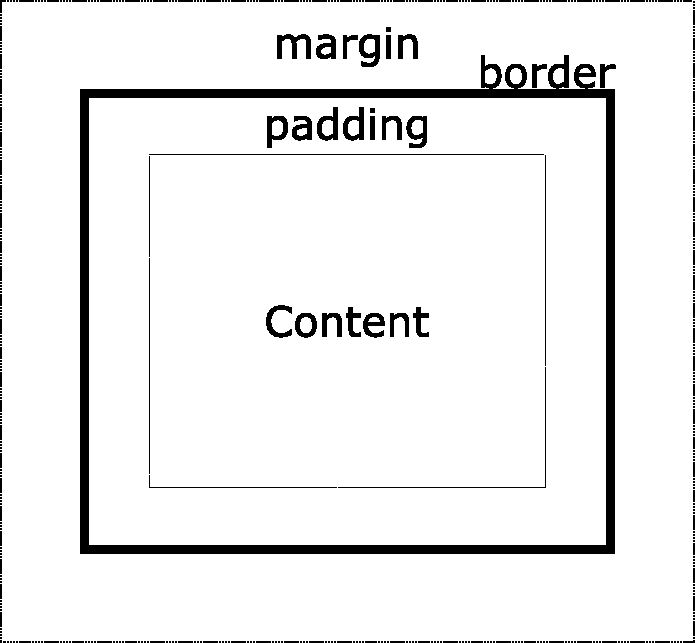
\includegraphics[keepaspectratio,width=\linewidth,height=\thirdh]
{diagrams/box-model.pdf}
\caption[CSS Box Model]{
The CSS box model defines the properties of boxes which wrap around HTML elements.
\imgcredit{Image drawn by the author of this thesis.}
}
\label{fig:BoxModel}
\end{figure}

In early versions of CSS, before the introduction of the Flexible Box
(Flexbox) layout module \parencite{CSSFlexboxFirstDraft}, the box
model was the only way to lay out elements. Style sheet authors had to
meticulously define margins of elements and their relative (or
absolute) positions in the document tree. The responsive capabilities
of this kind of layouting were very limited, because different
configurations for varying screen sizes had to be specified manually
using media queries. More complex features, like the filling of
available space, required manual implementation via scripting.





\subsection{CSS Flexbox Layout}
\label{sec:Flexbox}

CSS Flexible Box layout (Flexbox) \parencite{CSSFlexbox} is a
mechanism for one-dimensional layout of elements in either rows or
columns. This one-dimensionality is what separates it from grid-based
layout, which is inherently two-dimensional.
%
Even though the first draft of the Flexbox layout module was already
published in 2009 \parencite{CSSFlexboxFirstDraft}, implementations by
browser vendors have been a slow and bug-ridden process
\parencite{CanIUseCSSFlexbox}, which held back adoption by users for
several years after its inception. More recently though, partly
through the deprecation of Internet Explorer
\parencite{IEDeprecation}, all major browsers have mature
implementations of current Flexbox standards \parencite{CSSFlexbox},
and, in most cases, fallback styling is no longer necessary.

Flexbox layouting is enabled for child elements by setting the CSS
\cssname{display} property to \code{flex} on a container element. The
direction of the layout can then be specified using the CSS
\cssname{flex-direction} property which can be set to either
\code{row} or \code{column}.
%
The items inside a Flexbox container can have either a fixed or a
relative size. When items should be sized relative to the size of
their containers, the proportions of how the available space should be
divided can be controlled using ratios. These ratios can be set on
item elements via the CSS \cssname{flex} property.

Another important feature of Flexbox layout is the controllable
spacing of items, which can be specified separately for both the main
axis and the cross axis of the layout. Spacing along the main axis can
be configured with the CSS \cssname{justify-content} property, which
can take a number of different values and is illustrated in
Figure~\ref{fig:FlexboxJustifyContent}. Alignment of items on the
cross axis is achieved either by the CSS \cssname{align-items}
property on the container element or the CSS \cssname{align-self}
property on the items themselves.

\begin{figure}[tp]
\centering
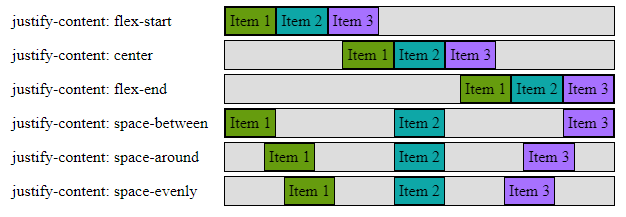
\includegraphics[keepaspectratio,width=\linewidth,height=\thirdh]
{images/flexbox-justify-content.png}
\caption[Flexbox CSS \cssname{justify-content} Property]{
The CSS \cssname{justify-content} property is used to distribute
items along the main axis of a Flexbox container. 
\imgcredit{Image created by the author of this thesis.}
}
\label{fig:FlexboxJustifyContent}
\end{figure}


This section only grazed the surface of what is possible with the
Flexbox layout module. There are many more useful CSS properties like
\cssname{flex-grow}, \cssname{flex-shrink}, and \cssname{flex-wrap}.
For a more detailed look at this topic it is recommended to review the
specification \parencite{CSSFlexbox} and read the excellent tutorial
by Chris Coyier \parencite{Coyier-FlexboxGuide}.





\subsection{CSS Grid Layout}
\label{sec:Grid}

The CSS Grid Layout Module \parencite{CSSGrid} defines the layout of
elements in a two-dimensional grid. The initial proposal of the CSS
Grid layout module was published in 2011 \parencite{CSSGridFirstDraft}
and has been further refined over the years. At the time of writing,
even though it still exists as merely a candidate recommendation for
standardization \parencite{CSSGrid}, many browsers have already
adopted it. Similar to the adoption of Flexbox, the history of browser
adoption of CSS Grid was initially strewn with inconsistencies and
bugs. However, in 2017 the major browsers Chrome, Firefox, Safari, and
Edge removed the need for vendor prefixes and implementations are now
considered stable \parencite{CanIUseCSSGrid}.

Grid layout of elements is enabled by setting the CSS
\cssname{display} property to \code{grid} on their container. The grid
in which items shall be laid out is then defined using the CSS
\cssname{grid-template-rows} and \cssname{grid-template-columns}
properties. In addition, the CSS \cssname{grid-template} property can
be used as a shorthand to simultaneously specify both the rows and
columns of a grid.
%
Item elements need to specify the cell of the grid into which they
shall be positioned. This is done with the CSS \cssname{grid-row} and
\cssname{grid-column} properties, which take the corresponding row and
column indices as values. Items can also be configured to span
multiple cells by specifying index ranges as the values of those
properties.

Every cell in a grid can also be assigned a specific name via the CSS
\cssname{grid-template-areas} property on the grid container element.
The items within the grid can then position themselves in specifically
named grid cells using the CSS \cssname{grid-area} property instead of
directly setting the row and column indices. The benefit of
positioning items this way is that the structure of the grid can be
freely changed without having to respecify the cells in which items
belong. As long as the new layout still specifies the same names of
cells somewhere in the grid, the items will be automatically placed at
their new positions.

There are also properties which control the layout of items within
grid cells and the layout of grid cells themselves. Similar to
Flexbox, this can be configured with the CSS \cssname{align-items} and
\cssname{justify-items} properties for laying out within grid cells,
and the CSS \cssname{align-content} and \cssname{justify-content}
properties for laying out the grid cells themselves. The latter
\cssname{*-content} properties only make sense when the cells do not
cover the full area of the grid. For a visual comparison between the
\cssname{*-items} and \cssname{*-content} properties, see
Figure~\ref{fig:GridLayoutProperties}.


\begin{figure}[tp]
\centering
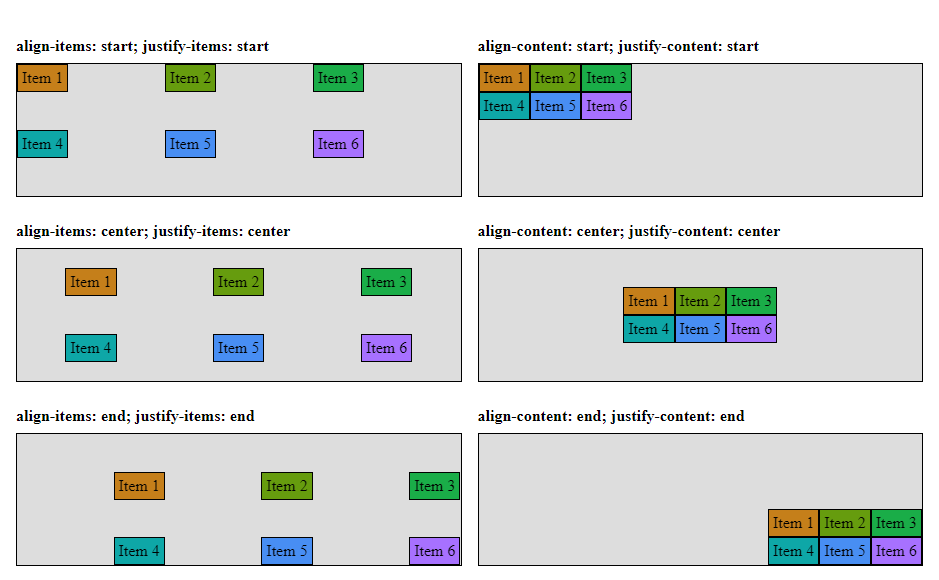
\includegraphics[keepaspectratio,width=\linewidth,height=\halfh]
{images/grid-layout-properties.png}
\caption[Grid Layout Property Comparision]{
The \cssname{*-items} properties are used to lay out items within
their grid cells, whereas the \cssname{*-content} properties are
used to lay out the grid cells themselves. 
\imgcredit{Image created by the author of this thesis.}
}
\label{fig:GridLayoutProperties}
\end{figure}


There is some apparent overlap between the CSS Grid and Flexbox layout
modules. At first sight, it seems like Grid layout supersedes Flexbox
layout, because everything which can be done using Flexbox layout can
also be done with Grid layout. While that is true, the inherent
difference in dimensionality and the resulting syntactic
characteristics lead to better suitability of one technology over the
other, depending on the context of use. As a general rule
\parencite{CSSGridVsFlexbox}, top-level layouts which require
two-dimensional positioning of elements are usually best implemented
using a Grid layout, whereas low-level layouts which merely need
laying out on a one-dimensional axis are better implemented using a
Flexbox layout.

For more details, the CSS Grid specification \parencite{CSSGrid} and
other sources like \textcite{GridLayoutInCSS} and
\textcite{House-GridGuide} are recommended.




\section{JavaScript (JS)}
\label{sec:JS}

JavaScript was originally developed as a client-side scripting
language run by an interpreter (engine) inside the web browser.
Nowadays, there are also standalone JavaScript engines and
environments like NodeJS \parencite{NodeJS}. JavaScript is a
multi-paradigm language which supports event-driven, as well as
functional and imperative programming. Driven by the popularity of the
web, JavaScript is currently the most used programming language
worldwide \parencite{StatisticProgrammingLanguageUsage}.

JavaScript was initially created by Netscape in 1995
\parencite{JSFirstRelease}. Before that, websites were only able to
display static content, which drastically limited the usefulness of
the web. Microsoft seemingly saw JavaScript as a potentially
revolutionary development, because they reverse-engineered Netscape's
implementation and published their own version of the language for
Internet Explorer in 1996 \parencite{JSIERelease}. The two
implementations were noticeably different from one another and the
uncontested monopoly of the Internet Explorer
\parencite{BrowserMarketShareEarly} held back standardization efforts
undertaken by Netscape \parencite{ECMAScript1}. When Firefox was
released in 2004 \parencite{FirefoxFirstRelease} and Chrome in 2008
\parencite{ChromeFirstRelease}, they quickly gained a considerable
share of the market \parencite{BrowserMarketShare}, as shown in
Figure~\ref{fig:BrowserMarketShare}. Galvanized by this new market
reality, all major browser vendors collaborated on the standardization
of JavaScript as ECMAScript 5 in 2009 \parencite{ECMAScript5}. Since
then, JavaScript has been continuously developed and its later
versions ECMAScript 2015 to 2021
\parencite{ECMAScript6, ECMAScript7, ECMAScript8, ECMAScript9, ECMAScript10, ECMAScript11, ECMAScript12}
are widely supported.


\begin{figure}[tp]
\centering
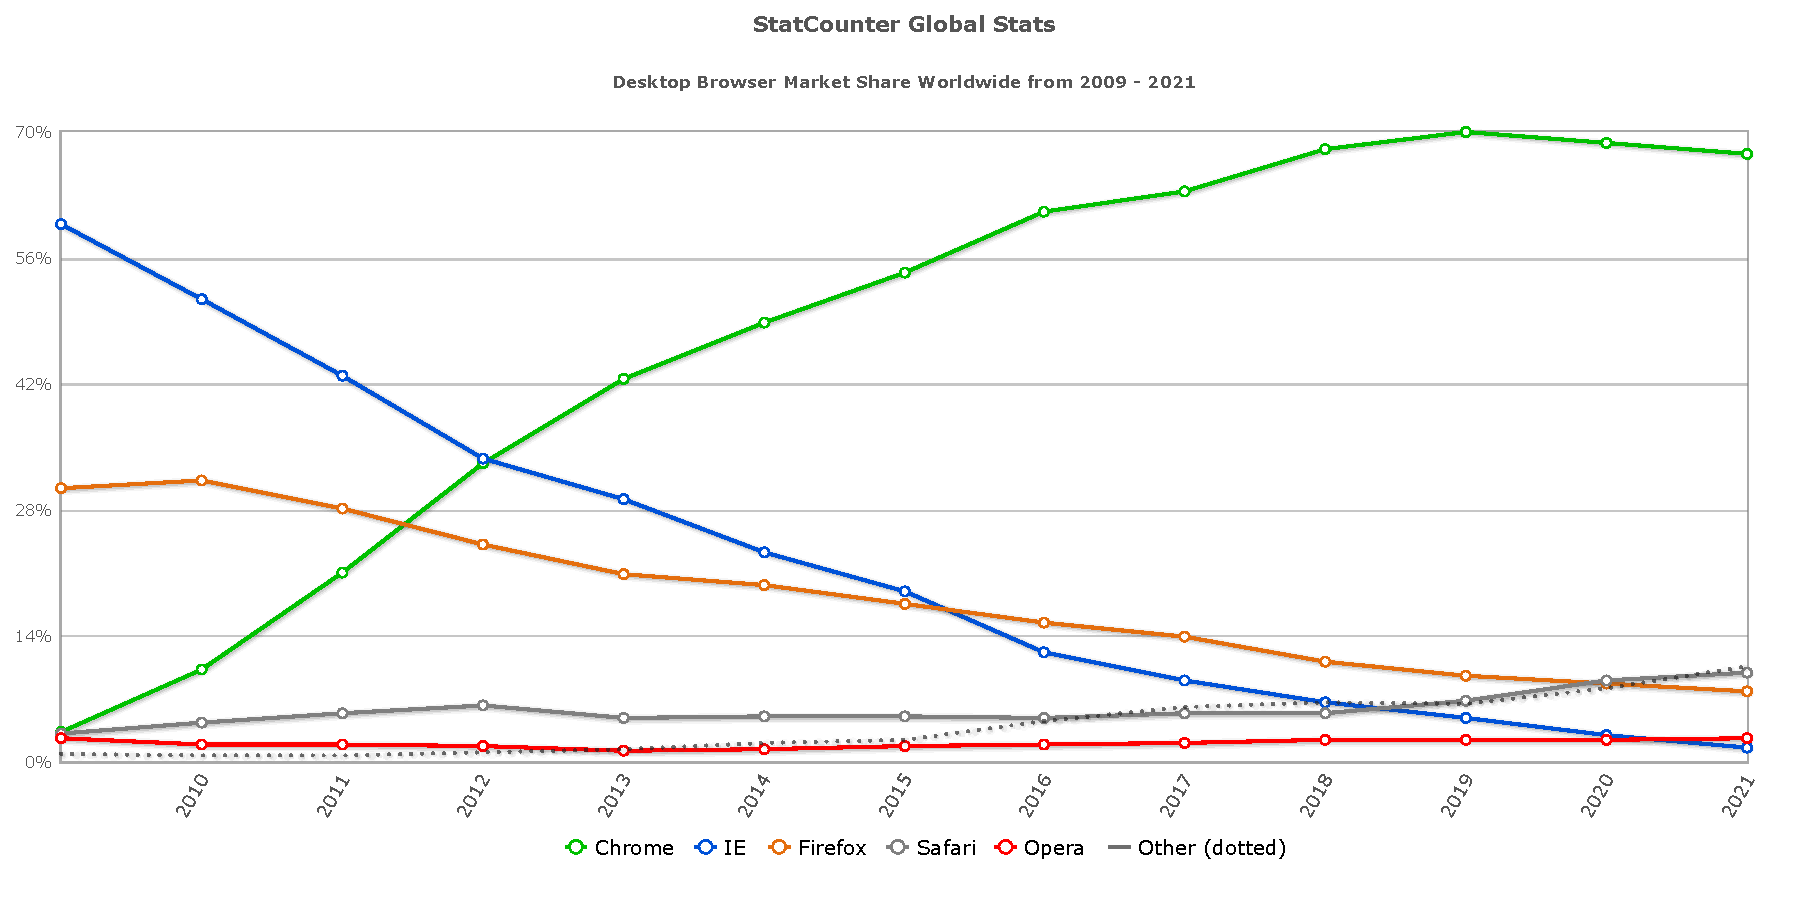
\includegraphics[keepaspectratio,width=\linewidth,height=\fullh / 3]{diagrams/browser-market-share.pdf}
\caption[Desktop Browser Market Share]{
  Since their release, Firefox and Chrome have contested the monopoly of the Internet Explorer and continuously gained more market share. 
  Recently, Chrome seems to be gaining an increasingly strong position within the market. 
  \imgcredit{Image taken from \textcite{BrowserMarketShare}}}
\label{fig:BrowserMarketShare}
\end{figure}


RespVis is a browser-based library which is designed to run within the
JavaScript engine of a browser. It builds heavily on widely supported
Web APIs, which are JavaScript modules specifically meant for
development of web pages. These Web APIs are standardized by the W3C
and each browser has to individually implement them in their
JavaScript engine.

The most popular Web API, which every web developer is familiar with,
is the Document Object Model (DOM). The DOM is the programming
interface and data representation of a web page or document.
Internally, a document is modeled as a tree of objects, where each
object corresponds to a specific HTML or SVG element in the document
hierarchy and its associated data and functions. In addition to the
querying of elements, the DOM also defines functionality to mutate
them and their attributes, as well as functionality for handling and
dispatching events. It also exposes the mechanism of
\modname{MutationObservers}, which are used to observe changes of
attributes and children in the document tree. The initial
specification of the DOM was published in 1997 \parencite{DOM1}. It
is currently maintained as a living standard by the WHATWG
\parencite{DOM}.

Another important Web API in the context of this work is the
\modname{ResizeObserver} API. It provides the ability to observe an
element's size and respond to changes, which increases the responsive
capabilities of websites. Previously, scripts could only respond to
changes in the overall viewport size via the \code{resize} event
on the \code{window} object, but this meant that changes of an
individual element's size through attribute changes could not be
detected. This limitation is fixed with the \modname{ResizeObserver}
API, which is already fully supported by all modern browsers, even
though it has so far only been published as an editor's draft
\parencite{ResizeObserver}.






\section{TypeScript (TS)}
\label{sec:TS}

TypeScript (TS) is a strongly-typed programming language which is
designed as an extension of JavaScript. Syntactically, it is a
superset of JavaScript which enables the annotation of properties,
variables, parameters, and return values with types. It requires a
transpiler (compiler) to convert the TypeScript code into valid
JavaScript code for a specific ECMAScript version.

Initially, TypeScript was released by Microsoft in 2012
\parencite{TSFirstRelease} to extend JavaScript with features which
were already present in more mature languages, and whose absence in
JavaScript caused difficulties when working on larger codebases. At
the time of TypeScript's initial development, it provided features
which would later be offered by ECMAScript 6, including a module
system to be able to split source code into reusable chunks and a
class system to aid object-oriented development. TypeScript code using
these features could then be transpiled into standard-conformant
JavaScript code, which could be interpreted by JavaScript engines of
the time. At the time of writing, ECMAScript 6 is widely supported by
all modern browsers and therefore the main benefit of TypeScript over
JavaScript lies in its provision of a static type system.

The extension of JavaScript with a static type system brings many
benefits, including the improved tooling which comes with
type-annotated code. Tools such as linters \parencite{ESLint} are able
to point out errors early in development and assist developers with
automated fixes, improved code completion, and code navigation.
Additionally, studies like \textcite{ToTypeOrNotToType} looked at
software bugs in publicly available codebases and found that 15\% of
them could have been prevented with static type checking.

The TypeScript type system was designed to support JavaScript
constructs as completely as possible, via structural types and unified
object types. Another goal was to make the type annotation of
JavaScript code as effortless as possible to improve adoption by
existing projects. This was done by consciously allowing the type
system to be statically unsound via gradual typing and also by
employing type inference to reduce the number of necessary
annotations. The major properties of TypeScript's type system design
are summarized in Table~\ref{tab:TSTypeSystemDesignProperties}.


\begin{table}[tp]
\tablestretch
\rowcolors{2}{}{tablerowcolour}
\centering
\begin{tabularx}{\linewidth}{>{\kern-\tabcolsep}lX<{\kern-\tabcolsep}}
\toprule
Design Property & Description \\
\midrule
Full erasure         &
Types are completely removed by the compiler, there is no type checking at runtime. \\
%
Type inference       &
Many types can be inferred from usage, minimizing the number of types which have to be explicitly stated. \\
%
Gradual typing       &
Type checking can be selectively prevented using the dynamic type \lstinline{any}. \\
%
Structural types     &
Types are defined via their structure as opposed to via their names.
This better fits JavaScript, where objects are usually custom-built and used based on their shapes. \\
%
Unified object types &
A type can simultaneously describe objects, functions, and arrays.
These constructs are common in JavaScript and thus TypeScript needs to support their typing. \\
\bottomrule
\end{tabularx}
\caption[TypeScript Type System Design Properties]{
A summary of the major design properties on which TypeScript's type system is built.
\imgcredit{Table created by the author of this thesis with data from \textcite{UnderstandingTS}.}
}
\label{tab:TSTypeSystemDesignProperties}
\end{table}









\section{Web Graphics}
\label{sec:WebGraphics}

Graphics are used as a medium for visual expression to enhance the
representation of information on the web. There are many fields of
application like the integration of maps, photographs, or charts in a
web page. Multiple complementary technologies exist for web graphics,
each with particular strengths and weaknesses depending on the use
case. These technologies include pixel-based raster images, Scalable
Vector Graphics (SVG), and 2d and 3d graphics through the
\elname{<canvas>} element.



\subsection{Raster Images}
\label{sec:RasterImages}

A raster image represents a graphic as a rectangular, two-dimensional
grid of pixels with a fixed size (resolution) in each dimension.
Whenever a raster image is scaled up or down to a different size,
visual artifacts become very apparent, as can be seen in
Figure~\ref{fig:RasterImage}. Raster images are either created by
image capturing devices or special editing software and saved as
binary files in varying formats. The most widely used formats for
raster images are JPEG \parencite{JPEG} and PNG (Portable Network
Graphics) \parencite{PNG}. JPEG has lossy compression, which achieves
low file sizes whilst retaining reasonable image quality, and is
typically used for photographs. PNG has lossless compression, which
compresses well whilst preserving every original pixel as is, and also
supports transparency. Both formats support progressive rendering as
an image is loaded.


\begin{figure}[tp]
\centering
\subfloat[Intended size.]{%
\hspace{1cm}

\includegraphics[scale=1]{images/circle.png}
\hspace{1cm}
\label{fig:RasterImage1}
}
\hspace{1cm}
\subfloat[Two and a half times intended size.]{%
\hspace{1cm}

\includegraphics[scale=2.5]{images/circle.png}
\hspace{1cm}
\label{fig:RasterImage2}
}
\caption[Raster Image Scaling]{%
A raster image of a circle.
Pixelation artifacts become very apparent when a raster image
is scaled to a different size.
\imgcredit{Image created by the author of this thesis.}
}
\label{fig:RasterImage}
\end{figure}


Raster images are embedded into documents in binary format. This means
that the contents of the graphic are not accessible in a non-visual
representation. To make the information accessible to visually
impaired people, an additional textual description of the graphic's
content must be provided via the \attrname{alt} and
\attrname{longdesc} attributes.





\subsection{Scalable Vector Graphics (SVG)}
\label{sec:SVG}

Vector graphics describe an image in terms of objects and shapes, such
as lines, circles, polygons, and text. They can be scaled freely
without loss of quality. Scalable Vector Graphics (SVG) is an
XML-based format for vector graphics. It was initially published by
the W3C in 1999 \parencite{SVG1}, SVG 1.1 \parencite{SVG11} is the
latest version that is widely supported by browsers, and support for
SVG 2 \parencite{SVG2} is currently on its way. Graphics in an SVG
file can be specified in a normalised coordinate space (inside a
viewBox), enabling them to be freely scaled. Since SVG files are XML,
they can be created with any text editor, but numerous tools and
editors such as Inkscape \parencite{Inkscape} and Illustrator
\parencite{Illustrator} exist to create or export SVG. A simple example
of an SVG document containing a single circle can be seen in
Listing~\ref{list:SVG}, with its visualization shown in
Figure~\ref{fig:SVG}.

\begin{samepage}
\lstinputlisting[%
  float=tp,
  aboveskip=\floatsep,
  belowskip=\floatsep,
  xleftmargin=0cm,              % no extra margins for floats
  xrightmargin=0cm,             % no extra margins for floats
  basicstyle=\footnotesize\ttfamily,
  frame=shadowbox,
  numbers=left,
  label=list:SVG,
  caption={%
[SVG Document Containing a Circle]%
A simple SVG document containing a \elname{<circle>} element.
The visual representation of this document in different sizes
is shown in Figure~\ref{fig:SVG}.
}
]{listings/circle.svg}
\end{samepage}


\begin{figure}[tp]
\centering
\subfloat[Intended size.]{%
\hspace{1cm}

\includegraphics[scale=1]{images/circle.pdf}
\hspace{1cm}
\label{fig:SVG1}
}
\hspace{1cm}
\subfloat[Two and a half times intended size.]{%
\hspace{1cm}

\includegraphics[scale=2.5]{images/circle.pdf}
\hspace{1cm}
\label{fig:SVG2}
}
\caption[SVG Scaling]{%
SVG documents can be scaled freely without pixelation artifacts.
Here, the SVG document from Listing~\ref{list:SVG} is shown.
\imgcredit{Image created by the author of this thesis.}
}
\label{fig:SVG}
\end{figure}



The encoding in XML leads to SVG being the best format to represent
graphics in terms of accessibility. Graphics are directly saved in a
hierarchical and textual form which describes their shapes and how
they are composed. In addition to the shapes being inherently
accessible, the various elements of an SVG document can be annotated
with further information to aid comprehension when consumed in a
non-visual way.

SVG files are XML documents whose meta format is described in a
special SVG namespace. Web browsers support mixing of HTML and SVG
elements in a web page, and the SVG elements can be accessed by
scripts via the DOM Web API just like HTML elements.

The most widely supported way of styling SVG elements is via
attributes, which is supported by every software dealing with SVG
files. However, the specification aims for maximum compatibility with
HTML, and therefore it is also possible to use CSS to style and
animate SVG elements when they are rendered in a browser. Using CSS to
separate presentation from content has many benefits, which were
already described in Section~\ref{sec:CSS}. Unfortunately, it is not
possible to style every SVG attribute with CSS, only so-called
presentation attributes like \attrname{fill} and \attrname{stroke-width}
are available through CSS. These presentation attributes are listed in
the SVG specification \parencite{SVG11} and will be extended by
additional attributes like \cssname{x}, \cssname{y}, \cssname{width}
and \cssname{height} in upcoming releases \parencite{SVG2}.


\subsection{Canvas (2D)}
\label{sec:Canvas2D}

The \elname{<canvas>} element was introduced in HTML5
\parencite{HTML5} and is used to define a two-dimensional, rectangular
region in a document which can be drawn into by scripts. Even though
rendering of dynamic graphics as \elname{<canvas>} elements is often
faster than representing them as SVG documents, their use is
explicitly discouraged by the WHATWG \parencite{HTML} when another
suitable representation is possible. The reasons for this are that
\elname{<canvas>} elements are not compatible with other web
technologies like CSS or the DOM Web API and because the resulting
rendering provides only very limited possibilities for accessibility.

The graphics are drawn via a low-level API provided by the rendering
context of a particular canvas. The two most significant rendering
contexts are \code{2d} and \code{webgl}.

The \code{2d} rendering context enables platform-independent 2d
rendering via a software renderer, whose API is standardized directly
in the canvas specification \parencite{Canvas2D}. An example of an
HTML document containing two differently sized canvases into which
responsive circles are drawn using a 2d rendering context can be seen
in Listing~\ref{list:Canvas} with the corresponding visual output in
Figure~\ref{fig:Canvas}.


\begin{samepage}
\lstinputlisting[%
  float=tp,
  aboveskip=\floatsep,
  belowskip=\floatsep,
  xleftmargin=0cm,              % no extra margins for floats
  xrightmargin=0cm,             % no extra margins for floats
  basicstyle=\footnotesize\ttfamily,
  frame=shadowbox,
  numbers=left,
  label=list:Canvas,
  caption={%
[Canvas With Responsive Circles]%
A basic HTML document containing two canvases of different sizes
which render circles relative to the canvas size. 
The visual representation of this document is shown in Figure~\ref{fig:Canvas}.
}
]{listings/canvas.html}
\end{samepage}


\begin{figure}[tp]
\centering
\subfloat[100-pixel canvas.]{%
\hspace{1cm}

\includegraphics[scale=0.5]{images/canvas100.png}
\hspace{1cm}
\label{fig:Canvas1}
}
\hspace{1cm}
\subfloat[250-pixel canvas.]{%

\includegraphics[scale=0.5]{images/canvas250.png}
\label{fig:Canvas2}
}
\caption[Canvas With Responsive Circles]{
Responsive rendering of graphics inside \elname{<canvas>} elements has to be
implemented manually by calculating everything relative to its dimensions. 
This figure shows the visual output
of the canvas example in Listing~\ref{list:Canvas}. 
\imgcredit{Image created by the author of this thesis.}
}
\label{fig:Canvas}
\end{figure}







\subsection{Canvas (WebGL)}
\label{sec:CanvasWebGL}

The \code{webgl} rendering context enables 3d drawing through the
WebGL version 1 API \parencite{WebGL1}. The \code{webgl2}
rendering context enables 3d drawing through the WebGL version 2 API
\parencite{WebGL2}. WebGL-based rendering is hardware-accelerated and
often much faster than rendering via a 2d canvas or SVG. It is also
possible to render 2d graphics using a WebGL render context, but the
necessary setup and rendering API is rather complex.   



\section{Layout Engines}
\label{sec:LayoutEngines}

A layout engine is used to calculate the boundary coordinates of
visual components based on input components annotated with layout
constraints. These layout constraints describe the size and position
of components and their relationships between each other in a syntax
understood by the layout engine. For browser-based layout engines, the
input components are normally declared as HTML documents, which are
constrained using CSS. More low-level layout engines require custom
formats, which usually involve a hierarchy of objects constrained
using specific properties. The most relevant layout engines in the
context of this work are summarized in the following sections.


\subsection{Browser Engines}
\label{sec:BrowserEngines}

The purpose of a browser engine is to transform document and any
additional resources, like CSS, into a visual representation. A
browser engine is a core component of every web browser, and it is
responsible for laying out elements and rendering them.  The
terminology of browser engines is ill-defined, with them sometimes
also being referred to as layout or render engines. Theoretically, the
layout and render processes could be separated into different
components, but in practice they are tightly-coupled into a combined
component, which will be referred to as a browser engine in this work.
Some notable browser engines are WebKit \parencite{WebKit}, Blink
\parencite{Blink}, and Gecko \parencite{Gecko}.

In a browser engine, the layout of elements is constrained with CSS,
which yields great flexibility as already described in
Section~\ref{sec:CSS}. A range of mechanisms is available to precisely
control the layout of elements, like the Flexible Box and Grid layout
modules, which can also be used in combination.

The layout module of a browser engine can only be invoked directly by
browsers to position HTML elements in actively rendered documents. To
use it for calculating layouts of non-HTML constructs, they must be
replicated in active documents, so they can be parsed, laid out and
rendered by the browser engine. These replicated constructs do not
necessarily have to be visible, and they could also be removed from
the document after the layout has been acquired, meaning they do not
need to be noticeable at all. A strong limitation of using browser
engines to calculate layouts is that it requires a browser runtime to
work and, even though there are solutions like Electron
\parencite{Electron} available, which enable development of desktop
applications using web technologies, this limitation forces
applications into a very specific stack of technologies.



\subsection{Yoga}
\label{sec:Yoga}

Yoga \parencite{Yoga} is a layout engine which enables the computation
of layouts constrained using the grammar defined in the CSS Flexible
Box layout module (see Section~\ref{sec:Flexbox}). It has been
maintained by Facebook as an open-source project since 2016
\parencite{YogaRelease}, with the goal of providing a small and
high-performance library which can be used across all platforms. Yoga
is implemented in C/C++, which works on a myriad of devices, with
bindings available for other platforms like JavaScript, Android, and
iOS. It has been widely adopted and is used to perform layouting in
major frameworks such as React Native \parencite{ReactNative}, Litho
\parencite{Litho}, and ComponentKit \parencite{ComponentKit}.



\subsection{FaberJS}
\label{sec:FaberJS}

FaberJS \parencite{FaberJS} is a layout engine very similar to the
Yoga layout engine in that it enables the computation of layouts for
constructs other than HTML documents, using a layout grammar
originally created for CSS. In contrast to Yoga, which is used to
create one-dimensional layouts using the Flexbox layout grammar,
FaberJS implements a two-dimensional layout algorithm built on the
grammar of the CSS Grid layout module (see Section~\ref{sec:Grid}).
This inherently two-dimensional approach to layouting is more suited
to information visualization than a one-dimensional approach. FaberJS
is an open-source JavaScript project developed since 2019 by
Idera. Even though the layouts it computes are constrained with the
Grid Layout grammar, it only supports a subset the functionality
defined in the original CSS module. Some examples of missing
functionaly include missing support for margins, gaps, and the
\cssname{*-content} and \cssname{grid-auto-*} properties. Working
around the limitations caused by these missing features is
non-trivial, and it seems unlikely that support for them will be added
by the FaberJS maintainers in the near future because, at the time of
writing, the project has not been updated in nearly two years.






\section{Responsive Web Design}
\label{sec:RWD}

Influenced by the increasing use of mobile devices and their vastly
varying screen sizes, responsive web design has established itself as
the predominant way of designing web pages. The core idea of
responsive web design is that instead of designing pages for different
types of devices, website authors create a single design for a page,
which adapts to the characteristics of the consuming device. The term
\enquote{Responsive Web Design} was initially defined by
\textcite{Marcotte-ALA-RWD} and later compiled into a book
\parencite{ResponsiveWebDesign}, in which the author differentiates
between flexible and responsive web designs. A flexible web design,
which merely fluidly scales blocks of content to make them fit into
the width of a browser window, is not enough to provide a good
experience for users. Such designs will work well enough for similarly
sized viewports to the one they were created for, but they will lead
to noticeable artifacts on lower resolutions.

These problems can be avoided by positioning the individual components
of a page in a manner which provides them with enough space to render
correctly. This can be achieved by using CSS media queries to adapt
the overall layout of a page to the dimensions of the consuming
device. Another crucial part of responsive web design is to support
the different modes of interaction inherent to the various types of
devices used to access the web. Desktop users might access a website
using a mouse, mobile device users typically interact via a
touchscreen, and yet others might consume a page in a purely textual
form with a screen reader and interact via a keyboard. It is one of
the mantras of responsive web design to provide smooth and complete
access to information to all users, regardless of the device they are
using.
         

\cleardoublepage

\chapter{Information Visualization}
\label{chap:InfoVis}

Information visualization seeks to use interactive graphics to assist
in the analysis and presentation of abstract information. Information
visualization builds on capabilities of human visual perception,
including the rapid scanning, recognition, and recall of visual
information, as well as the automatic detection of visual patterns. In
contrast to textual representations of data, the processing of
well-designed visualizations requires less cognitive effort,
because it leverages features of the human visual processing
system. One of these features is \emph{preattentive processing},
whereby certain visual attributes can be processed very quickly and
without conscious effort \parencite{PreattentiveProcessing}.
% KA give an example of a pre-attentive feature


In addition to visuals being easier to assimilate by humans, a purely
textual and statistical view of data can also lead to erroneous
assumptions. This is demonstrated in Anscombe's famous example of four
completely different datasets (variables in $x$ and $y$) having
identical summary statistics (mean and standard deviation), called
Anscombe's Quartet \parencite{AnscombesQuartet}, shown in
Table~\ref{tab:AnscombeTable}. An observer trying to understand these
datasets from their summary statistics alone might mistakenly deem
them to be identical. Their inequality only becomes obvious after
carefully examining and comparing the individual entries in the
datasets themselves.
%
However, the differences in the four datasets are immediately obvious
when plotted graphically, as can be seen in
Figure~\ref{fig:AnscombePlot}. Even though Anscombe's Quartet is
likely the most famous example demonstrating this characteristic, it
is certainly not the only example, as has been shown by
\textcite{GenDataIdenticalStatisticsDissimilarGraphics}.



\begin{table}[tp]
\centering
\tablestretch
\rowcolors{3}{tablerowcolour}{}
\begin{small}
\begin{tabular}{>{\kern-\tabcolsep}rcrrcrrcrrcrr<{\kern-\tabcolsep}}
\toprule
\hiderowcolors
  & \phantom{i} &
  \multicolumn{2}{c}{$\mathbf{v_1}$} & \phantom{a} &
  \multicolumn{2}{c}{$\mathbf{v_2}$} & \phantom{a} &
  \multicolumn{2}{c}{$\mathbf{v_3}$} & \phantom{a} &
  \multicolumn{2}{c}{$\mathbf{v_4}$} \\
\cmidrule(l{1em}r){3-4}\cmidrule(l{1em}r){6-7}\cmidrule(l{1em}r){9-10}\cmidrule(l{1em}r){12-13}
  & & $x_1$ &  $y_1$ & &  $x_2$ & $y_2$ & & $x_3$ &  $y_3$ & &  $x_4$ &  $y_4$ \\
\midrule
\showrowcolors
  & & 10.00 &   8.04 & &  10.00 &  9.14 & &  10.00 &   7.46 & &   8.00 &   6.58 \\
  & &  8.00 &   6.95 & &   8.00 &  8.14 & &   8.00 &   6.77 & &   8.00 &   5.76 \\
  & & 13.00 &   7.58 & &  13.00 &  8.74 & &  13.00 &  12.74 & &   8.00 &   7.71 \\
  & &  9.00 &   8.81 & &   9.00 &  8.77 & &   9.00 &   7.11 & &   8.00 &   8.84 \\
  & & 11.00 &   8.33 & &  11.00 &  9.26 & &  11.00 &   7.81 & &   8.00 &   8.47 \\
  & & 14.00 &   9.96 & &  14.00 &  8.10 & &  14.00 &   8.84 & &   8.00 &   7.04 \\
  & &  6.00 &   7.24 & &   6.00 &  6.13 & &   6.00 &   6.08 & &   8.00 &   5.25 \\
  & &  4.00 &   4.26 & &   4.00 &  3.10 & &   4.00 &   5.39 & &  19.00 &  12.50 \\
  & & 12.00 &  10.84 & &  12.00 &  9.13 & &  12.00 &   8.15 & &   8.00 &   5.56 \\
  & &  7.00 &   4.82 & &   7.00 &  7.26 & &   7.00 &   6.42 & &   8.00 &   7.91 \\
  & &  5.00 &   5.68 & &   5.00 &  4.74 & &   5.00 &   5.73 & &   8.00 &   6.89 \\
\hiderowcolors
\addlinespace[0.5em]
\textbf{mean} & &
  \textbf{9.00} & \textbf{7.50} & &
  \textbf{9.00} & \textbf{7.50} & &
  \textbf{9.00} & \textbf{7.50} & &
  \textbf{9.00} & \textbf{7.50} \\
\textbf{sd} & &
  \textbf{3.3166} & \textbf{2.0316} & &
  \textbf{3.3166} & \textbf{2.0317} & &
  \textbf{3.3166} & \textbf{2.0304} & &
  \textbf{3.3166} & \textbf{2.0306} \\
\bottomrule
\end{tabular}
\end{small}

\caption[Anscombe's Quartet in Tabular Form]
{
The four datasets (variables) in Anscombe's Quartet look identical if
only standard summary statistics like mean and standard deviation are
considered. The difference between the datasets is only apparent after
careful examination of the numbers.
}
\label{tab:AnscombeTable}
\end{table}



\begin{figure}[tp]
\centering
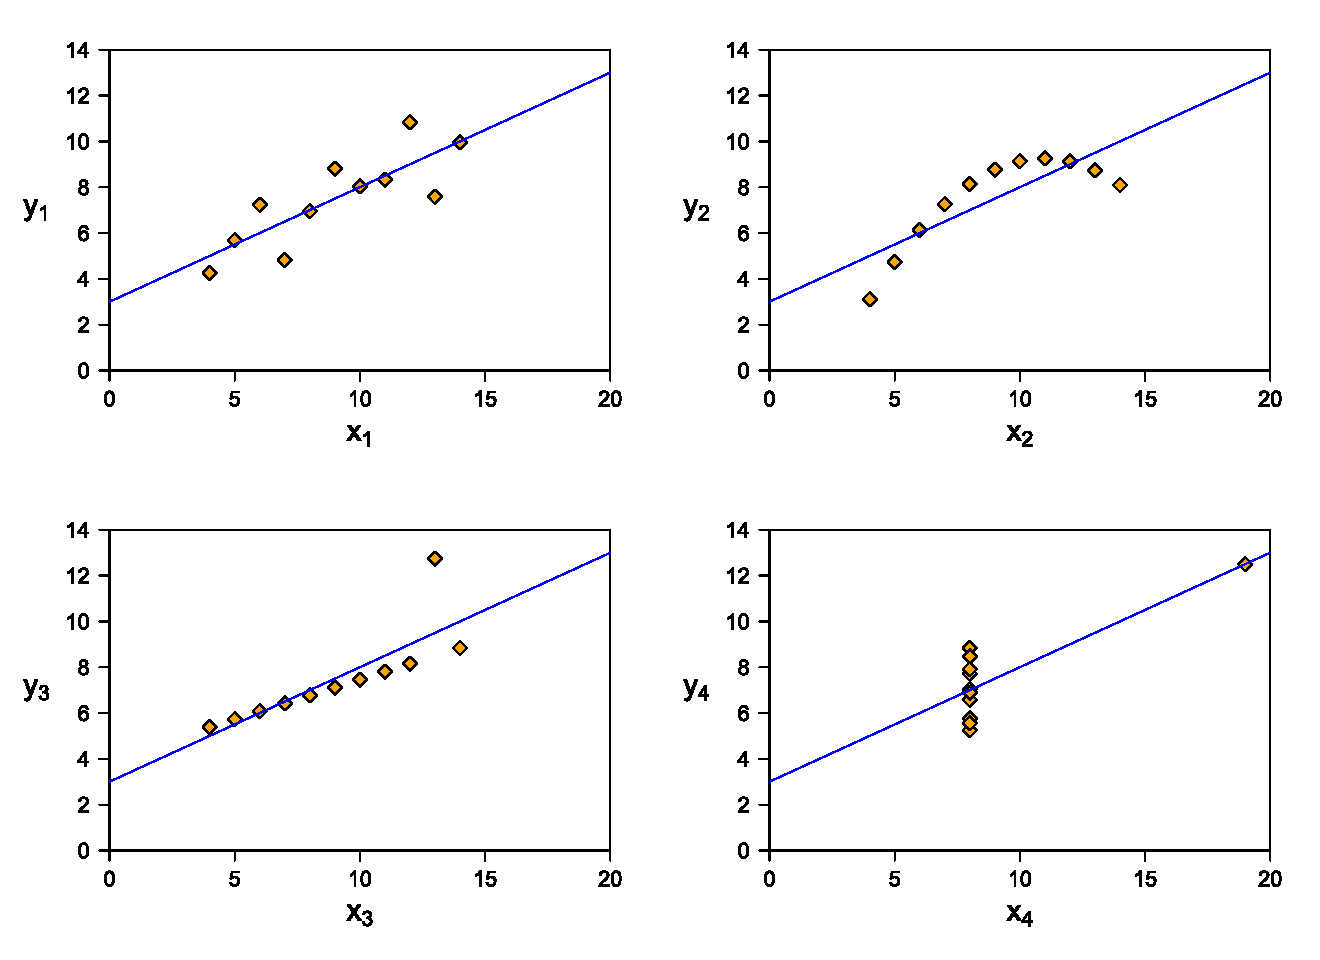
\includegraphics[keepaspectratio,width=\linewidth,height=\halfh]
{diagrams/anscombe.pdf}
\caption[Anscombe's Quartet]{
When plotted graphically, it is immediately apparent that
the four datasets in Anscombe's Quartet are very different.
\imgcredit{Image extracted from \textcite{IVISCourseNotes}.
Used with kind permission by Keith Andrews.}
}
\label{fig:AnscombePlot}
\end{figure}







This thesis adheres to the characterization of the field of
visualization as having three main subfields, as defined by
\textcite{IVISCourseNotes}:
\begin{enumerate}
\item \liintro{Information Visualization (InfoVis)}: Deals with
  abstract data, which has no inherent geometry or visual form and for
  which a suitable type of visualization has to be chosen.

\item \liintro{Geographic Visualization (GeoVis)}: Deals with
  map-based data which has inherent 2d or 3d spatial geometry.

\item \liintro{Scientific Visualization (SciVis)}: Deals with
  real-world objects having inherent 2d or 3d geometry, which
  is used as the basis for visualization.
\end{enumerate}
The often-used term \enquote{data visualization} (\emph{DataVis}) is
defined as the combination (union) of information visualization and
geographic visualization.


Visualizations presented in an interactive medium do not merely
consist of visual representations. It is equally important to provide
means for interacting with these representations to analyze more
complex datasets. Without interactions, a visualization is just a
static image and has only very limited use when dealing with large and
multidimensional datasets. Even though the majority of attention in
the field of information visualization has been directed towards the
presentational aspect of visualizations, research has also been done
on their interactive aspects. Numerous taxonomies have been formulated
with the goal of defining the design space of interactions to support
analytic reasoning, but they vary greatly depending on the concepts
they are focusing on. Some taxonomies have been defined on the concept
of low-level interaction techniques
\parencite{TheEyesHaveIt,GrammarOfGraphics}, providing a very
system-centric view on interaction. Other taxonomies focus on user
tasks \parencite{LowLevelComponentsOfAnalyticActivity}, which are not
necessarily strongly related to interacting with visualizations.
\textcite{RoleOfInteractionInInformationVisualization} aims to provide
a view in between the purely system-centric and purely user-centric
extremes by defining a taxonomy based on what a user wants to achieve,
also known as \emph{user intent}. The categories of this taxonomy are
shown in Table~\ref{tab:UserIntentCategories}. They provide a good
framework for the discussion of interactivity in the context of
information visualization.


\begin{table}[tp]
\tablestretch
\rowcolors{2}{}{tablerowcolour}
\centering
\begin{small}
\begin{tabularx}{\linewidth}{>{\kern-\tabcolsep}lL{0.35\linewidth}X<{\kern-\tabcolsep}}
\toprule
Category & Description & Examples \\
\midrule
Select &
  Mark something as interesting. &
  Highlighted selections, placemarks, assigning classes. \\
Explore &
  Show me something else. &
  Different subset of data, panning, direct-walk. \\
Reconfigure &
  Show me a different arrangement. &
  Sorting, rearranging columns, plotting different dimensions, using an alternative projection. \\
Encode &
  Show me a different representation. &
  Changing visual encoding (color, size, shape), or even chart type. \\
Abstract / Elaborate &
  Show me more or less detail. &
  Details-on-demand, drill-down and roll-up, tooltips, zooming in and out. \\
Filter &
  Show me something conditionally. &
  Dynamic queries, range sliders, toggle buttons, query by example. \\
Connect &
  Show me related items. &
  Brushing across views, highlighting connected items on mouseover. \\
\bottomrule
\end{tabularx}
\end{small}
\caption[Categories of Interaction Based on User Intent]{
Categories of interaction with visualizations based on what
a user wants to achieve (user intent).
\imgcredit{From \textcite{RoleOfInteractionInInformationVisualization}}
}
\label{tab:UserIntentCategories}
\end{table}






\section{History of Information Visualization}

The history of information visualization goes back a long time. One of
its earliest examples dates back to the \nth{10} Century, when an
unknown astronomer created the chart about the movement of prominent
planets \parencite{CommentariiInSomniumScipionis} shown in
Figure~\ref{fig:PlanetaryMovements}.
% KA: 1175 is the 12th Century not the 10th
Other noteworthy early visualizations include the first occurrence of
the principle which \textcite{VisualDisplayOfQuantitativeInformation}
later called \enquote{small multiples} in the 1626 chart by
\textcite{RosaUrsina} demonstrating sunspot changes shown in
Figure~\ref{fig:SunspotChanges}, and the 1644 chart displaying
longitudinal distance determinations between Toledo and Rome by
Michael Florent van Langren shown in
Figure~\ref{fig:RomeToledoLongitude}.


\begin{figure}[tp]
\centering
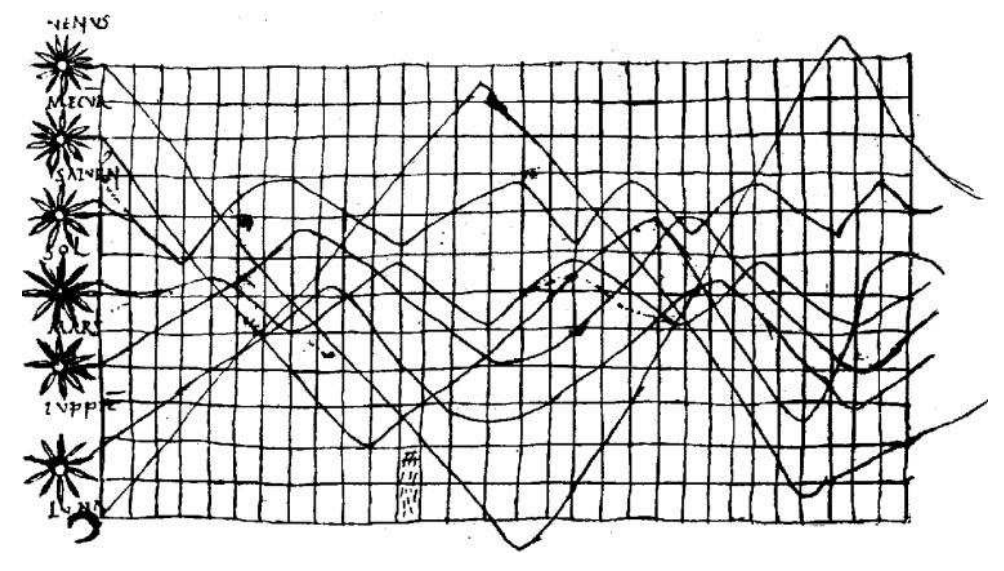
\includegraphics[keepaspectratio,width=\linewidth,height=\thirdh]
{images/planetary-movements.png}
\caption[Chart of Planetary Movements from the \nth{10} Century]{%
A line chart created by an unknown astronomer in the \nth{10} Century,
depicting the movements of seven prominent planets.
\imgcredit{Image extracted from \textcite{BriefHistoryOfDataVis}.
Original appearance in \textcite{CommentariiInSomniumScipionis}.}
}
\label{fig:PlanetaryMovements}
\end{figure}
% KA Original appearance in Macrobius [1175] ??
% Funkhouser 1936 says 10th or 11th Century



\begin{figure}[tp]
\centering
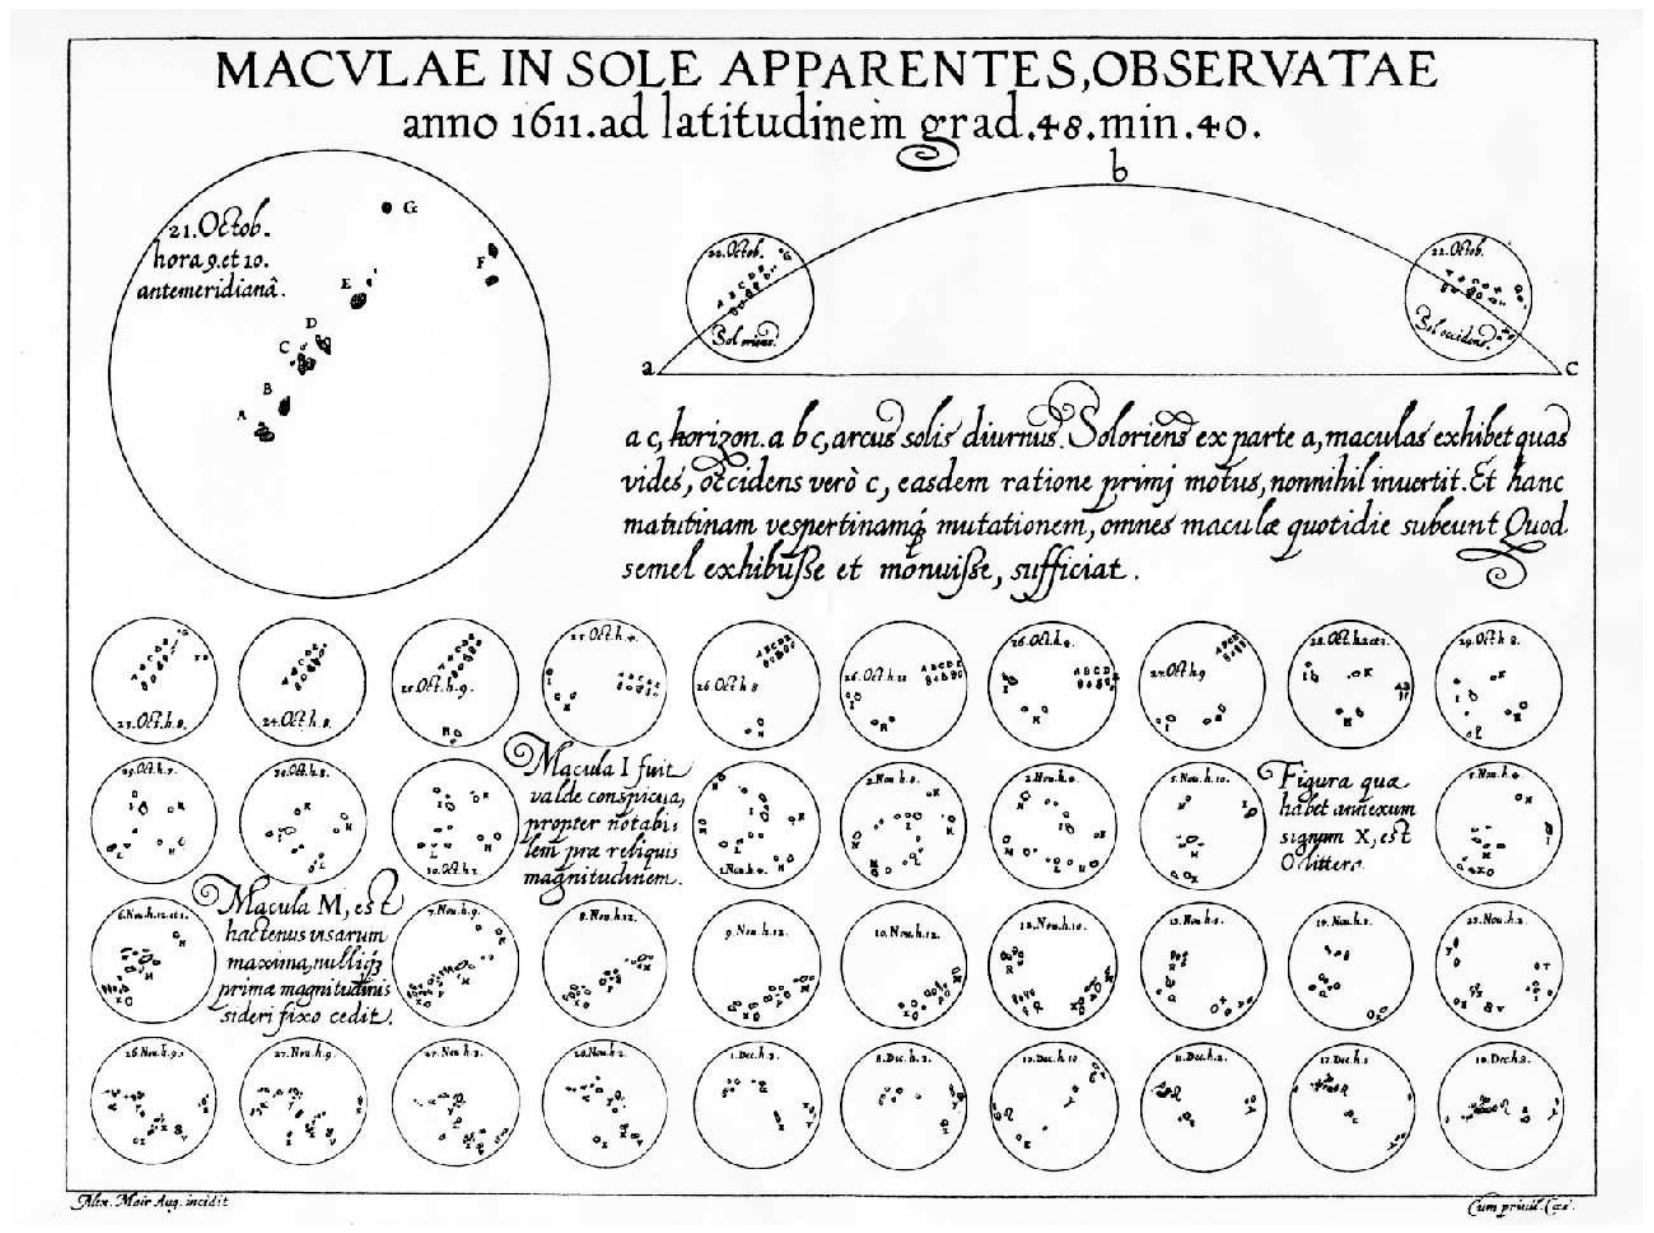
\includegraphics[keepaspectratio,width=\linewidth,height=\thirdh]
{images/sunspot-changes.png}
\caption[Chart of Changes in Sunspots from 1626]{%
The observed changes in sunspots based on recordings
of two months of data from 1611. It is the first occurrence of the
principle later called \enquote{small multiples} by
\textcite{VisualDisplayOfQuantitativeInformation}.
\imgcredit{Image extracted from \textcite{BriefHistoryOfDataVis}.
Original appearance in \textcite{RosaUrsina}.}
}
\label{fig:SunspotChanges}
\end{figure}

% https://cudl.lib.cam.ac.uk/view/PR-QQ-AST-00002-00158-B-00003/1

% Tufte, Edward R. and Peter R. Graves-Morris [1983].
% The Visual Display of Quantitative Information.
% Graphics Press, 1983. ISBN 1930824130 (cited on pages 19–20).
% KA: who is Graves-Morris ?



\begin{figure}[tp]
\centering
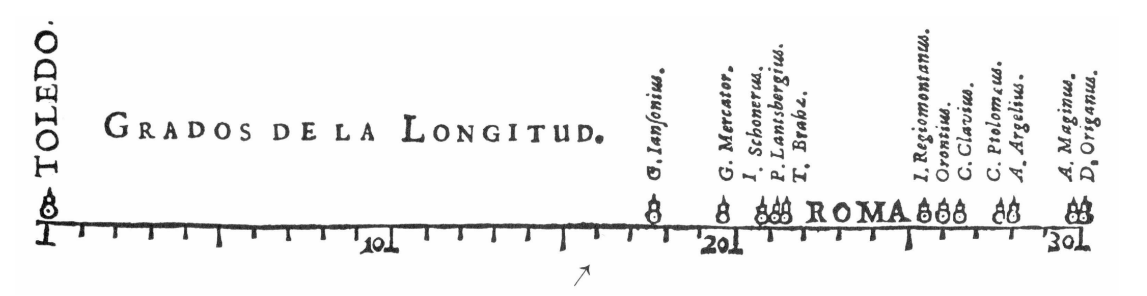
\includegraphics[keepaspectratio,width=\linewidth,height=\thirdh]
{images/rome-toledo-longitude.png}
\caption[Chart of Longitudinal Distance Determinations Between Toledo and Rome From 1644]{%
A comparison of the twelve known estimates in longitudinal
distance between Rome and Toledo by various astronomers. The correct
distance is marked by the arrow beneath. It is considered to be the
first visual representation of statistical data.
\imgcredit{Image extracted from \textcite{BriefHistoryOfDataVis}.
Original appearance in \textcite{VisualExplanations}.}
}
\label{fig:RomeToledoLongitude}
\end{figure}

% KA  how can it be the "first visual representation of statistical data"  ?

% Tufte, Visual Explanations, 1997, page 15





William Playfair (1759--1823) is considered by many to be one of the
forefathers of modern information visualization. His published works
contain the first occurrences of many graphical forms still widely
used today. In one of his earlier works
\parencite{CommercialAndPoliticalAtlas}, he introduced the concepts of
line charts (Figure~\ref{fig:PlayfairLineChart}), bar charts
(Figure~\ref{fig:PlayfairBarChart}), and area charts
(Figure~\ref{fig:PlayfairAreaChart}) to communicate economic factors
of England during the eighteenth century. In a related later work
\parencite{StatisticalBreviary}, he used the first ever published pie
and circle charts to show and compare the resources of states and
kingdoms in Europe. The charts he created are very similar to modern
ones, containing familiar concepts such as labeled axes, grids,
titles, and color-coding.



\begin{figure}[tp]
\centering
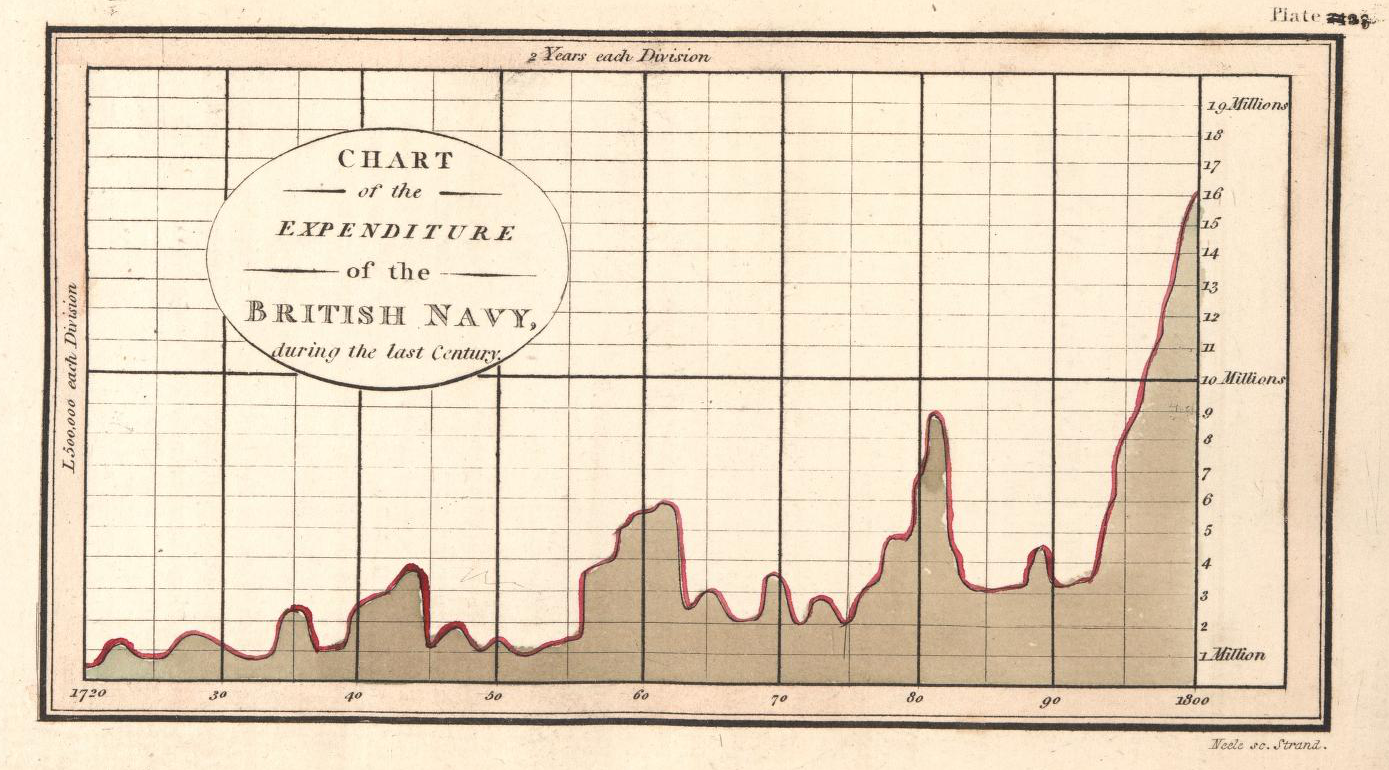
\includegraphics[keepaspectratio,width=\linewidth,height=\thirdh]
{images/playfair-line-chart.png}
\caption[Line Chart by William Playfair from 1786]{%
Line chart of the expenditure of the British Navy during the \nth{18}
Century. It was published in 1786 and is considered to be one of the
first occurrences of a line chart containing components found in
modern visualizations.
\imgcredit{Image extracted from Schoenberg Center for
Electronic Text and Image (SCETI).
Used under the terms of Creative Commons CC BY 2.5.}
}
\label{fig:PlayfairLineChart}
\end{figure}



\begin{figure}[tp]
\centering
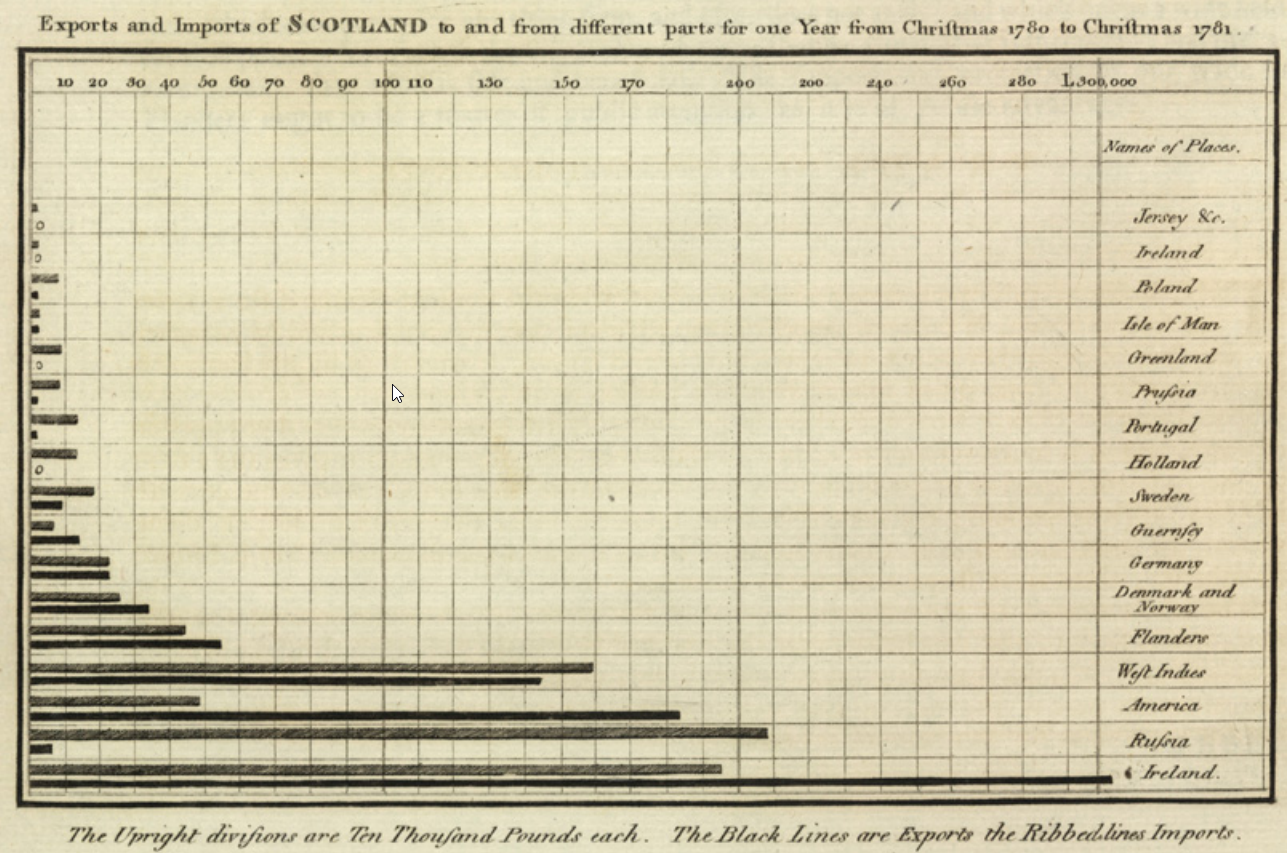
\includegraphics[keepaspectratio,width=\linewidth,height=\thirdh]
{images/playfair-bar-chart.png}
\caption[Bar Chart by William Playfair from 1786]{%
Bar chart of England's exports and imports to and from Scotland in
1781. Published in 1786, it is considered to be one of the
first occurrences of a bar chart containing most components found in
modern visualizations.
\imgcredit{Image extracted from Schoenberg Center
for Electronic Text and Image (SCETI).
Used under the terms of Creative Commons CC BY 2.5.}
}
\label{fig:PlayfairBarChart}
\end{figure}



\begin{figure}[tp]
\centering
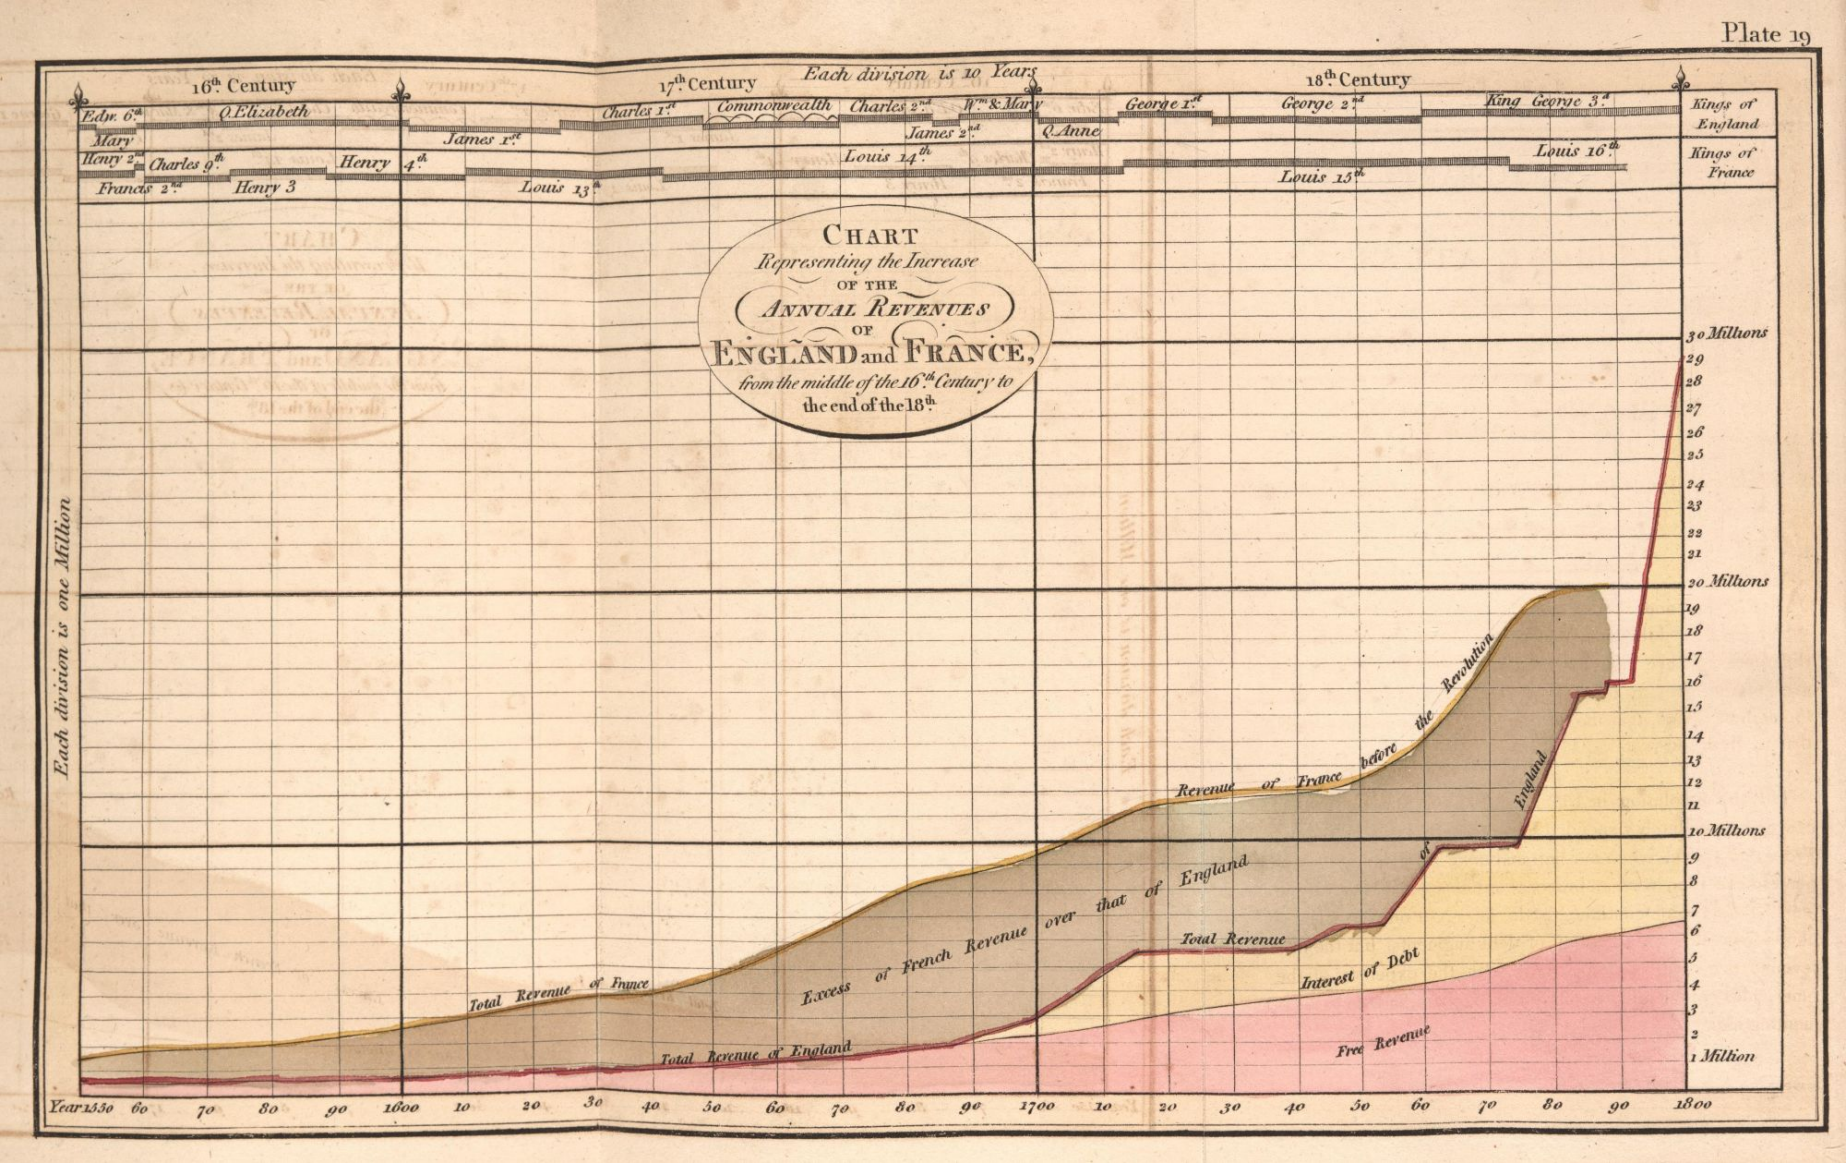
\includegraphics[keepaspectratio,width=\linewidth,height=\thirdh]
{images/playfair-area-chart.png}
\caption[Area Chart by William Playfair from 1786]{%
Area chart of annual revenues of England and France between
1550 and 1800. Published in 1786, it is considered to be one of
the first occurrences of an area chart
containing most components found in modern visualizations.
\imgcredit{Image extracted from Schoenberg Center
for Electronic Text and Image (SCETI).
Used under the terms of Creative Commons CC BY 2.5.}
}
\label{fig:PlayfairAreaChart}
\end{figure}




%% The dot map created by \textcite{ModeOfCommunicationOfCholera} in 1855
%% to trace cholera outbreaks in London (Figure~\ref{fig:CholeraDotMap})
%% is undoubtedly one of the most famous and influential visualizations
%% in history.  Even though it is not directly an information
%% visualization but rather a geographic one, it has been included here
%% because of its historic relevance.  This iconic dot map was used to
%% identify a cluster of cholera-related deaths near a contaminated water
%% pump on Broad Street, leading to the recognition of cholera as a
%% waterborne disease.
%% 
%% 
%% \begin{figure}[tp]
%% \centering
%% 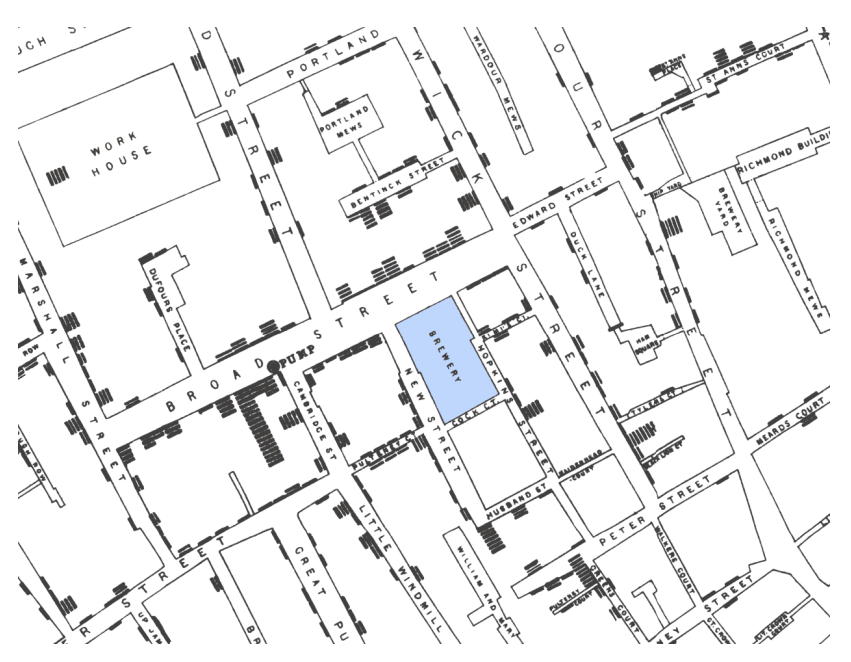
\includegraphics[keepaspectratio,width=\linewidth,height=\fullh / 3]{images/cholera-dot-map.png}
%% \caption[Dot Map Plotting Cholera Deaths in London From 1855]{%
%% This iconic chart was created by Dr. John Snow in 1855 to identify a
%% clustering of cholera-related deaths near Broad Street in London.  It
%% was used to identify a contaminated water pump and to illustrate the
%% waterborne nature of the disease.  Since the data is map-based, this
%% chart is an example of a geographic visualization rather than an
%% information visualization.
%% \imgcredit{Image extracted from \textcite{IVISCourseNotes}.
%% Original appearance in \textcite{ModeOfCommunicationOfCholera}.}
%% }
%% \label{fig:CholeraDotMap}
%% \end{figure}






It would be amiss not to mention Florence Nightingale (1820--1910)
\parencite{FlorenceNightingale} when talking about the history of
information visualization. She was a British statistician, social
reformer, and the founder of modern nursing and might be the first
person who used visualizations to persuade others of a need for
change. During her service as a superintendent of nurses in the
Crimean War, she realized that a large number of deaths in hospitals
resulted from preventable diseases which originated in poor sanitary
conditions. One of her contributions to the field of information
visualization was the creation of a new type of diagram, called a rose
diagram or polar-area chart, shown in
Figure~\ref{fig:NightingalePolarAreaChart}. She used these charts to
communicate data she collected on the mortality of soldiers during the
war and to grab the attention of politicians and the public.

\begin{figure}[tp]
\centering
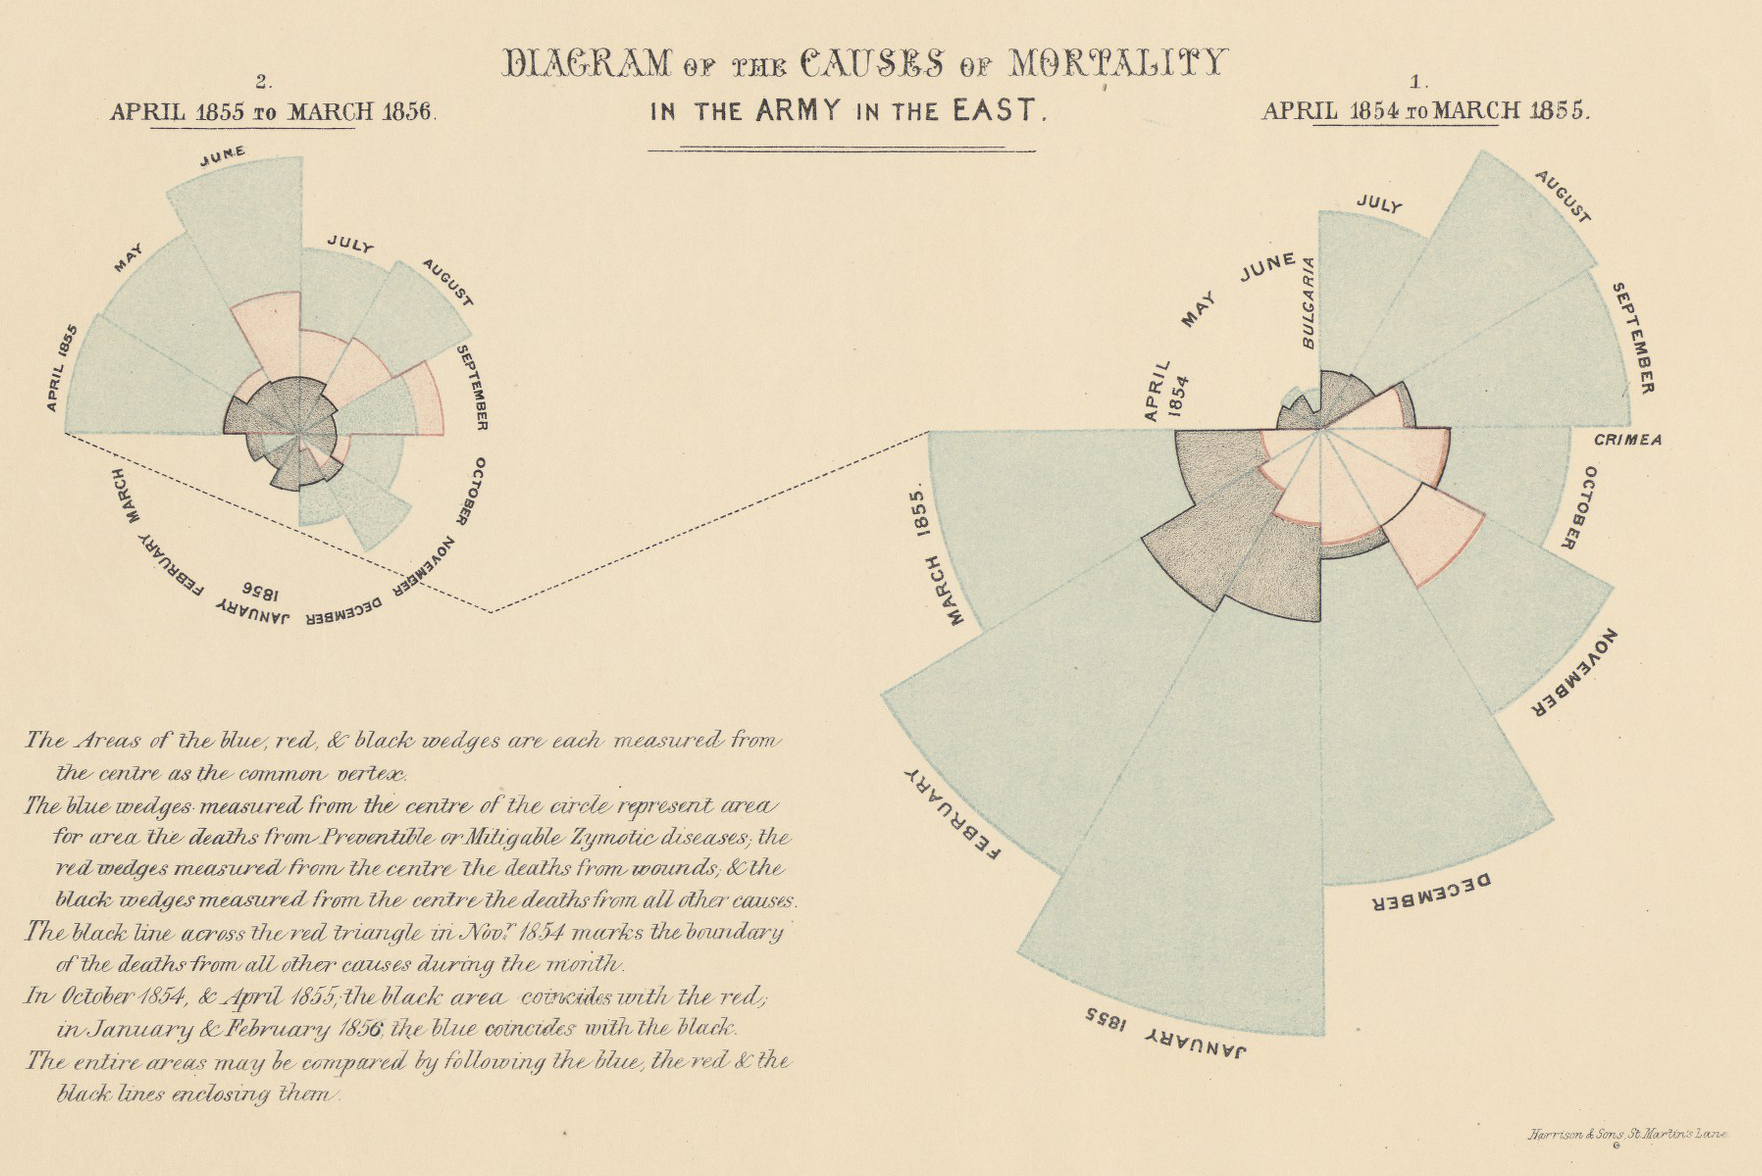
\includegraphics[keepaspectratio,width=\linewidth,height=\thirdh]
{images/nightingale.png}
\caption[Polar-Area Chart by Florence Nightingale from 1859]{%
One of the polar-area charts created by Florence Nightingale in 1859
to convince people of a need for more sanitary conditions in
hospitals. It visualizes the causes of mortality for soldiers during
the Crimean War and demonstrates that a large percentage of patients
died from preventable diseases linked to unsanitary environments.
\imgcredit{Image extracted from Harvard Library.
Used under the terms of Creative Commons Attribution 4.0.}
}
\label{fig:NightingalePolarAreaChart}
\end{figure}




Modern visualizations benefit from the interactive nature of the
devices used to consume them. They can be more complex than static
visualizations, because various interaction techniques enable users to
navigate large amounts of data and make sense of it. High-D by
Macrofocus \parencite{HighD} is a representative example of a modern
interactive visual analytics tool, and is shown in
Figure~\ref{fig:HighD}.

\begin{figure}[tp]
\centering
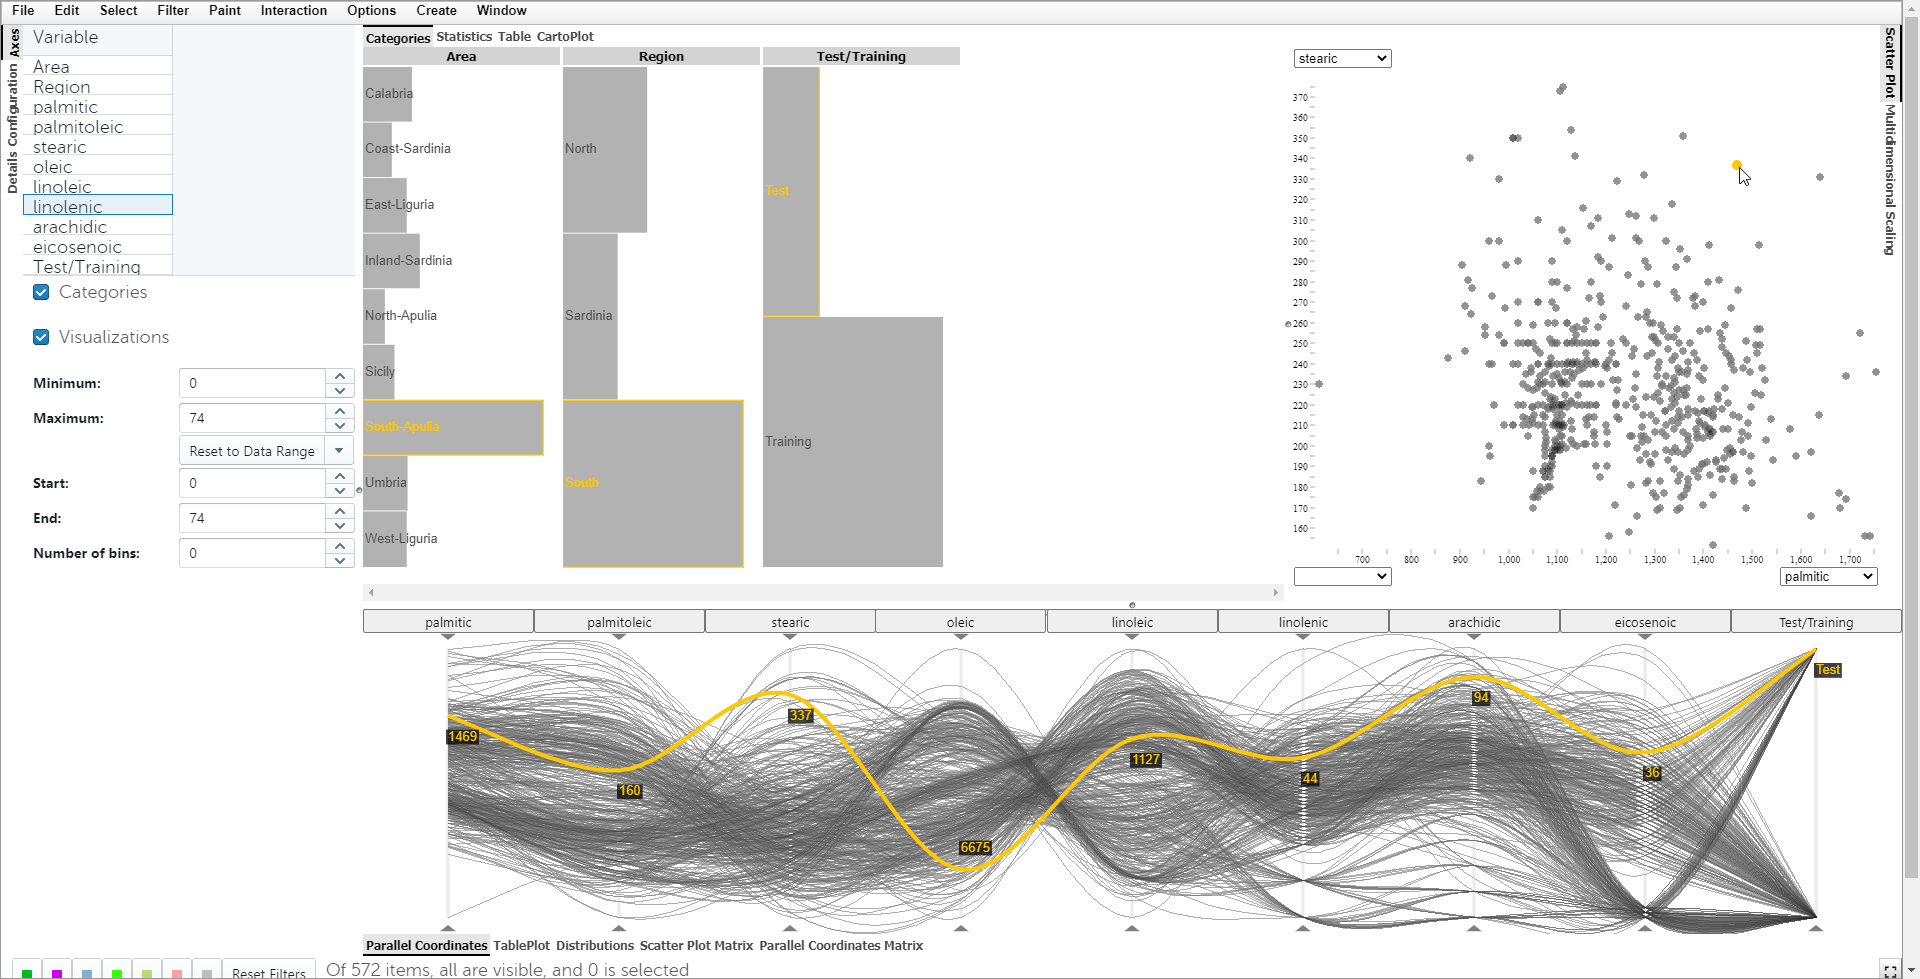
\includegraphics[keepaspectratio,width=\linewidth,height=\thirdh]
{images/high-d.png}
\caption[High-D]{
High-D by Macrofocus is a visual analytics tool
specialized in analyzing multidimensional data.
\imgcredit{Screenshot of High-D \parencite{HighD} taken by the author of this work.}
}
\label{fig:HighD}
\end{figure}




It is out of the scope of this work to provide a full account of the
long and eventful history of information visualization. This section
only provides a brief and very selective view of the topic.  More
comprehensive works for further reading include
\textcite{BriefHistoryOfDataVis}, \textcite{Meirelles-2013},
\textcite{HistoryOfInformationGraphics}, and
\textcite{HistoryOfDataVisAndGraphicCommunication}.










\section{Information Visualization Libraries for the Web}

There are many web-based libraries which simplify the rendering of
interactive visualizations. The approaches used to create and update a
visualization differ widely between libraries. D3 is a low-level
library which enables data-driven transformations of documents. Vega
and Vega-Lite provide a declarative grammar to express the visual and
interactive characteristics of a visualization. Template-based
visualization libraries provide a higher-level template-based
interface which can easily be configured.



\subsection{Data-Driven Documents (D3)}

D3 \parencite{D3} is a free, open-source document manipulation library
built in JavaScript by Mike Bostock and actively maintained by him and
a community on GitHub \parencite{D3JS}. Mike Bostock is also the
creator of Observable \parencite{Observable} and was one of the
authors of the now deprecated Protovis visualization library
\parencite{Protovis}. \textcite{Wattenberger-D3} is a great
introduction to D3.

D3 enables data-driven document transformations allowing developers to
describe documents as functions of data. As an example, developers can
define transformations which take a dataset and transform it into a
basic HTML table or into a more sophisticated visualization as an SVG
chart. This focus on explicitly defining transformations is well
suited to dynamic visualizations, because developers have complete
control over the creation, modification, and removal of elements. It
also sets D3 apart from other visualization libraries, where
developers define the desired state of a representation using a
declarative domain-specific language.

In contrast to other visualization libraries, D3 contains no
proprietary visual primitives and relies on well established web
standards like HTML, SVG, and CSS to implement its visual
representations. This yields great flexibility, because developers
work directly with web standards implemented in browsers and do not
need to wait for D3 to support for new features as standards
evolve. If developers chose to switch to a different library, the
knowledge of web standards gained during their work with D3 might be
applicable to their future work. The reliance on web standards also
makes it possible to use the native debugging tools available in web
browsers.


Other important aspects of D3's design include immediate evaluation of
functions, the principle of parsimony, and support for method
chaining. Immediate evaluate of functions means that operations, such
as modifying attributes, are applied instantaneously at the time of
calling the respective functions. This reduces internal complexity by
handing control flow decisions over to invoking code. It also avoids
errors related to missing state changes when state is modified
multiple times between rendering, which commonly occur in libraries
which use delayed evaluation of functions.

The principle of parsimony, also referred to as Occam's razor, is a
problem-solving principle which stems from the field of philosophy
\parencite{PrincipleOfParsimony}. It is frequently paraphrased as
\enquote{entities should not be multiplied beyond necessity}, and when
applied to API design it means that superfluous functions in an API
should be avoided. As an example, the background color of a circle
element can already be set with the generic \lstinline{Selection.attr}
method to set the \attrname{background-color} attribute of all
elements in a Selection. Adding an additional
\lstinline{backgroundColor} method would violate the principle of
parsimony because it would introduce a special method to achieve
something that was already achievable.

Method chaining is a popular syntax which allows functions to be
chained after one another. The use of method chaining avoids having to
store intermediate method results in variables which would not
otherwise be needed. It is implemented in D3 by returning the
\lstinline{Selection} on which a modifying method is called as a
result of that method. Methods which insert new elements into the DOM,
such as \lstinline{Selection.append} and \lstinline{Selection.insert},
return a Selection of the newly added elements to enable the creation
of nested structures. This method chaining syntax is further aided by
the \lstinline{Selection.call} method, which invokes a callback
receiving the current Selection as a parameter and returns the
original Selection to chain further methods on it after the callback
has been executed. The \lstinline{Selection.call} method enables the
creation of complex method chaining structures and is widely used by
developers. A simple example of method chaining in D3 with the
\lstinline{Selection.call} method can be seen in
Listing~\ref{list:D3MethodChaining}.



\begin{samepage}
\lstinputlisting[%
  float=tp,
  aboveskip=\floatsep,
  belowskip=\floatsep,
  xleftmargin=0cm,              % no extra margins for floats
  xrightmargin=0cm,             % no extra margins for floats
  %
  language=JavaScript,
  basicstyle=\footnotesize\ttfamily,
  frame=shadowbox,
  numbers=left,
  label=list:D3MethodChaining,
  caption={[D3 Method Chaining]%
A simple example of method chaining in D3.
A \elname{h1} element and a \elname{p} element are created
inside an existing \elname{body} element.
},
]{listings/d3-method-chaining.js}
\end{samepage}


Selections are the atomic building blocks of D3 and are used to access
almost any functionality.  Selections are created using the
\lstinline{d3.select} or \lstinline{d3.selectAll} methods.  These
methods are built on the \lstinline{querySelector} and
\lstinline{querySelectorAll} methods of the DOM Selectors API, which
allow the selection of elements via CSS selectors (see
Section~\ref{sec:CSS}). The \lstinline{d3.select} and
\lstinline{d3.selectAll} methods create a Selection containing either
a single element matching the provided selector, or multiple elements
matching it, respectively. A Selection acts as a wrapper container
around selected elements to perform frequently performed DOM
operations on them.  Among others, the element operations provided by
a Selection include the setting and getting of: attributes using the
\lstinline{Selection.attr} method, styles using the
\lstinline{Selection.style} method, properties using the
\lstinline{Selection.property} method, text or HTML content using the
\lstinline{Selection.text} or \lstinline{Selection.html} methods, and
event listeners using the \lstinline{Selection.on} method. Selections
also provide wrapper methods to insert additional elements using the
\lstinline{Selection.append} or \lstinline{Selection.insert} methods,
as well as to remove them using the \lstinline{Selection.remove}
method. Accessing the DOM via this wrapper is less tedious than
accessing it directly, because the native DOM API is very verbose, and
also because the method chaining API provided by D3 does not require
the storage of unnecessary intermediate variables.

An additional feature of D3 is the ability to bind data to elements
using the \lstinline{Selection.data} and \lstinline{Selection.datum}
methods. The \lstinline{Selection.datum} method binds a single
provided data record to all elements in the Selection, whereas the
\lstinline{Selection.data} method receives an array of data records
and binds each individual data record to exactly one element.  The
\lstinline{Selection.data} method performs a join operation between
data and elements to ensure that exactly one element per data record
exists. This data join results in three separate Selections: the enter
Selection, containing the elements which were newly created, the
update Selection, containing the elements which merely receive new
data, and the exit Selection, containing the elements which are being
removed. Each of these Selections can be individually transformed
using the \lstinline{Selection.join} method, which can receive three
callbacks for the enter, update, and exit Selections of the data join,
respectively. This ability to individually control changes to
entering, updating, and exiting elements is referred to in D3 as the
\emph{general update pattern}. A simple demonstration of how it is
used can be seen in Listing~\ref{list:D3GeneralUpdatePattern}. All the
previously mentioned DOM wrapper methods can receive either constant
values or dynamic values defined as functions. These functions receive
the bound element data, the element's index in the group of nodes
represented by the Selection, and the group of nodes themselves as
input and then calculate a dynamic value based on these parameters,
which is forwarded to the corresponding DOM method.


\begin{samepage}
\lstinputlisting[%
  float=tp,
  aboveskip=\floatsep,
  belowskip=\floatsep,
  xleftmargin=0cm,              % no extra margins for floats
  xrightmargin=0cm,             % no extra margins for floats
  %
  basicstyle=\footnotesize\ttfamily,
  frame=shadowbox,
  numbers=left,
  label=list:D3GeneralUpdatePattern,
  caption={[D3 General Update Pattern]%
A simple demonstration of D3's general update pattern being used to
specify different transformations for entering, updating, and exiting
elements. The full utility of this pattern is only apparent in more
complex scenarios involving transitions.
},
]{listings/d3-join.js}
\end{samepage}



D3 also offers a convenient, optional API to perform JavaScript-based
animations via Transitions, which wrap a Selection and allow the
animation of various element characteristics.  Transitions are created
using the \lstinline{Selection.transition} method which creates a
Transition wrapping the Selection on which it has been called.  The
duration of a Transition is defined using the
\lstinline{Transition.duration} method and its easing can be
configured using the \lstinline{Transition.ease} method. It is also
possibile to interrupt and chain transitions. Transitions provide an
almost identical API to Selections. The major change is that the
wrapping methods interpolate towards their target values using the
given easing function over the given duration instead of setting the
target value directly. Using D3 Transitions is completely optional and
developers can choose instead to use other animation technologies,
like CSS transitions and animations.

At its core, D3 is simply a low-level library to perform data-driven
document transformations. Even though this generic core technology is
applicable to a wide range of use cases, D3 was created with a focus
on creating visualizations. There are many additional modules which
simplify the higher-level tasks necessary for creating and rendering
visualizations. All D3 modules follow the same inherent patterns, like
method chaining and configurable functions. Therefore, despite this
higher-level functionality being split over multiple modules, a
consistent experience is provided to developers. Listing all available
modules here would be out of the scope of this work, but some
noteworthy modules include: \modname{d3-shape} to create visual
primitives like lines and areas, \modname{d3-scale} to encode abstract
data dimensions, \modname{d3-axis} to render scales as human-readable
axes, and many more such as \modname{d3-array}, \modname{d3-layout}
and \modname{d3-zoom}.
% KA add a short characterisation of d3-array, d3-layout, and d3-zoom







\subsection{Vega and Vega-Lite}

Vega \parencite{Vega} is a library consisting of a grammar to describe
interactive graphics and a parser which translates specifications
written in this grammar into static images or web-based views built on
SVG documents or the Canvas Web API. An interactive visualization in
Vega is fully described by a specification written in Vega's grammar.
This grammar is essentially a domain-specific language designed for
the declarative specification of interactive graphics. Its syntax is
based on the easy-to-read JavaScript Object Notation (JSON), which is
among the most frequently used textual serialization formats. Vega
builds on previous research in the field of declarative visualization
design \parencite{GrammarOfGraphics}. In contrast to previous work, it
contains powerful capabilities to declaratively describe interactions
\parencite{ReactiveVega} in addition to describing visual appearance.

The visual aspects of a visualization are described in a grammar
similar to the Grammar of Graphics defined by
\textcite{GrammarOfGraphics}. At its top level, a Vega specification
contains properties to configure sizing and padding of the container
of a visualization. Every specification also contains a data section,
which either defines data or specifies where to load it from.  The
Vega grammar also supports various forms of data transformation which
can successively be applied to a dataset to perform various
transformations like filtering, deriving additional fields, or
deriving additional datasets. In a majority of cases, the defined data
will consist of abstract information which is then mapped to visual
properties. This mapping is configured and performed using scales.
Vega already contains a variety of scales to help with mapping
abstract values to visual properties. They can broadly be categorized
into quantitative scales which map quantitative inputs to quantitative
outputs, discrete scales which map discrete inputs to discrete
outputs, and discretizing scales which map quantitative inputs to
discrete outputs. For spatially encoded dimensions, scales can
be visualized as axes, whereas non-spatial encodings such as encodings
as colors, sizes, or shapes can be visualized as legends.

At the core of every visualization lies the encoding of data as visual
primitives, which is achieved in Vega via marks. Marks use scales to
encode data fields as properties of their shapes. Based on the general
update pattern of the underlying D3 library, the encoding of marks can
be separately controlled for newly created (entering) marks, existing
and not exiting (updating) marks, and to-be-removed (exiting)
marks. In addition to these basic visualization components, the Vega
grammar contains further capabilities to describe interactions (via
signals, triggers, and event streams), cartographic projections,
sequential or layered views (via mark groups), layouts, and color
schemes. To demonstrate how the various aspects of a Vega
specification are defined, an example of a static bar chart can be
seen in Listing~\ref{list:VegaStaticBarChart}.


\begin{samepage}
\lstinputlisting[%
  float=tp,
  aboveskip=\floatsep,
  belowskip=\floatsep,
  xleftmargin=0cm,              % no extra margins for floats
  xrightmargin=0cm,             % no extra margins for floats
  %
  basicstyle=\footnotesize\ttfamily,
  frame=shadowbox,
  numbers=left,
  label=list:VegaStaticBarChart,
  caption={[Static Bar Chart in Vega]%
The Vega specification of a static bar chart.
It demonstrates the use of data, scales, axes, and marks
to construct the bar chart.
},
]{listings/vega-static-bar-chart.json}
\end{samepage}


In template-based visualization libraries, interactions are typically
defined by configuring premade interaction templates, which is easy
but limiting, or by manually modifying the visualization in various
callbacks, which is flexible but tedious and not serializable. The
ability to describe custom interactions using a serializable,
data-driven grammar is what sets Vega apart from other declarative
visualization librarie \parencite{ReactiveVega}. This approach offers
the flexibility of callback-driven interactions, while still remaining
fully serializable and declarative. The grammar to define interactions
is based on the syntax of event-driven functional reactive programming
\parencite{EventDrivenFRP}, a high-level grammar which resembles
mathematical equations to describe reactive systems. In Vega, the
primitives to express interactions are called \emph{signals}. Signals
can be seen as dynamic variables which change their values based on
input events or other signals. These signals and the way their values
change are defined declaratively, and they can be used as dynamic
variables in most places in a Vega specification to change various
characteristics of a visualization dynamically.
Listing~\ref{list:VegaBarChart} shows an example of how the previously
shown static bar chart specification can be extended with signals to
display a tooltip when hovering over bars.



\begin{samepage}
\lstinputlisting[%
  float=tp,
  aboveskip=\floatsep,
  belowskip=\floatsep,
  xleftmargin=0cm,              % no extra margins for floats
  xrightmargin=0cm,             % no extra margins for floats
  %
  basicstyle=\footnotesize\ttfamily,
  frame=shadowbox,
  numbers=left,
  label=list:VegaBarChart,
  caption={[Bar Chart with Tooltip in Vega]%
The necessary additions to the static bar chart specification in
Listing~\ref{list:VegaStaticBarChart} to display a tooltip when
hovering over bars. It demonstrates the basic functionality of signals
in Vega. When the mouse hovers over a \elname{rect} mark, the tooltip
signal will receive the value of the \elname{rect}'s bound data
record. The \elname{tooltip} signal will be reset to an empty object when the
mouse leaves the \elname{rect} mark. It is then used in the newly
added \elname{text} mark section of the specification to define the
position, text, and visibility of the tooltip whenever an update
occurs.
},
]{listings/vega-bar-chart.json}
\end{samepage}



Visualizations created with Vega closely follow their specifications
and minimal assumptions are made in the compilation process. This
results in very verbose specifications, because all configurations for
all parts of the visualization need to be explicitly defined in them.
It also means that specification authors have full control over the
resulting graphics, making Vega a good base on which to build further
libraries and tools. Many tools have already been built on top of Vega
\parencite{Voyager,Lyra,CompassQL}. Most noteworthy is Vega-Lite
\parencite{VegaLite}. Vega-Lite is described as a \enquote{high-level
  grammar of interactive graphics}, which summarizes its difference to
Vega fairly well. Vega-Lite is a higher-level grammar than Vega,
allowing authors to write specifications for common visualizations in
a much more concise form. Specifications written in Vega-Lite are then
compiled into Vega specifications. During compilation, the compiler
automatically derives default configurations for axes, legends, and
scales by following a set of carefully designed rules. This makes
Vega-Lite more convenient for quick authoring of visualizations, since
many of the details which need to be explicitly stated in a Vega
specification can be omitted. In those cases where the derived default
configurations are not suitable, Vega-Lite also offers the possibility
to override them. Since Vega-Lite specifications are simply compiled
into Vega ones, it is a sensible choice to use Vega-Lite as a primary
tool to describe visualizations, and switch to Vega for more exotic
cases which are not easily achievable in Vega-Lite. To illustrate the
difference between a Vega and a Vega-Lite specification,
Listing~\ref{list:VegaLiteBarChart} shows a Vega-Lite version of the
Vega bar chart specification from
Listings~\ref{list:VegaStaticBarChart} and~\ref{list:VegaBarChart}
combined.


\begin{samepage}
\lstinputlisting[%
  float=tp,
  aboveskip=\floatsep,
  belowskip=\floatsep,
  xleftmargin=0cm,              % no extra margins for floats
  xrightmargin=0cm,             % no extra margins for floats
  %
  basicstyle=\footnotesize\ttfamily,
  frame=shadowbox,
  numbers=left,
  label=list:VegaLiteBarChart,
  caption={[Bar Chart with Tooltip in Vega-Lite]%
A Vega-Lite specification of the Vega bar chart shown in
Listings~\ref{list:VegaStaticBarChart} and~\ref{list:VegaBarChart}
combined.
},
]{listings/vega-lite-bar-chart.json}
\end{samepage}








\subsection{Template-Based Visualization Libraries}

Template-based visualization libraries work by providing templates for
possible types of visualizations and allowing users to customize them.
These types of visualization libraries are easier to use than D3 or
Vega because they offer a concise form of configuration which does not
require users to have detailed knowledge over the underlying rendering
technology or complex, non-standardized domain specific languages.
Even though these types of libraries are usually flexible enough to
create a huge range of visualizations, at some point users may run
into limitations. Some of these limitations can only be worked around
by writing custom source code, which requires a deep understanding of
the underlying library. This effectively eliminates the ease-of-use
benefit of these types of libraries for users who run into these
limitations.

For this thesis, a total of 20 template-based JavaScript visualization
libraries were examined and compared according to factors such as
their rendering technology, usage popularity (number of downloads),
open-source popularity, license, and recent development activity.  In
terms of rendering technology, most libraries render visualizations as
either SVG documents or canvas elements, although some implement a
hybrid renderer which can be configured to render as either one of
them. Usage popularity was measured by the cumulative package
downloads from the npm package manager over the previous twelve
months. This was deemed one of the most relevant metrics for the
comparison, because it reflects actual user behavior and gives an
indication on how widespread a library is used in practice. The 20
libraries found in the initial collection phase were filtered by their
usage popularity and recent development activity to remove those which
were not sufficiently used or no longer maintained. This filtering
step yielded the following ten libraries: (1) ChartJS
\parencite{ChartJS}, (2) Highcharts \parencite{Highcharts}, (3)
ECharts \parencite{ECharts}, (4) ApexCharts \parencite{ApexCharts},
(5) PlotlyJS \parencite{PlotlyJS}, (6) C3JS \parencite{C3JS}, (7)
Chartist \parencite{Chartist}, (8) amCharts \parencite{amCharts}, (9)
billboardJS \parencite{billboardJS}, and (10) D3FC \parencite{D3FC}.
These ten libraries were selected for further consideration.

Eight of the ten libraries are completely free to use without
restrictions, amCharts has a free license for users who are
comfortable with an attribution logo on their visualizations, and
Highcharts offers a free license option for non-profit, educational
and personal applications. Nine of the libraries implement an
SVG-based renderer, two of which (ECharts and D3FC) also offer
alternative rendering to Canvas elements for high-performance
scenarios, and only ChartJS solely targets canvas-based rendering.
Eight libraries are very actively maintained with most of them showing
development activity within the last month. C3JS and Chartist seem to
be no longer actively maintained, but were included nontheless in the
deeper evaluation, due to their historic and thematic relevance and
because they are still widely used.

Template-based visualization libraries have a strong inclination
towards designing their APIs according to principles of declarative
programming.  APIs following these principles allow users to describe
a desired state they want the underlying system to be in.  This is in
strong contrast to the typical imperative way of designing APIs in
which users are instead given a set of tools to query and modify a
system's state. The difference can be summarized in simple terms as
follows: With declarative APIs, users specify what state shall be
achieved, whereas with imperative APIs, users specify how a certain
state is achieved. Declarative APIs are typically built on top of
lower-level imperative APIs and can therefore be seen as a higher
level of abstraction over them. They are popular among developers
because they are expressive, easy to use and effectively encapsulate
complexity which would otherwise have to be handled by users. An often
overlooked disadvantage of declarative APIs is that they frequently
only provide high-level access to a system and that more specific use
cases might not be achievable if they can not be expressed in the
domain-specific language defined by the API. In many cases, it makes
sense to provide additional imperative APIs for users which require a
lower level of access to the system to implement functionality not
achievable via the declarative parts of the interface.

All of the evaluated libraries, except D3FC, expose declarative
interfaces in the form of nested configuration objects which are used
to specify the characteristics of individual visualizations. Apart
from Chartist, all those libraries feature generic high-level creation
functions. These functions create charts from declarative
configuration objects, which allow the specification of different
forms of visualization for different data dimensions. This type of
interface is demonstrated by the Highcharts code in
Listing~\ref{list:Highcharts}. Generic chart creation functions seem
to correlate with the ability to dynamically change the type of
visualization. Chartist, on the other hand, provides separate chart
creation functions for each type of chart, and it is not possible to
alter the type of chart after it has been created. Another limitation
which may originate from partitioning the API by chart type is that
mixed charts which combine multiple forms of visualization in one
composite visualization cannot be expressed.


\begin{samepage}
\lstinputlisting[%
  float=tp,
  aboveskip=\floatsep,
  belowskip=\floatsep,
  xleftmargin=0cm,              % no extra margins for floats
  xrightmargin=0cm,             % no extra margins for floats
  %
  basicstyle=\footnotesize\ttfamily,
  frame=shadowbox,
  numbers=left,
  label=list:Highcharts,
  caption={[Bar Chart in Highcharts]%
A basic column (vertical bar) chart defined using Highcharts' generic
chart creation API. A high-level, declarative configuration object is
passed to the creation function.
},
]{listings/highcharts.js}
\end{samepage}



The only library in the deeper evaluation which does not provide a
high-level declarative configuration API is D3FC.  The design
philosophy of D3FC is based on the idea of \enquote{unboxing} D3.
Even though many visualization libraries are implemented on top of D3,
it is usually hidden behind public APIs which are easier to work with
but do not provide the full flexibility of D3. D3FC exposes a
component-based interface which closely follows design patterns
frequently encountered when working with D3. These components form
higher-level building blocks upon which advanced visualizations can be
built. They are also highly configurable and in those cases where the
options for configuration are not sufficient, a decorator pattern is
allows users to hook into the underlying D3 functionality and inject
custom code into the various stages of the general update pattern at
the core of D3. Code demonstrating the usage of D3FC can be seen in
Listing~\ref{list:D3FC}.


\begin{samepage}
\lstinputlisting[%
  float=tp,
  aboveskip=\floatsep,
  belowskip=\floatsep,
  xleftmargin=0cm,              % no extra margins for floats
  xrightmargin=0cm,             % no extra margins for floats
  %
  basicstyle=\footnotesize\ttfamily,
  frame=shadowbox,
  numbers=left,
  label=list:D3FC,
  caption={[Bar Chart in D3FC]%
A basic bar chart defined using D3FC's component-based API.
},
]{listings/d3fc.js}
\end{samepage}



amCharts is the only evaluated library, which exposes a hybrid API
with the possibility of configuring visualizations using both
declarative configuration objects and manually composing higher-level
visualizations from lower-level components, such as axes and series.
Its component-based interface is still rather declarative, with most
options being configurable by modifying specific properties on the
components. However, modifying only the properties which require
changing instead of processing a full configuration object and
figuring out the necessary changes from it, is less costly in terms of
performance. In addition to these performance benefits, the components
provide additional functions to perform operations which would not be
available using a purely declarative API.




When comparing the evaluated libraries in terms of their responsive
configurability, most libraries offer similar capabilities albeit in
slightly different ways. Six of the ten libraries (Highcharts, C3JS,
Chartist, amCharts, billboardJS, and D3FC) support the styling of
elements in their created visualizations with CSS, which requires
rendering as SVG documents, since only document-based visualizations
can be affected by CSS. The styling of visualizations with CSS is
powerful, because it leads to a separation of concerns and designers
can make use of CSS-inherent mechanisms to configure responsive
styles.  Unfortunately, CSS-based styling is only of limited
applicability because not all CSS properties affect SVG elements, as
described in Section~\ref{sec:SVG}.
% KA  not sure about this last sentence??

To responsively configure other visualization characteristics, such as
their type, data, and layout, designers have to resort to
configuration mechanisms offered by the libraries. Four libraries
(Highcharts, ApexCharts, Chartist, and amCharts) provide the
possibility to specify rule-based responsive configurations as part of
their declarative interfaces, illustrated in the Highcharts example in
Listing~\ref{list:HighchartsResponsive}. These declarative rules
consist of a condition part which specifies when to apply the rule,
and a configuration part which specifies the configuration options
which should be set when applying the rule. Even though this is a
convenient form of responsive configuration, if the desired conditions
can not be expressed via the provided declarative properties,
designers have to fall back to more generic mechanisms which are also
applicable to other libraries. The mechanisms for responsive
configuration in the other libraries are more generic, because they do
not offer these configurations as part of their declarative
interfaces. This means that developers need to trigger responsive
configurations themselves by manually reconfiguring visualizations via
their APIs in custom resize or media query event listeners. Nearly all
libraries provide a means to dynamically resize visualizations and
update their data, type, and options. The exceptions are
C3JS, which only supports dynamic changes of some options, and
Chartist, which does not support changing a visualization's type at all.



\begin{samepage}
\lstinputlisting[%
  float=tp,
  aboveskip=\floatsep,
  belowskip=\floatsep,
  xleftmargin=0cm,              % no extra margins for floats
  xrightmargin=0cm,             % no extra margins for floats
  %
  basicstyle=\footnotesize\ttfamily,
  frame=shadowbox,
  numbers=left,
  label=list:HighchartsResponsive,
  caption={[Responsive Rules in Highcharts]%
The declaration of responsive rules in Highcharts. In this example,
the x-axis and y-axis titles are removed if the chart is narrower than
500 pixels.
},
]{listings/highcharts-responsive.js}
\end{samepage}

% KA  Is the value in pixels?  How about ems?


          

\cleardoublepage

\chapter{Responsive Information Visualization}
\label{chap:ResponsiveInformationVisualization}

A \emph{responsive} visualization is a visualization which adapts
itself to the available display space and characteristics of the
device used to access it. Analogous to responsive web design, the need
for responsive visualizations arises from the growing variety of
devices used to consume content and the physical differences between
them.  Visualizations and charts often form significant blocks of
content embedded inside web pages. For a web page to be responsive,
any embedded content such as visualizations and charts must also be
responsive.

Visual elements require proper sizing and spacing to be of value.
Merely scaling visualizations to fit into their allocated space is
insufficient to provide a seamless experience to visualization
consumers, as has already been discussed in Section~\ref{sec:RWD}.
Even more elaborate automated visualization scaling techniques
\parencite{ViSizer, MobileVisFixer, SemanticResizing} only lead to
minor improvements compared to the more laborious approach of manually
adapting a visualization's design. Another factor which is often
ignored is the different methods of interaction inherent to specific
types of devices, such as touch and keyboard interaction. For example,
to ensure that data points remain selectable on less precise input
devices such as touchscreens, a visualisation might adapt by reducing
the data density and increasing the size of individual elements. The
goal of responsive visualizations is that they should adapt themselves
to the characteristics of the consuming device and context so as to
remain as effective and usable as possible
\parencite{DesignPatternsTradeOffsRespVis}.


The topic of responsive visualization only gained prominence in recent
years, as responsive web design became mainstream.
\textcite{BuildingRespDataVisForTheWeb} used the term responsive
visualization, but only descibed how to implement scalable
visualizations. \textcite{LearningRespDataVis} covered scalable
visualizations, but also considered interactive selection and touch
events. The work by Andrews
\parencite{RespVisTalk,RespVisPage,RespVis} was possibly the first
academic work to address design patterns for responsive visualization.
%
More recently, \parencite{TechniquesForFlexibleRespVisDesign} surveyed
the design space of responsive visualizations, created a taxonomy of
currently used techniques and recurring patterns, and presented a tool
to help design responsive visualisations side-by-side. In addition to
surveying design patterns, \textcite{DesignPatternsTradeOffsRespVis}
also consider issues around different forms of \enquote{message loss}
when reducing chart complexity, and define optimization of the
density-message trade-off as one of the main challenges when designing
responsive visualizations.


\textcite{Horak-2021-Responsive-Vis} is a recent and quite complete
summary of research in the field of responsive visualization. It
discusses the differences between responsive web design and responsive
visualization design and stresses that visualizations must not be seen
as mere images embedded in a website, but that they must adapt to
device characteristics to deliver a satisfactory visualization
consumer experience. Further, \textcite{Horak-2021-Responsive-Vis} go
into details about various factors affecting a visualization's
responsive design and give an overview of high-level design strategies
(called design patterns in this work) for responsive
visualizations. Lastly, unique challenges and opportunities for
responsive visualization design are summarized to guide researchers to
potentially interesting topics for future research in this area.





\section{Responsive Visualization Patterns}

Patterns are templates for solving recurring problems.
\textcite{TechniquesForFlexibleRespVisDesign} created a comprehensive
taxonomy of responsive techniques, as well as a tool to help design
responsive visualisations side-by-side. They proposed describing
responsive techniques according to five \emph{actions}, which are
applied to different components. These actions are: (1) resize, (2)
reposition, (3) add, (4) modify and (5) remove. A sixth action refers
to leaving a component unchanged, but this is deemed a non-technique
and therefore left out here. They also described a non-exhaustive set
of eleven \emph{components}, upon which these actions can be
performed: (1) axis, (2) axis labels, (3) axis ticks, (4) gridlines,
(5) legend, (6) data, (7) marks, (8) labels, (9) title, (10) view, and
(11) interaction. It should be noted that some combinations of actions
and components do not make sense and therefore do not occur in
practice. It is, for example, not possible to resize interactions or
reposition data. \textcite{TechniquesForFlexibleRespVisDesign}
performed their research following a desktop-first approach of
responsive design, because the interviews they conducted with
visualization authors revealed a strong inclination towards this
approach. They found that when adapting desktop visualizations for
narrow screens, it was much more common to remove elements (37.7\%)
than to add them (11.3\%). Another interesting finding was that most
visualizations (88.7\%) implemented no change at all for their
interactions, while some (10\%) even removed interactive capabilities
completely. Only very few visualizations (5.6\%) improved the
experience of mobile visualization consumers by adapting interactions
accordingly.



\begin{table}[tp]
\tablestretch
\rowcolors{2}{}{tablerowcolour}
\centering
\begin{tabularx}{\linewidth}{>{\kern-\tabcolsep}l>{\raggedright}p{0.2\textwidth}X<{\kern-\tabcolsep}}
\toprule
Category & Targets & Description \\
\midrule
Data        & Record, Field, Level &
Data apects such as records (rows), fields (columns), and level (of aggregation or hierarchy).\\
Encoding    & &
Visual representation in large-screen view. \\
Interaction & Feature, Trigger, Feedback &
Supported interactions in large-screen view. \\
Narrative   & Sequencing, Annotations, Emphases, Text &
Narrative, story-telling elements in large-screen view. \\
References / Layout & Labels, References, Layout, Size &
Additional elements such as labels and legends, and
placement of visual components in large-screen view. \\
\bottomrule
\end{tabularx}
\caption[Targets of Responsive Visualization Patterns]{
The targets of responsive visualization patterns identified by
\textcite{DesignPatternsTradeOffsRespVis}.
\imgcredit{Table adapted from \textcite{DesignPatternsTradeOffsRespVis}.}
}
\label{tab:PatternsTargets}
\end{table}



The most detailed research on patterns in responsive visualization
design was performed by \textcite{DesignPatternsTradeOffsRespVis}.
Following \textcite{TechniquesForFlexibleRespVisDesign}, they
characterised the responsive visualization strategies according to
(the same) two dimensions: \emph{targets}, representing what entity is
changed from large-screen to small-screen view, and \emph{actions},
representing how entities are changed. However, the targets and
actions are more finely grained, having a number of sub-categories.
%
Targets are grouped into five distinct categories (Data, Encoding,
Interaction, Narrative, and References/Layout), with four of the five
categories further divided into sub-categories, as shown in
Table~\ref{tab:PatternsTargets}.
%
Actions are also grouped into five distinct categories (Recompose,
Rescale, Transpose, Reposition, and Compensate), with four of the five
top-level categories again having sub-categories, as shown in
Table~\ref{tab:PatternsActions}. The actions are defined as operations
with distinct input and output states to ensure they can be inverted,
and thus can be applied to either desktop-first or mobile-first design
approaches
%
Categorizing techniques using these dimensions, the authors identified
a total of 76 viable strategies, whereby some of them are not used in
the visualizations they studied. Their explorable online gallery
\parencite{DesignPatternsTradeOffsRespVisGallery} contains examples
demonstrating all the patterns they discovered.



\begin{table}[tp]
\tablestretch
\rowcolors{2}{}{tablerowcolour}
\centering
\begin{tabularx}{\linewidth}{>{\kern-\tabcolsep}l>{\raggedright}p{0.35\textwidth}X<{\kern-\tabcolsep}}
\toprule
Category   & Actions & Description \\
\midrule
Recompose  & Remove, Add, Replace, Aggregate &
Actions affecting the existence of targets. \\
Rescale    &  &
Actions affecting the size of targets. \\
Transpose  & Serialize, Parellelize, Axis-Transpose &
Actions affecting the orientation of targets. \\
Reposition & Externalize, Internalize, Fix, Fluid, Relocate &
Actions affecting the position of targets. \\
Compensate & Toggle, Number &
Actions compensating for loss of information. \\
\bottomrule
\end{tabularx}
\caption[Actions of Responsive Visualization Patterns]{%
The actions of responsive visualization patterns identified by
\textcite{DesignPatternsTradeOffsRespVis}.
\imgcredit{Table adapted from \textcite{DesignPatternsTradeOffsRespVis}.}
}
\label{tab:PatternsActions}
\end{table}







\section{Responsive Visualization Examples}

The goal of this section is to provide the reader with some
demonstrative examples of responsive visualizations. Due to the
complexities of using images from commercial websites, the figures in
this section were taken from external academic sources from which
permissions are more straightforward to procure. These responsive
visualizations put most of their effort into demonstrating responsive
patterns rather than communicating messages in their data, and owing
to this, some of them lack essential features, such as chart and axis
titles, usually present in practice. For more real-life examples of
responsive visualizations,
\textcite{DesignPatternsTradeOffsRespVisGallery} should be consulted.

The examples in this section are organized by chart type. It would be
an immense endeavor to collect examples for every pattern used for all
types of charts, so only a subset demonstrating some of the most
frequently encountered patterns for frequently used types of charts is
presented here. The popularity of chart types was judged using the
responsive visualization corpus collected in
\textcite{DesignPatternsTradeOffsRespVisGallery} and the visualization
corpora from the Quarz news website and academic papers collected by
\textcite{ReverseEngineeringVisualizations}. Both of these sources
lead to the conclusion that line charts, bar charts, and point charts
are the most frequenly occuring types of visualizations.





\subsection{Bar Charts}
\label{sec:BarChartExamples}

Bar charts are usually used to visualize two-dimensional data, with
one categorical dimension and one quantitative dimension. Two variants
of bar charts support the visualization of categorical datasets having
subdimensions: grouped bar charts \parencite{GroupedBar} compare
subdimensions with each other, and stacked bar charts
\parencite{StackedBar} compare part-to-whole relationships of the
subdimensions. Even though responsive design of visualizations is
slowly becoming more common, most charts found in today's web articles
are still created as static images
\parencite{HBar,VBar,HVBar,MapBarLine}.

A good example of a responsive bar chart can be seen in
Figure~\ref{fig:RespBarExample} \parencite{RespVis}. Bar charts are
freely scalable by adjusting the width of individual bars
\parencite{RespHBar,RespHBarHLine,RespHBars}, so they all can fit into
their allocated space. When reducing the width of any type of chart
past a certain point, the tick labels of the horizontal axis may start
to overlap. This is why the reducing width pattern usually occurs
together with the recompose axis ticks and simplify/elaborate axis
labels patterns \parencite{RespHBars,RespHBarHLine,RespVBar}. Another
effective pattern for avoiding overlapping tick labels is to rotate
the labels by up to 90 degrees so they take up less horizontal space
\parencite{RespVis}. If there is too much data to fit into the
available width, the chart can be transposed and grown to as much
height as is required necessary \parencite{RespVis}. Doing this is
more advisable than simply extending the width of the chart past the
viewport, since vertical scrolling is easier than horizontal
scrolling. When reducing the width of charts containing annotations, a
number of patterns can be applied to avoid annotations
overlapping. For example, annotations can be removed
\parencite{RespHStackedBar,RespHLineHStackedBar}, simplified, or
relocated \parencite{RespVBar}.



\begin{figure}[tp]
\newlength{\respbarwidth}
\setlength{\respbarwidth}{0.95mm}
\centering
\subfloat[][%
70rem
]
{%
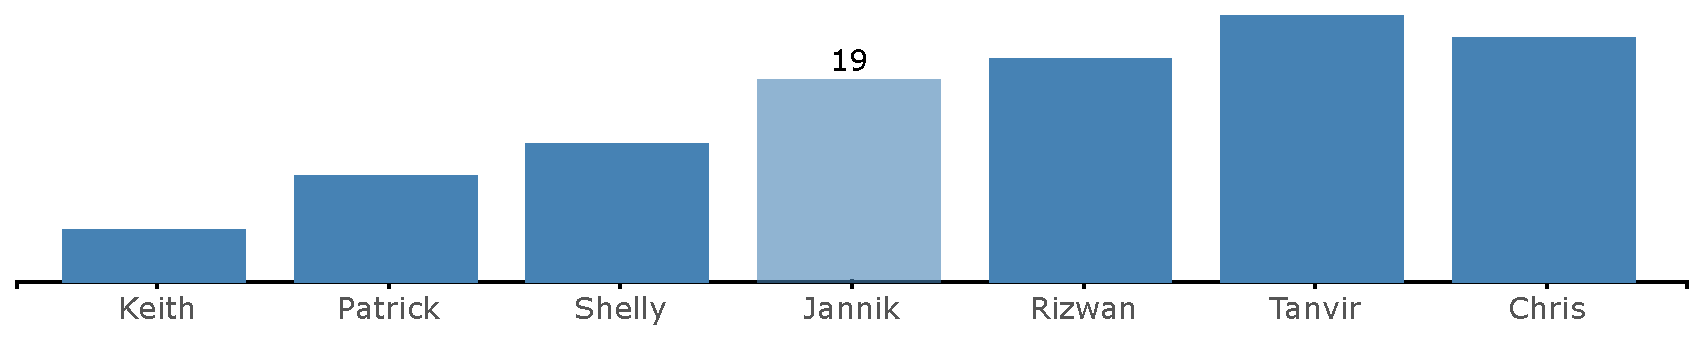
\includegraphics[width=70\respbarwidth]
{diagrams/resp-bar-1.pdf}%
\label{fig:RespBarExample1}%
}
\hfill
\subfloat[][%
50rem
]
{%
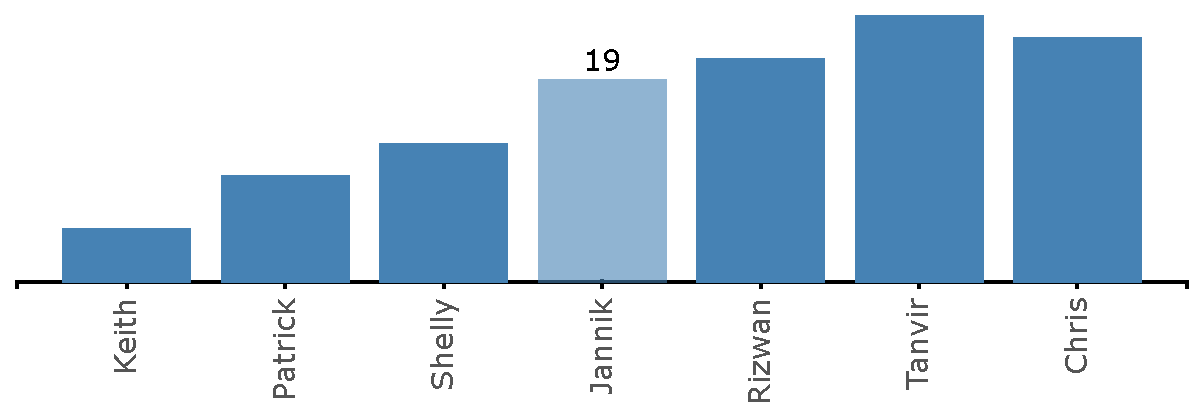
\includegraphics[width=50\respbarwidth]
{diagrams/resp-bar-2.pdf}%
\label{fig:RespBarExample2}%
}
\hfill
\subfloat[][%
30rem
]
{%
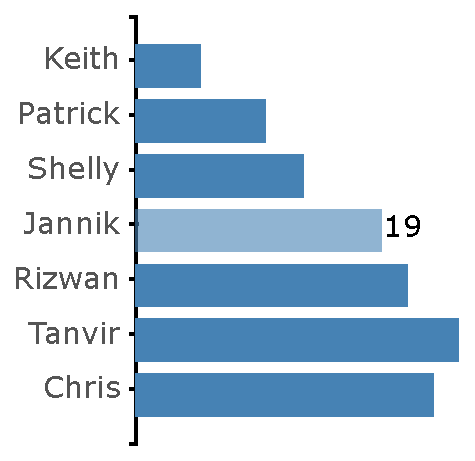
\includegraphics[width=30\respbarwidth]
{diagrams/resp-bar-3.pdf}%
\label{fig:RespBarExample3}%
}
\caption[Responsive Bar Chart Example]
{
A responsive bar chart at different display widths.
\subref{fig:RespBarExample1} At 70rem, axis tick labels are aligned
horizontally. \subref{fig:RespBarExample2} At 50rem, axis tick labels
are aligned vertically. \subref{fig:RespBarExample3} At 30rem, the
chart is transposed.
\imgcredit{Screenshots of \textcite{RespVisPage} created by the author of
  this thesis. Used with kind permission by Keith Andrews.}
}
\label{fig:RespBarExample}
\end{figure}






\subsection{Line Charts}
\label{sec:LineChartExamples}

Line charts are used to show trends in two-dimensional
datasets by plotting them as points connected by lines (a polyline).
They can be extended to compare trends in an additional categorical
dimension by drawing additional polylines for each category. Many line
charts on the web are published in non-responsive forms
\parencite{HLine,HLine2}, although some authors take the extra effort
to make their charts responsive. The minimum which can be done to make
a line chart responsive is to reduce their width
\parencite{RespRadialScatterHLine} on narrower screens by shrinking
the horizontal distance between neighboring points. This usually
occurs together with the recomposition and simplification of
horizontal ticks. If the chart contains annotations, it may also be
necessary to recompose, relocate, and simplify them as well
\parencite{RespHLines,RespHLine,RespHBarHLine,RespHLineHStackedBar}.

A good demonstration of which responsive patterns can be applied to
make a line chart responsive is shown in the responsive line chart
created by \textcite{RespVis} which can be seen in
Figure~\ref{fig:RespLineExample}. In addition to the recomposition of
ticks, tick labels are rotated to reduce their required horizontal
space. For exceptionally limited space, it can make sense to remove
the axes of a line chart entirely, turning it into a sparkline.
However, it should be noted that by doing this, the consumer of the
visualization loses information about the type and scale of the
chart's dimensions. This technique should therefore only be applied in
cases where no other pattern is applicable or if the trend in the data
is the most important message to convey. It is rare to encounter
transposed versions of line charts, although transposition could
sometimes benefit heavily annotated line charts \parencite{VLine}.
Applying a transpose pattern would allow the chart to take up as much
vertical space as necessary to neatly accomodate annotations without
requiring the consumer to scroll horizontally.



\begin{figure}[tp]
\newlength{\resplinewidth}
\setlength{\resplinewidth}{1.15mm}
\centering
\subfloat[][%
65rem
]
{%
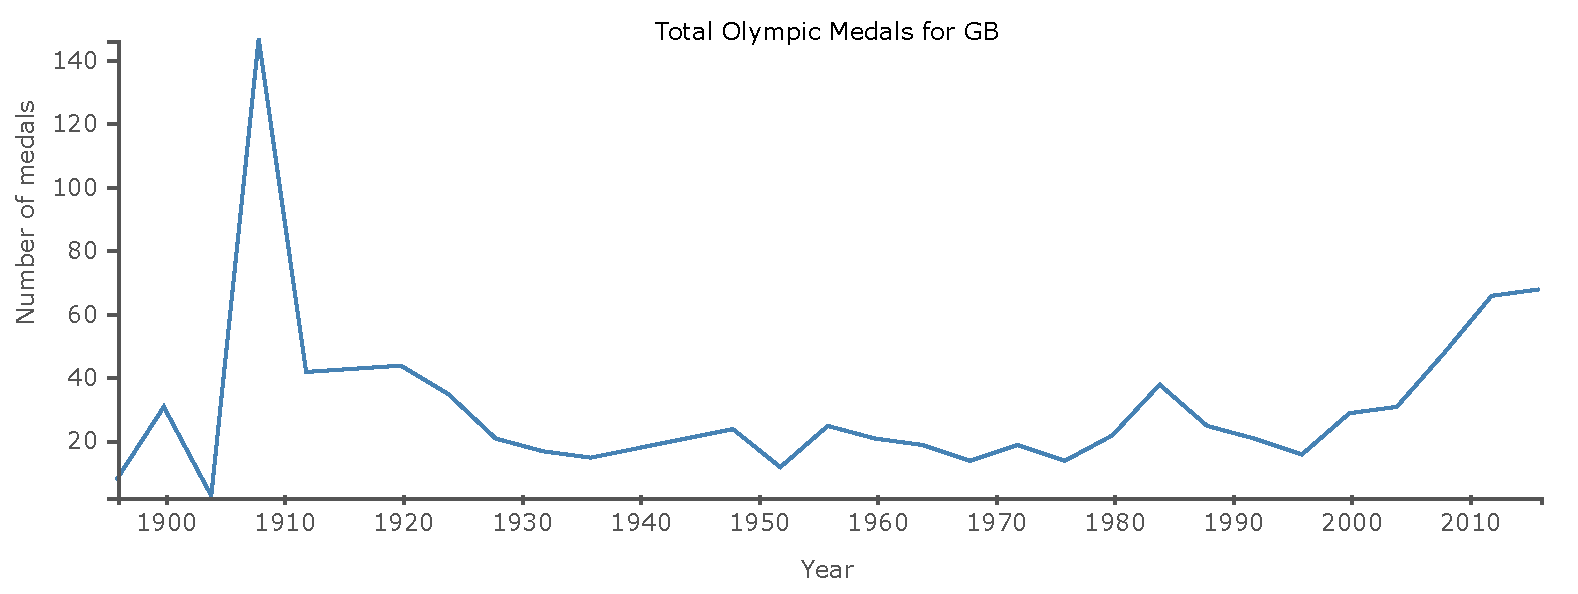
\includegraphics[width=65\resplinewidth]
{diagrams/resp-line-1.pdf}%
\label{fig:RespLineExample1}%
}
\hfill
\subfloat[][%
40rem
]
{%
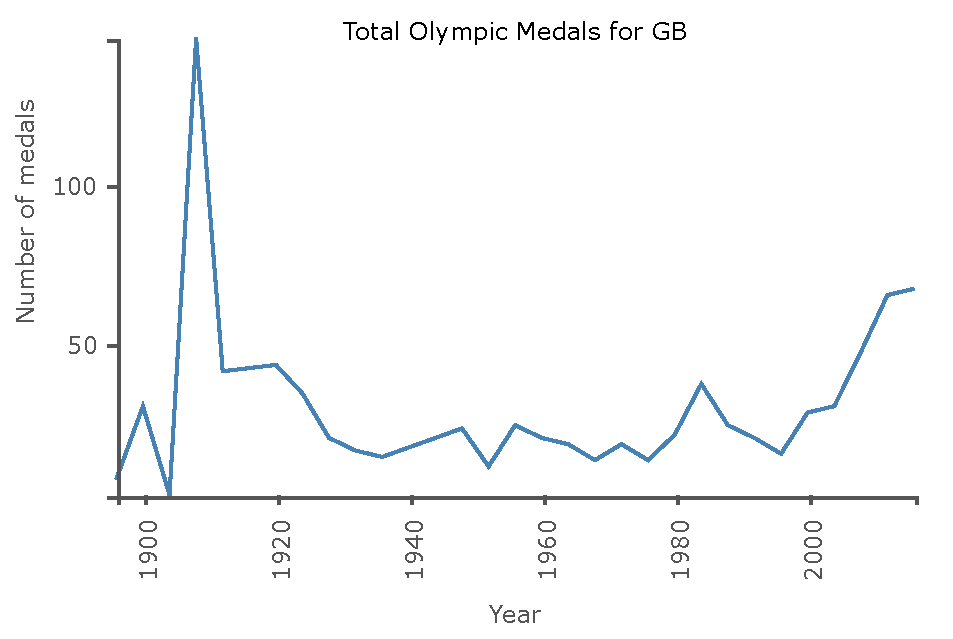
\includegraphics[width=40\resplinewidth]
{diagrams/resp-line-2.pdf}%
\label{fig:RespLineExample2}%
}
\hfill
\subfloat[][%
20rem
]
{%
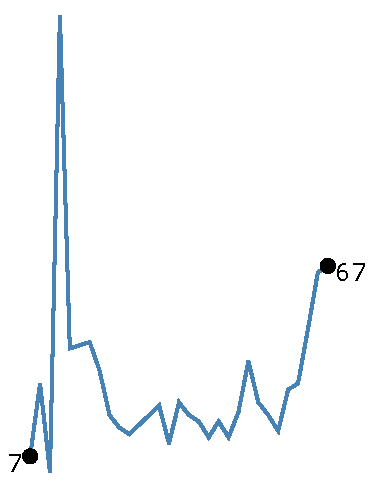
\includegraphics[width=20\resplinewidth]
{diagrams/resp-line-3.pdf}%
\label{fig:RespLineExample3}%
}
\caption[Responsive Line Chart Example]
{
A responsive line chart at different display widths.
\subref{fig:RespLineExample1} At 65rem, the x axis labels are
horizontal. \subref{fig:RespLineExample2} At 40rem, the x axis ticks
have been thinned out and the labels fully rotated by 90\textdegree.
\subref{fig:RespLineExample3} At 20rem, both axes have been removed,
and the chart has become a sparkline.
\imgcredit{Screenshots of \textcite{RespVisPage} created by the author of
  this thesis. Used with kind permission by Keith Andrews.}
}
\label{fig:RespLineExample}
\end{figure}









\subsection{Point Charts}
\label{sec:ScatterplotExamples}

Point charts, also known as scatterplots, represent data as points in
2d Cartesian coordinate systems. There are many examples of
point charts published as static images \parencite{Scatter,Scatter2},
with responsive versions starting to emerge. The first step to making
point charts responsive is to reduce their width to fit them into the
space available. As for other types of charts, care must be taken to
avoid overlapping of labels and annotations by applying recomposition,
relocation and simplification patterns
\parencite{RespScatter,RespScatter2}. To counteract the increased
density of points when reducing the size of their container, various
interaction features are usually implemented in point charts to aid
consumers in interpreting the represented data. The most useful
interaction features in these charts are elaborative zooming
interactions and the explorative panning interactions. In addition to
zooming and panning, \textcite{RespVis} employs additional methods to
ameliorate the overlapping of individual points, including fisheye
distortion, Cartesian distortion, and temporary displacements of
points.

An interesting technique for responsive point charts based on the
visualization's density (data points per pixel) rather than its width
was introduced by \textcite{NickRabinowitzRDV}. The benefit of this
approach is that charts adapt to changing amounts of data and
reconfigure their appearance accordingly. The patterns applied in the
responsive point chart shown in Figure~\ref{fig:RespScatterExample}
are the recomposition of annotations to only show annotations for
selected data records, and the switching of the encoding from a point
chart to a heatmap for high point densities. Other techniques, such as
the recomposition of data records, would also be applicable to
responsive point charts, but no examples for such patterns could be
found. If the data to be encoded is inherently cyclic, a radial point
chart, using polar coordinates, can be used to better reflect the
cyclic nature of the data \parencite{RespRadialScatterHLine}.



\begin{figure}[tp]
\centering
\subfloat[][%
Low density % (0.00005 points per pixel).
]
{%
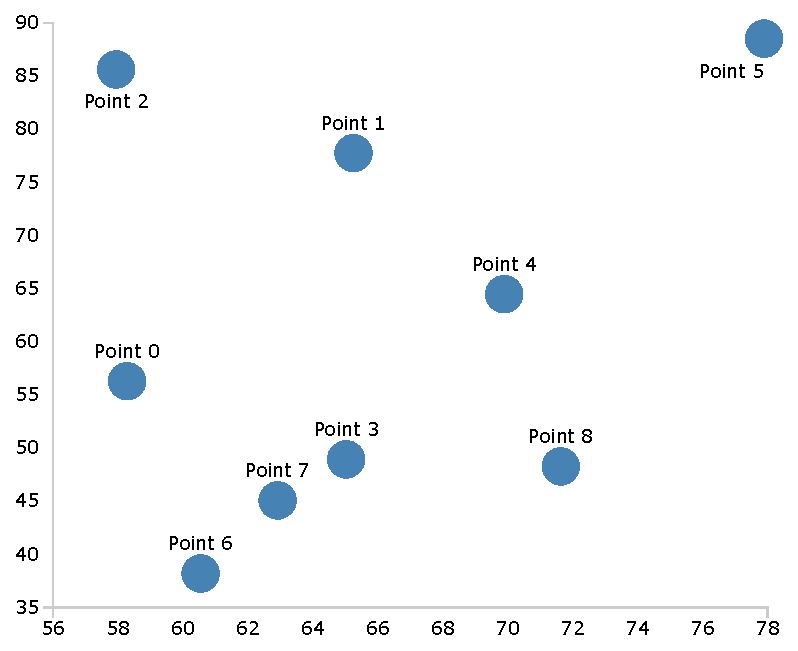
\includegraphics[width=0.3\linewidth]
{diagrams/resp-scatter-1.pdf}%
\label{fig:RespScatterExample1}%
}
\hfill
\subfloat[][%
Medium density % (0.0007 points per pixel).
]
{%
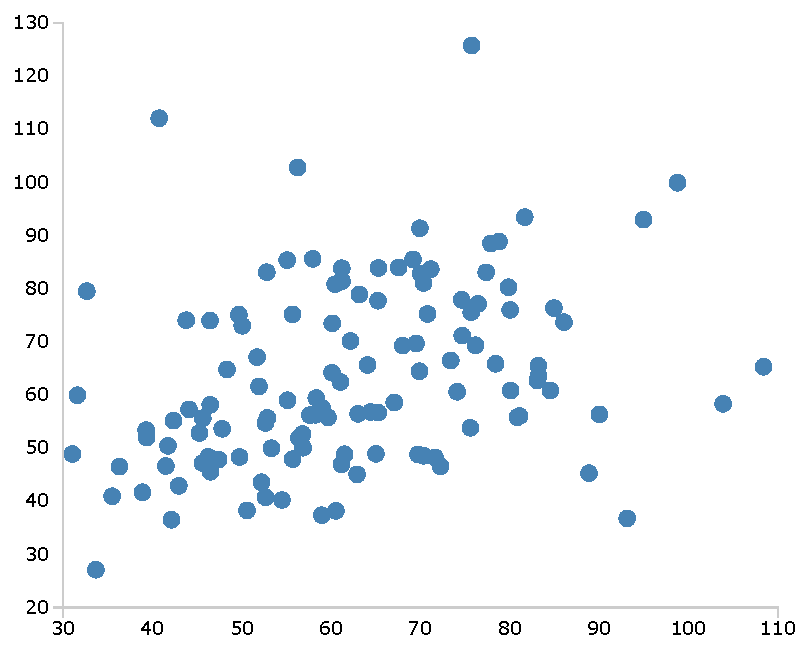
\includegraphics[width=0.3\linewidth]
{diagrams/resp-scatter-2.pdf}%
\label{fig:RespScatterExample2}%
}
\hfill
\subfloat[][%
High density % (0.017 points per pixel).
]
{%
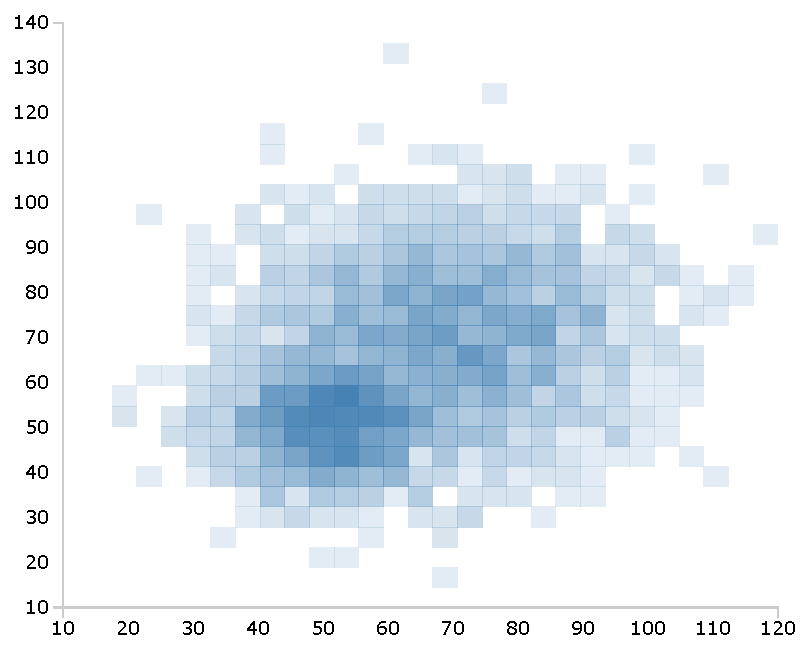
\includegraphics[width=0.3\linewidth]
{diagrams/resp-scatter-3.pdf}%
\label{fig:RespScatterExample3}%
}
\caption[Responsive Point Chart Example]
{
A responsive point chart based on data density (data
points per pixel). \subref{fig:RespScatterExample1} With a small
number of data points, all points and their corresponding labels are
shown. \subref{fig:RespScatterExample2} At a certain density, labels
are only shown for selected points. \subref{fig:RespScatterExample3}
At very high densities, the point chart is replaced by a heatmap to
more efficiently display the large amount of data.
\imgcredit{Screenshots created by the author of this thesis.
Visualization created by \textcite{NickRabinowitzRDV}}
}
\label{fig:RespScatterExample}
\end{figure}


\subsection{Parallel Coordinates}

Even though parallel coordinates charts
\parencite{ParallelCoordinates} are rarely encountered in
non-technical contexts, they are quite popular when it comes to
visualizing multidimensional data in visual analytics systems
\parencite{HighD}. In these kinds of charts, multiple dimensions are
rendered as parallel axes, upon which points are connected via paths
(polylines). Each polyline represents a data record and its values at
the corresponding dimensions. The axes of a parallel coordinates chart
are typically laid out horizontally, meaning that the chart can be
made narrower by reducing the distance between individual axes.
Previously mentioned axis-related responsive patterns, such as
rotating labels and recomposing ticks, can also be applied.

Another technique is to temporarily hide some dimensions, based on
some criteria. When automatically hiding dimensions, it is necessary
to apply compensation patterns, giving the visualization consumer
additional controls to configure which dimensions are displayed and
override the system's hiding behavior. An example of a responsive
parallel coordinates chart incorporating some of these patterns can be
seen in Figure~\ref{fig:RespParCoordExample}.
%
If reducing the chart's complexity is not appropriate, an alternative
is to transpose the chart, so its dimensions are laid out vertically
and vertical scrolling can be used to explore the full chart.




\begin{figure}[tp]
\newcommand{\respparcoordscale}{0.36}
\centering
\subfloat[][%
61rem
]
{%
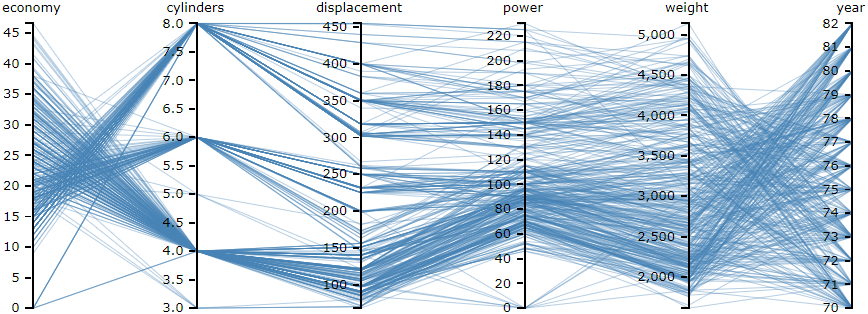
\includegraphics[valign=b,scale=\respparcoordscale]
{images/resp-parcoord-1.png}%
\label{fig:RespParCoordExample1}%
}
\hfill
\subfloat[][%
50rem
]
{%
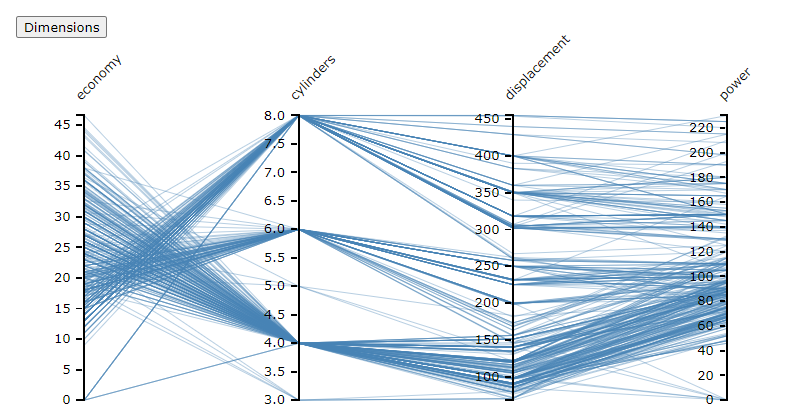
\includegraphics[valign=b,scale=\respparcoordscale]
{images/resp-parcoord-2.png}%
\label{fig:RespParCoordExample2}%
}
\newline
\subfloat[][%
40rem
]
{%
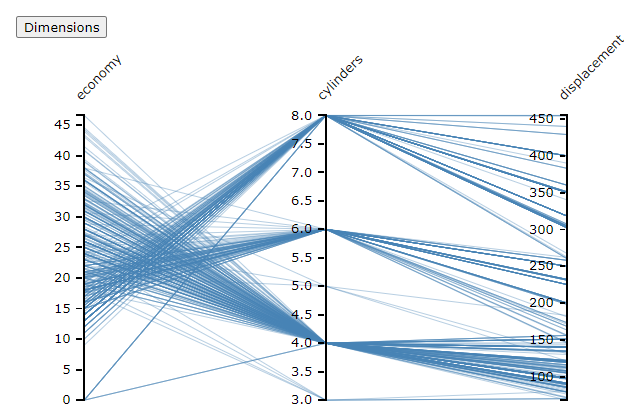
\includegraphics[valign=b,scale=\respparcoordscale]
{images/resp-parcoord-3.png}%
\label{fig:RespParCoordExample3}%
}
\hfill
\subfloat[][%
30rem
]
{%
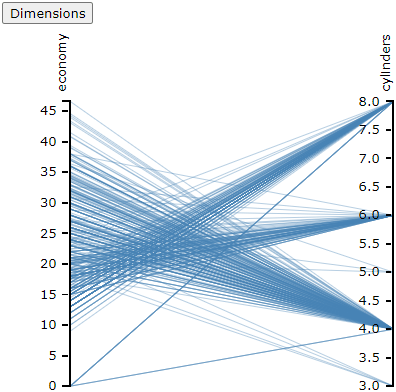
\includegraphics[valign=b,scale=\respparcoordscale]
{images/resp-parcoord-4.png}%
\label{fig:RespParCoordExample4}%
}
\hfill
\subfloat[][%
30rem, consumer-configured dimensions
]
{%
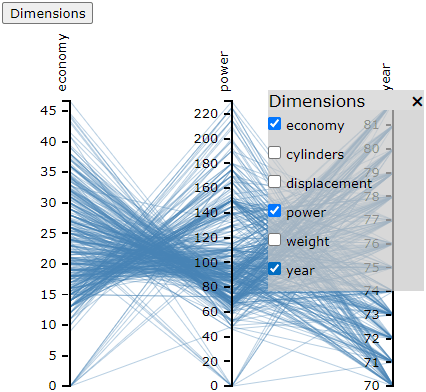
\includegraphics[valign=b,scale=\respparcoordscale]
{images/resp-parcoord-5.png}%
\label{fig:RespParCoordExample5}%
}
\caption[Responsive Parallel Coordinates Chart Example]
{ A responsive parallel coordinates chart at different display widths.
\subref{fig:RespParCoordExample1} At larger widths, all dimensions are
shown. \subref{fig:RespParCoordExample2} Dimensions are removed based
on their priority, dimension labels are rotated by 45 degrees, and a
dimensions toggle is shown which enables the configuration of
dimensions. \subref{fig:RespParCoordExample3} Further dimensions are
removed. \subref{fig:RespParCoordExample4} Further dimensions are
removed, and dimension labels are rotated by 90 degrees.
\subref{fig:RespParCoordExample5} The dimension configuration panel
has been opened, and the visualization consumer has taken control over
which dimensions to show. \imgcredit{Screenshots of
\textcite{RespVisPage} created by the author of this thesis. Used with
kind permission by Keith Andrews.} }
\label{fig:RespParCoordExample}
\end{figure}

       

\cleardoublepage

\chapter{The RespVis Library}
\label{chap:RespVis}

RespVis is an open-source D3 extension library for creating responsive
SVG charts \parencite{RespVisGitHub,RespVisLive}. It enables the use
of CSS for the responsive styling and layout of
visualizations. RespVis renders visualizations as pure and complete
SVG documents, meaning that the whole visualization is contained in
one SVG document and includes no elements of other XML namespaces.
RespVis is designed as an extension to D3, rather than a wrapper
around it. Unlike most other visualization libraries built on top of
D3, RespVis does not hide D3 behind a custom API. Rather,
visualization authors invoke RespVis functionality by binding
specially structured data to D3 Selections, which render visualization
components using render functions to transform the bound data into
some form of visual representation. Furthermore, RespVis espouses the
strong separation between data and code and applies strong static
type-checking through the use of TypeScript.






\section{Design}
\label{sec:Design}

The design of the RespVis library is guided by six principles:
\begin{enumerate}
\item Style and Layout via CSS.
\item Pure and Complete SVG Documents.
\item Extend D3.
\item Separate Data and Code.
\item Strong Static Type-Checking with TypeScript.
\item Layered Component Hierarchy.
\end{enumerate}




\subsection{Style and Layout via CSS}

Every part of a visualization that can be configured with CSS should
be configured with CSS. The visual appearance and layout of HTML
elements can already be configured by CSS. Many presentation
attributes of SVG elements can also be styled with CSS. However,
CSS-based layouting cannot be applied to SVG elements, which seriously
limits the responsive capabilities of using CSS for SVG charts.
Without powerful CSS layout technologies like Flexbox and Grid, all
the individual components of an SVG chart have to be positioned
manually via JavaScript.

The RespVis Layouter enables the layouting of visualization components
using powerful standard CSS-based layout mechanisms such as Flexbox
and Grid, by calculating the bounding boxes of SVG elements from the
CSS configuration of a shadow \elname{<div>} hierarchy. The Layouter
offers visualization authors comparable configurability to what they
are used to when laying out HTML elements. For example, a legend can
be configured to be placed to the right of a chart in a wider view,
and beneath the chart in a narrower view, using familiar CSS
constructs.





\subsection{Pure and Complete SVG Documents}

Every RespVis visualization should be rendered as a pure and complete
SVG document. An SVG document is considered \emph{pure}, if it
contains only elements defined in the SVG namespace. This means that
it must not contain any \elname{<foreignObject>} elements, which embed
elements of an XML namespace other than SVG, for example to embed HTML
elements inside an SVG. RespVis does not support rendering to HTML
canvas elements, because graphics rendered there cannot be styled by
CSS.

An SVG document representing a visualization is considered
\emph{complete}, if it contains the entire visualization within
it. Splitting visualization components across multiple SVG documents
is considered bad practice, because these components conceptually
belong together and should be represented as a whole. Having
a full visualization enclosed in a complete SVG document allows the
whole visualization to be exported and stored as a standard-compliant
SVG file, which can be further processed using a wide range of tools.




\subsection{Extend D3}

RespVis is designed as a library which extends D3, rather than a
wrapper around D3. Compared to other visualization libraries which
wrap a layer around D3, it does not provide an entirely new interface
to visualization authors, but uses D3 Selections as the core interface
with which to interact. The typical workflow of invoking RespVis
functionality is to bind data objects of a specific structure to the
elements of a Selection and then to visualize this data by calling a
render function to transform it into visual marks. If D3 were hidden
behind a custom API, its powerful capabilities would not be directly
accessible to users of the library, and would need to be exposed
manually through special mechanisms. By designing RespVis as an
extension of D3, visualization authors can continue to leverage its
expressive and concise API and author their documents using data joins
and the general update pattern.



\subsection{Separate Data and Code}

In RespVis, data and code are decoupled from each other. Everything in
RespVis is built from functions and objects without using any classes.
Classes were avoided, since they are not common when working with D3,
and also because they lead to a tight coupling between data and
functionality, which was deemed undesirable. The decoupling of data
and code results in various benefits compared to the prevalent
object-oriented way of building software. Among these benefits are
easier reuse and testing of functions and a software system which
requires less cognitive effort to understand.

Functions are easier to reuse because they only require well-shaped
input data to perform their task. Mechanisms like inheritance or
composition, which tend to increase the complexity of a system, are
unnecessary. Compared to class-based code, where an object needs to be
instantiated before testing its methods, it is easier to test
functions in isolation when they are not coupled to their data. The
reason for this is that the instantiation of an object might be a
complex operation dependent on other methods which could affect the
results of a test case.

Possibly the main benefit of decoupling data and code lies in the
reduced complexity of the resulting system. A software system which
treats data and code as different entities might be composed of more
entities than a system which does not, but the individual entities
have fewer dependencies between one another. The reduced number of
dependencies between entities results from separating entities into a
data entities group and a function entities group, with no
relationships between them. The research related to software
complexity is hard to convey in simple terms, but one rule of thumb is
well summarized by \textcite{DataCodeSeparation} as \enquote{A system
  made of disjoint simple parts is less complex than a system made of
  a single complex part.} Of course, there are also drawbacks when
designing a system adhering to this concept, but they are not too
severe and are therefore not listed here. For further reading on this
topic, the reader is directed to Moseley and Marks' classic workshop
paper \parencite{OutOfTarPit} and Sharvit's forthcoming book
\parencite{Sharvit-Book}.




\subsection{Strong Static Type-Checking with TypeScript}

The RespVis library is written in TypeScript, with everything being as
strongly-typed as possible. For the most part, interfaces are used to
describe the structure of data objects, and function parameters are
annotated with types. Whenever working with D3 Selections, their
contents are typed as strongly as possible using the generic type
variables available on Selections. Most of the time, it is sufficient
to specify only the type of elements contained in a Selection and the
structure of the data bound on them. If the element and data types of
a Selection are declared, the various functions can assume that
parameters passed to them have specific types, and they do not have to
worry about dynamic type checking. Applying a strongly typed system
has many advantages, such as better development tooling and
compile-time identification of type-related bugs. These advantages are
described in Section~\ref{sec:TS}.







\subsection{Layered Component Hierarchy}

Components in RespVis are structured in four layers with increasing
levels of abstraction, as shown in Figure~\ref{fig:Layers}. Components
in higher layers make more assumptions about their content than
components in lower layers. The bottom-most layer with the lowest
level of abstraction consists of visual Primitives, represented by
basic SVG elements like \elname{<rect>}, \elname{<circle>}, and
\elname{<text>}. These Primitives do not require any data to be bound to
them and are simply rendered by setting their attributes to the
desired values.


\begin{figure}[tp]
\centering
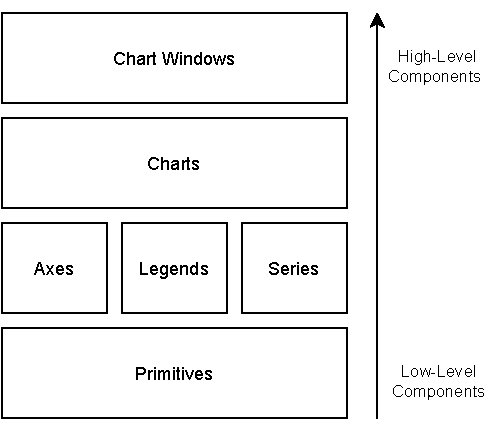
\includegraphics[keepaspectratio,width=\linewidth,height=7.5cm]
{diagrams/respvis-layers.pdf}
\caption[Component Layers of RespVis]{
The four layers of components in the RespVis library. Higher layers
contain increasingly higher-level components.
\imgcredit{Image created by the author of this thesis.}
}
\label{fig:Layers}
\end{figure}


The second layer comprises composite components such as Axes, Legends,
and Series. These are usually rendered as \elname{<svg>} or \elname{<g>}
elements containing only primitive elements. The components in this
layer are the lowest-level components which are configured using
structured data bound to their elements. Series components are
composite elements which render a collection of underlying elements
using a data join and the general update pattern.

The third layer consists of Chart components. Charts are composite
components which can also include other composite components. They are
the visual entities which represent complete visualizations and are
usually composed of axes, series, and legends.

In many other visualization libraries, charts are the highest-level
components visualization authors can work with, but RespVis contains
an additional layer above them, formed by Chart Window components.
Chart Windows are wrapper components around Charts. Unlike the
previously discussed lower layers, Chart Windows are not rendered as
SVG elements but as HTML \elname{<div>} elements. Their purpose is to
nest Charts into a Layouter component, render them in a three-phased
rendering process, and provide an optional toolbar for them. Toolbars
are customizable and can hold different tools for different types of
chart.








\section{Naming Conventions}
\label{sec:NamingConventions}

The naming of entities in RespVis follows the same naming conventions
used in D3 modules. The names of entities usually start with the name
of the group to which an entity belongs and are then further narrowed
down by successively adding more words until the exact entity is
accurately described. This convention is referred to as
\enquote{top-down naming} in this thesis. An example of the top-down
naming convention can be seen in the D3 Scale
\parencite{D3Scale} and D3 Axis \parencite{D3Axis} packages, in
which entities are called things like \code{scaleLinear},
\code{scaleOrdinal}, \code{axisBottom}, and \code{axisLeft} rather
than \code{linearScale}, \code{ordinalScale}, \code{bottomAxis}, and
\code{leftAxis}. Since this is the exact opposite of how these
entities would be called in natural English, using such names
can feel odd for the uninitiated. However, experience shows working
with APIs which follow such a naming convention is easier than with
those which do not, since users of such APIs can easily discover
specialized entities by inputting the general entity type and browsing
through code completion suggestions provided by their development
tools. Hence, entity names in RespVis also follow this convention.

The RespVis public interface is made up of types and functions. Types
are usually written as interfaces and represent the shape of an
object. Type names are written in \code{PascalCase}
\parencite{PascalCase} and adhere to the top-down naming
convention. They always start with the group a type belongs to, and
further words are appended to distinguish ever more specialized
types. The naming of types can best be demonstrated by the different
names given to interfaces describing data objects to configure
different kinds of Bar Charts. Data objects for the configuration of
Basic Bar Charts are described by the \code{ChartBar} interface, those
of Grouped Bar Charts are described by the \code{ChartBarGrouped}
interface, and those of Stacked Bar Charts are described by the
\code{ChartBarStacked} interface.

The API of RespVis is largely composed of functions. Function names
are always written in \code{camelCase} \parencite{camelCase} and also
follow the top-down naming convention. Function names always start
with the type of object on which they operate, followed by the
operation they perform. A component in RespVis always consists of a
data object which describes it, an element to which the data object is
bound, and a render function which transforms the bound data into some
form of visual representation. The names of functions to create data
objects for the configuration of components are always in the form of
\code{componentNameData}, such as \code{chartBarData} or
\code{chartBarGroupedData}. Functions which transform bound data into
a visual representation are always named in the form of
\code{componentNameRender}, such as \code{chartBarRender} or
\code{chartBarGroupedRender}.






\section{Project Structure}
\label{sec:ProjectSetup}

RespVis is a NodeJS \parencite{NodeJS} project hosted as an
open-source project on GitHub \parencite{RespVisGitHub}. It is
implemented in TypeScript and grouped into different packages by
thematic affinity. The TypeScript source files are compiled
(transpiled) to JavaScript and bundled into one combined library
package, which visualization authors can then import into their
projects.
%
The Rollup module bundler \parencite{Rollup} is used to perform
compilation and bundling. In addition to the bundled JavaScript
library, visualization authors are required to import an accompanying
CSS file containing default styling for the generated visualizations.
The project also contains examples demonstrating usage of the library
to create various charts. These examples are HTML files which import
the required files and contain JavaScript to invoke RespVis
functionality to create and update visualizations.
%
The Gulp \parencite{Gulp} task runner is used to automate the build
process of the library, including the preparation of the output
directory, the bundling of library code, and the copying of various
files to the correct locations in the output directory.




The RespVis project contains configuration files for various tools, a
\code{src/} directory containing the source code for the whole library
and accompanying examples, a \code{node_modules} directory containing
the project's cached NodeJS dependencies, and a \code{dist/} directory
containing built versions of the library and examples ready for
distribution. The configuration files are only discussed broadly here,
later sections go into more detail about the setup of the various
tools. An overview of the most important files and directories can be
seen in Figure~\ref{fig:RespVisDirTree}.

\begin{figure}[tp]
\centering
\framebox[\textwidth]{%
\begin{minipage}{0.9\textwidth}
\begin{footnotesize}
  \dirtree{%
  .1 /.
  .2 dist/.
  .3 examples/.
  .4 data/.
  .4 vendor/.
  .4 bar.html.
  .4 \dots.
  .3 index.html.
  .3 respvis.css.
  .3 respvis.[m]js.
  .3 respvis.[m]js.map.
  .3 respvis.min.[m]js.
  .3 respvis.min.[m]js.gz.
  .3 respvis.min.[m]js.map.
  .2 node\_modules.
  .2 src/.
  .3 lib/.
  .4 bars/.
  .4 core/.
  .4 legend/.
  .4 lines/.
  .4 points/.
  .4 tooltip/.
  .3 examples/.
  .4 data/.
  .4 vendor/.
  .4 bar.html.
  .4 \dots.
  .3 index.html.
  .3 respvis.css.
  .2 gulpfile.js.
  .2 package.json.
  .2 tsconfig.json.
  }
\end{footnotesize}
\end{minipage}
}
\caption[RespVis Directory Structure]{
  The most important files and directories of the RespVis project. 
  \imgcredit{Figure created by the author of this thesis.}
}
\label{fig:RespVisDirTree}
\end{figure}



The root directory of the RespVis project contains the necessary
project configuration files for NodeJS, TypeScript, and Gulp. The
NodeJS configuration file, \code{package.json}, describes the
meta-data of the NodeJS package. It is used to specify the project's
dependencies to other packages, and is required for every NodeJS
package, so that it can be uploaded to the npm package registry
\parencite{npm}. The TypeScript configuration file,
\code{tsconfig.json}, specifies the configuration the TypeScript
compiler uses to compile the library's TypeScript source files into
their JavaScript counterparts. The Gulp configuration file,
\code{gulpfile.js}, is used to describe atomic, recurring tasks and
compositions of them. These tasks can then be invoked via the Gulp
command-line tool to automate otherwise tedious workflow processes.

The \code{src/} directory at the root of the project contains all the
implementation files of the library in the \code{src/lib/} directory
and examples in the \code{src/examples/} directory. The
\code{src/lib/} directory contains all TypeScript source files of the
library. They are partitioned into packages formed around the thematic
affinity of the various components. The Core package
contains the core functionality of the library and is a prerequisite
for all the other packages. It includes the Layouter, Chart base
functionality, Chart Window base functionality, and various utility
functions. The Legend package contains modules to render
legends consisting of a title and configurable labeled symbols. The
Tooltip package contains functions to show and hide
tooltips, modify their contents, and position them. It also contains
helper functions for Series to prevent the replication of
tooltip-related code in their data creation and rendering functions.
The Bars, Lines, and Points packages
contain the necessary modules to render Series, Charts, and Chart
Windows for bar, grouped bar, stacked bar, line, and point
visualizations. At the moment, all these packages are built into a
combined one, but there are plans to also distribute them separately
to allow users of the library to import only the packages they need.

The \code{src/examples/} directory holds the source files of the
developed examples. These examples are distributed alongside the
library files, and are copied over to the \code{dist/examples/}
directory when building the project. Every example consists of an HTML
file which imports all the requirements such as \code{respvis.js} and
\code{respvis.css} as well as external dependencies such as D3. It
then invokes the necessary RespVis functionality within a
\elname{<script>} tag embedded in the body of the HTML document. In
addition to individual example files, the \code{examples} directory
also contains a \code{vendor} directory, which contains third-party
dependencies, and a \code{data} directory containing data imported by
individual examples.

In addition to configuration files and the \code{src/} directory, the
root directory also contains two directories which are automatically
generated during the build process. These are the \code{node_modules/}
and \code{dist/} directories. The \code{node_modules/} directory
exists in every NodeJS package. It is created when installing the
dependencies of a package and contains a cached copy of every
direct and indirect dependency. The \code{dist/} directory is
generated by the Gulp build tasks and contains all the files necessary
to distribute a built version of the RespVis library.

The code of the RespVis library is distributed as JavaScript bundles
in both the older IIFE (Immediately Invoked Function Expressions)
format and the more modern ES modules format. These formats are
explained in more detail in Section~\ref{sec:Rollup}. Bundles
containing the \code{.js} extension in their file name contain IIFE
source code, whereas bundles containing the \code{.mjs} extension
contain ES module source code. Furthermore, these bundles are also
distributed in minimized versions. The \code{dist/respvis.[m]js} file
contains the unmodified JavaScript bundle that can be used by library
consumers who require readable code, \code{dist/respvis.min.[m]js}
contains the minified JavaScript bundle, and
\code{dist/respvis.min.[m]js.gz} contains the minified JavaScript
bundle that has additionally been compressed in the GZIP format
\parencite{GZIP}. Alongside these code bundles, Rollup creates source
maps for the \code{dist/respvis.[m]js} and
\code{dist/respvis.min.[m]js} bundles: \code{dist/respvis.[m]js.map}
and \code{dist/respvis.min.[m]js.map}, respectively. These source maps
are interpreted by developer tools in browsers to map from certain
instructions in the bundled JavaScript code to the exact instruction
in the original TypeScript code and are immensely helpful for
debugging.


Since RespVis aims to perform all possible styling in CSS, the
distribution also contains a \code{dist/respvis.css} file with the
default styles for visualizations created with RespVis. Currently,
this file is written manually as a whole in the \code{src/} directory
and merely copied to the \code{dist/} directory during the build
process. In the future, this process could be improved by employing a
CSS preprocessing tool such as SASS \parencite{SASS}, so that the
styles can be split into multiple files during development. Besides
the bundled library source code and stylesheet, the \code{dist/}
directory also contains usage examples of RespVis in the
\code{dist/examples/} directory, copied over from the
\code{src/examples/} directory.






\section{NodeJS}

NodeJS is a standalone JavaScript runtime \parencite{NodeJS}, built on
top of the V8 JavaScript engine \parencite{V8}, which is an
open-source and multi-platform runtime for the execution of JavaScript
code. NodeJS allows JavaScript code to be run outside of web browsers.
NodeJS is heavily used for server-side development to unify the
technology stack of web developers and allow them to use JavaScript
for both client-side and server-side development. However, with the
appropriate project setup, NodeJS can be used for any kind of
development, and it can be set up as a powerful framework to develop
client-side applications as done in this project. One of the most
important tools in the NodeJS environment is the npm package manager
\parencite{npm}, which exists to simplify the sharing of packages and
their dependency management. The npm package registry hosts a huge
number of packages that can easily be imported and used to create new
ones.

RespVis is developed as an npm package. Every npm package is
configured via a \code{package.json} file. This file contains all the
necessary meta-data for a package to make it identifiable and provide
information about what the package contains. The \code{package.json}
file also lists all the dependencies of a package, so they can
automatically be updated and downloaded during an installation
process. A package can rely upon both normal dependencies and
development dependencies. Normal dependencies of a package are
required for it to work at run time and need to be installed alongside
it. Development dependencies are only required during development and
are only installed when installing a local package. The
\code{package.json} file is located in the root directory of the
RespVis package and can be seen in Listing~\ref{list:PackageJSON}.


\begin{samepage}
\lstinputlisting[%
  float=tp,
  aboveskip=\floatsep,
  belowskip=\floatsep,
  xleftmargin=0cm,              % no extra margins for floats
  xrightmargin=0cm,             % no extra margins for floats
  %
  basicstyle=\footnotesize\ttfamily,
  frame=shadowbox,
  numbers=left,
  label=list:PackageJSON,
  caption={[RespVis \code{package.json} File]%
    The \code{package.json} file of the RespVis library.
    This file contains all the meta-data describing the package and its dependencies.
    Keywords and type dependencies have been omitted for readability.
  },
]{listings/package.json}
\end{samepage}






\section{Rollup}
\label{sec:Rollup}

The Rollup module bundler \parencite{Rollup} is used to bundle the
source code of the RespVis library into bundles of different
kinds. Bundling combines code written as multiple smaller modules into
one combined package to make it easier to distribute. Developers do
not have to worry about the details of how their code will be
packaged, as Rollup takes care of all the necessary
transformations. In addition to bundling source code, Rollup also
performs \emph{tree shaking} on the bundled code, eliminating unused
code from the resulting bundle by statically analyzing dependencies
between modules.
%
Rollup supports the creation of bundles in several common module
formats, such as CommonJS, Asynchronous Module Definition (AMD),
Universal Module Definition (UMD), Immediately Invoked Function
Expressions (IIFE), and ES. RespVis is distributed as both IIFE and ES
modules.

IIFE modules have been used for a long time. They were used to support
modular software designs in JavaScript before more elaborate module
formats were defined. IIFE modules are anonymous functions which are
executed directly after declaring them. These functions contain the
full logic of the module and return an object representing its
publicly accessible interface. This object is usually stored in a
variable to allow interaction with the module after its creation.
IIFE modules are plain JavaScript and do not require any modern
features to be supported by browsers. They are simply loaded into web
documents like any other JavaScript resource via a \elname{<script>}
element. The example in Listing~\ref{list:IIFE} illustrates the IIFE
module format.



\begin{samepage}
\lstinputlisting[%
  float=tp,
  aboveskip=\floatsep,
  belowskip=\floatsep,
  xleftmargin=0cm,              % no extra margins for floats
  xrightmargin=0cm,             % no extra margins for floats
  %
  basicstyle=\footnotesize\ttfamily,
  frame=shadowbox,
  numbers=left,
  label=list:IIFE,
  caption={[IIFE Module Format]%
IIFE (Immediately Invoked Function Expression) modules wrap the module
code inside a function, which is executed immediately after declaring it
and returns the public interface of the module.
\code{do-something.js} contains the original code that should be
wrapped as an IIFE module, \code{module.js} contains the code of the
IIFE module, and \code{application.js} demonstrates usage of the
module.
},
]{listings/iife.js}
\end{samepage}



ES modules are a more recent addition to JavaScript, introduced in
ECMAScript 6 \parencite{ECMAScript6}. They are a native module system
built around the \code{import} and \code{export} statements, which are
widely supported by modern browsers. Since the individual modules of
the RespVis library are built as ES modules anyway, Rollup mostly only
has to merge them to create a valid, combined ES module. ES modules
are natively supported in browsers, so they can be loaded directly in
a HTML document using a \elname{<script>} element. However, it is
necessary to mark them as modules by setting the \attrname{type}
attribute to \code{module} on the loading \elname{<script>} element,
so that browsers can interpret them accordingly.


The core package of Rollup is only able to create mostly unmodified
bundles from JavaScript source files. Various plugins add
frequently required additional functionality. There are two kinds of
Rollup plugins: bundle plugins, which affect the bundling process, and
output plugins, which transform the already bundled code.

The Rollup bundle plugins used for the bundling of RespVis are
\code{@rollup/plugin-node-resolve}, \code{@rollup/plugin-commonjs},
and \code{@rollup/plugin-typescript}. The
\code{@rollup/plugin-node-resolve} plugin is used to resolve imports
from other NodeJS packages that reside in the \code{node_modules}
directory. Since many NodeJS packages are still implemented as
CommonJS modules, which are not natively supported by Rollup, the
\code{@rollup/plugin-commonjs} plugin is used to interpret them.
Lastly, the \code{@rollup/plugin-typescript} plugin is used to compile
TypeScript source files to JavaScript before bundling them. The
configuration for the TypeScript compiler is taken from the
\code{tsconfig.json} file at the root directory of the project.

The Rollup output plugins used during the bundling process are
\code{rollup-plugin-terser} and \code{rollup-plugin-gzip}. These
plugins do not affect every created bundle, but are used to
selectively transform the contents of specific bundles. The
\code{rollup-plugin-terser} plugin is used to create minified versions
of the RespVis bundles denoted by the term \code{.min} in their file
names. Logically, they are the same as the equivalent unminified
bundles, but are compressed as much as possible to reduce their file
size while still containing valid, but unreadable, JavaScript
code. The \code{rollup-plugin-gzip} plugin is used to create
compressed gzipped versions of the RespVis bundles denoted by the term
\code{.gz} in their file extensions \parencite{GZIP}.

Note that D3 is not included in any of the generated RespVis
bundles. RespVis is designed to be an extension of D3 and, most of the
time, an application wishing to use RespVis will already be using
D3. If D3 were to be included in the RespVis bundle, it would
unnecessarily be loaded a second time. To prevent D3 from being
included in the created bundles, all dependencies on D3-related
packages are marked as external.

The actual bundling is performed via the JavaScript API of Rollup in
the private \code{bundleJS} Gulp task. This task is executed in
various automation processes set up with Gulp, which are explained in
more detail in Section~\ref{sec:Gulp}. The code of the \code{bundleJS}
task can be seen in Listing~\ref{list:BundleJS}. The RespVis library
is bundled via the \code{Rollup.rollup} function which returns the
created bundle. This bundle is then written to one or more target
destinations via the \code{Bundle.write} method, which allows the
specification of the target bundle format and any plugins used to
transform the code before writing it.


\begin{samepage}
\lstinputlisting[%
  float=tp,
  aboveskip=\floatsep,
  belowskip=\floatsep,
  xleftmargin=0cm,              % no extra margins for floats
  xrightmargin=0cm,             % no extra margins for floats
  basicstyle=\footnotesize\ttfamily,
  frame=shadowbox,
  numbers=left,
  label=list:BundleJS,
  caption={[Gulp Task to Bundle RespVis]%
The private Gulp task which bundles the code of the RespVis libary.
The bundle is created once and then written to multiple targets.
}
]{listings/bundle-js.js}
\end{samepage}
  





\section{Gulp}
\label{sec:Gulp}

Gulp is a task runner which automates workflow processes via a set of
named tasks \parencite{Gulp}. It is used to automate processes like
building the library and serving examples on a development server.
Tasks are useful for automating operations which need to be carried
out repeatedly. They can perform an atomic operation or be composed of
other tasks. Composite tasks can execute tasks contained in them in
serial or in parallel. The tasks are implemented as JavaScript
functions in the Gulp configuration file, \code{gulpfile.js}, which
can be found in the root directory of the project. Gulp's approach of
favoring code over declarative configuration files means that the
person setting up process automation needs to be familiar with
JavaScript. In return, the possibilities for configuration are
endless.

Tasks in the \code{gulpfile.js} file are separated into private and
public tasks. Private tasks are simply asynchronous functions which
perform a certain action that does not necessarily have to be executed
by external entities. The private tasks in the RespVis project are
\code{bundleJS}, \code{bundleCSS}, \code{copyExamples},
\code{cleanDist}, \code{cleanNodeModules}, and \code{reloadBrowser}.
%
Public tasks are also asynchronous functions, but they are exported
and are therefore available to be executed via the Gulp command-line
interface. Most public tasks in the RespVis project are compositions
of other tasks. The public tasks in RespVis are \code{clean},
\code{cleanAll}, \code{build}, and \code{serve}. The default task,
\code{serve}, is executed when no other task is specified on the
command line. A hierarchical representation of all the tasks in the
\code{gulpfile.js} file is shown in Listing~\ref{list:GulpTasks}.

\begin{samepage}
\lstinputlisting[%
  float=tp,
  aboveskip=\floatsep,
  belowskip=\floatsep,
  xleftmargin=0cm,              % no extra margins for floats
  xrightmargin=0cm,             % no extra margins for floats
  %
  basicstyle=\footnotesize\ttfamily,
  frame=shadowbox,
  numbers=left,
  label=list:GulpTasks,
  caption={[Tasks Defined in \code{gulpfile.js}]%
A hierarchical representation of the tasks defined in the \code{gulpfile.js} file,
as output by the \code{gulp --tasks} command.
},
]{listings/gulp-tasks.txt}
\end{samepage}
  


Bundling the RespVis library's source code is implemented in the
private \code{bundleJS} task. It uses the JavaScript API of Rollup to
compile the TypeScript source files into JavaScript and bundle them
into IIFE and ES modules of varying levels of minification. This task
has already been described in detail in Section~\ref{sec:Rollup}, so
it won't be discussed further here. It is executed during the public
\code{build} and \code{serve} tasks.

The \code{bundleCSS} task is used to copy the \code{src/respvis.css}
file to the \code{dist/} directory. Since one of the design pillars of
RespVis is to style everything possible with CSS, this file contains
all the default styles for visualizations created with
RespVis. Currently, this file is one large single file in the
\code{src/} directory and is merely copied over to the \code{dist/}
directory, but there are plans to build this file from different
modules using a CSS preprocessor in the future, which will require an
additional bundling step. This task is executed as part of the public
\code{build} and \code{serve} tasks.

The private \code{copyExamples} task copies all the files from the
\code{src/examples/} directory to the \code{dist/} directory. This
task is required because the examples are developed inside the
\code{src/} directory, but need to be made available in the
distributable library packages. Another reason for the copying is that
the BrowserSync development server is initialized with the
\code{dist/} directory as its root, and every potentially viewable
file must reside somewhere in that directory. The \code{copyExamples}
task is executed during the public \code{build} and \code{serve}
tasks.

The private \code{cleanDist} and \code{cleanNodeModules} tasks are
used to delete the \code{dist/} and \code{node_modules/} directories,
respectively. The \code{cleanDist} task is additionally exported as
the public \code{clean} task. This task is necessary because without
cleaning the \code{dist/} directory before every rebuild, redundant
files from previous builds that might have disappeared in the meantime
would cause littering and confusion. Therefore, this task is executed
as the first step of the \code{build} task. The public \code{cleanAll}
task is composed of the private \code{cleanDist} and
\code{cleanNodeModules} tasks. It is manually executed by a developer
to delete the currently cached dependencies of the project, to then
reinstall them from scratch.

The public \code{build} task is responsible for building all parts of
the project. It is a composite task which executes the \code{clean},
\code{bundleJS}, \code{bundleCSS}, and \code{copyExamples} tasks. The
\code{clean} task is invoked before all of the other tasks, which are
then executed in parallel. After this task finishes, the \code{dir/}
directory will contain all distributable JavaScript and CSS files of
the library, as well as the distributable \code{examples/} directory.

To simplify the development of RespVis, a Browsersync
\parencite{Browsersync} development server is used to host the built
distributables. Browsersync is a useful tool for synchronized browser
testing during development. It has many features like simulated
network throttling, interaction synchronization, and file
synchronization, which enable simultaneous testing in multiple
environments. For RespVis, it is only used for its ability to
synchronize and hot-reload files on the fly. The public \code{serve}
task, which is also exported as the default task, initializes a
Browsersync development server which serves files from the
\code{dist/} directory. Automatic reloading of the development server
is implemented manually via the \code{Gulp.watch} function. This
function enables a task to be executed whenever a change to a watched
file (matched by the supplied glob pattern) is detected. The
\code{serve} task implements three different cases which cause the
development server to reload. Firstly, every time one of the
TypeScript files in the \code{src/lib/} directory changes, the
\code{bundleJS} task is executed, and the browser is
reloaded. Secondly, every time the \code{src/respvis.css} file
changes, the \code{bundleCSS} task is executed, and the browser is
reloaded. Thirdly, whenever a file in the \code{src/examples/}
directory is changed, the \code{copyExamples} task is executed, and
the browser is reloaded.


     

\cleardoublepage
\chapter{Modules}
\label{chap:Modules}

The source code of RespVis is structured into modules written in the ES module format.
Currently, all individual modules are combined into a single, monolithic library bundle during the build process, but this will be changed in the future so that users can import only the modules they need.
The reason for this is that most users will likely only require a subset of all the features included in the library, and it would unnecessarily increase the size of their bundles to import all of them.
A good example of this is D3, which also separates its considerable amount of features into different modules that can be successively added to a project when the need arises.

At the time of writing, the RespVis library contains the Core, Legend, Tooltip, Bar, and Point Modules with each of them containing various submodules that have been grouped by thematic similarity.
The Core Module holds the core functionality of the library that all other modules depend on and includes the Layouter and Axis Components, Chart and Chart Window base functionality, and various utility functions and types.
The Legend Module contains the implementation of a Legend Component that is mostly meant to describe discrete data by rendering distinct values as labeled symbols.
The Tooltip Module holds functions to control the showing, placement, and content of Tooltips, as well as utility functions that simplify the configuration and initialization of Tooltips on Series Components.
The Bar Module distinguishes between Single-Series, Grouped, and Stacked Bars and includes various low-level and high-level components to render each of those types.
Similarly, the Point Module contains low-level and high-level components to visualize Point Charts.
All of the different modules and the dependencies between them are shown in Figure~\ref{fig:Modules}.

\begin{figure}[tp]
\centering
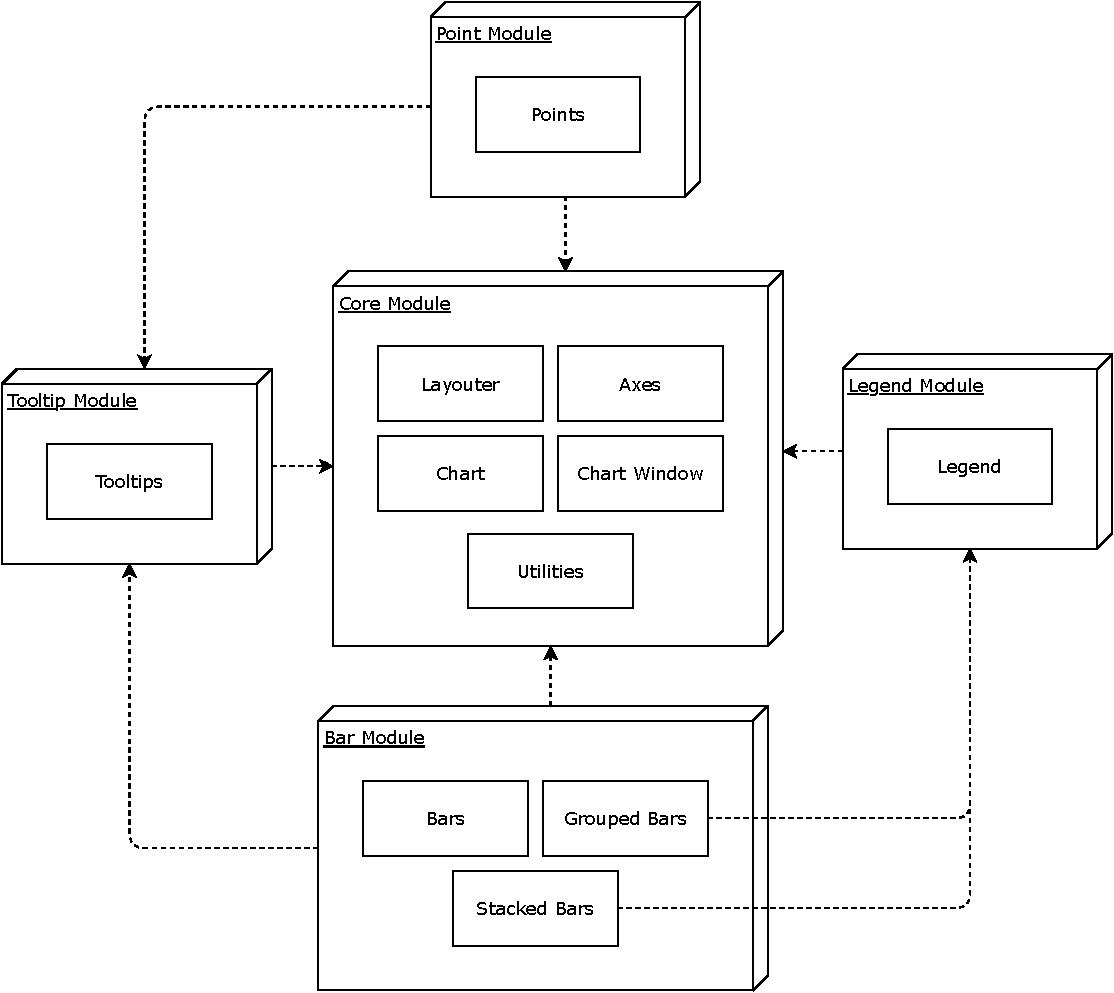
\includegraphics[keepaspectratio,width=\linewidth,height=\fullh]{diagrams/respvis-modules.pdf}
\caption[Modules of RespVis]{
  This diagram shows the different modules of the RespVis library.
  It also shows the most important submodules contained in the individual modules.
  The directional arrows connecting modules indicate dependencies between them.
  \imgcredit{Image created by the author of this thesis using \href{https://www.diagrams.net/}{diagrams.net}.}
}
\label{fig:Modules}
\end{figure}


\section{Core Module}

The implementation of the Core Module is located in the \code{src/lib/core/} directory of the project and contains the necessary core functionality of the library that forms the base on which all other modules depend.
It includes various utility functions, the Layouter, Axes, Chart base functionality, and Chart Window base functionality.
RespVis heavily relies on utility functions to reuse recurring operations, and the Core Module contains utilities that simplify the handling of arrays, elements, Selections, texts, positions, sizes, rectangles, circles, and paths.
The Layouter is a custom component that enables controlling the layout of SVG elements with CSS.
Axis Components have been included in the Core Module because they are important components that occur in nearly all visualizations.
Lastly, the Core Module offers base functionalities for Charts and Chart Windows that simplify the creation of more specialized Chart and Chart Window Components.

\subsection{Utilities}

The utilities provided by RespVis are split into multiple submodules that are placed in the \code{utilities/} directory of the Core Module.
These modules include types and functions that perform array, element, Selection, and text operations, as well as modules that simplify geometric operations with positions, sizes, rectangles, circles, and paths.
Utility functions are grouped into submodules by the type of entity on which they operate, which is is also reflected in the utility function names.
The names of utility functions follow the top-down naming convention described in Section~\ref{sec:NamingConvention}, which means that the names all begin with the type of entity with which the function is associated.

Array utilities can be found in the \code{utilities/array.ts} module.
The \code{Array} class in the JavaScript base implementation already offers a wide variety of convenient methods to work with arrays.
These methods form a solid foundation to handle a broad range of situations, but not everything is covered, and some things require manual implementations, which is why the RespVis library offers additional functions that simplify commonly encountered tasks.
The \code{arrayEquals} function is used to verify the equality of two arrays and also works with arbitrary levels of nesting. 
Array type guard functions are used to determine at runtime whether or not a variable is an array, and the Array Utility Module provides two different ones: \code{arrayIs}, which evaluates to true if the passed parameter is any kind of array, and \code{arrayIs2D}, which evaluates to true if the handed parameter is a two-dimensional array.
The \code{arrayIs} function is merely an alias for the \code{Array.isArray} method and has been added to provide a consistent counterpart to the \code{arrayIs2D} type guard function.
The last function in the array utility module is the \code{arrayPartition} function, which receives an array and a partition size as parameters and returns a partitioned version of the input array with each chunk containing the number of items specified by the partition size parameter.


The Element Utility Module located at \code{utilities/elements.ts} in the Core Module contains functions and constants related to elements in a document.
The \code{elementRelativeBounds} function is used to calculate the bounding box of an element relative to the bounding box of its parent in viewport coordinates.
Internally, it uses the \code{getBoundingClientRect} function, which returns the actual bounding box of an element in viewport coordinates and, as opposed to other ways of accessing this information, this function also takes transformations into account.
Every element has a set of CSS styles applied to them, and the \code{Window.getComputedStyle} method can be used to query the active styles of elements.
The style declaration object returned by this method contains all possible CSS properties and their values, regardless of whether or not they are set to default values.
Sometimes this behavior may be desired, but in this library, the computed style is mainly used for the preparation of a downloadable SVG document to transform styling information set in CSS to attributes on the individual elements.
If every possible CSS property on every element would be mapped to an attribute, the resulting SVG document would be unnecessarily bloated and hard-to-read because only those properties that are not set to their default values actually have an effect.
For this reason, the \code{elementComputedStyleWithoutDefaults} function has been implemented to calculate the computed style of an element and remove all default-valued properties from the returned style declaration object.
This is implemented by adding a \code{<style-dummy>} element as a sibling of the element of interest, getting the computed styles of both elements, and calculating the difference between them.
To accelerate these calculations, the \code{elementComputedStyleWithoutDefaults} function accepts an array of property names as its second parameter and will only consider the properties listed in this array.
The constant \code{elementSVGPresentationAttrs} array contains the names of all SVG presentation attributes listed in the SVG 1.1 specification \parencite{SVG11}.
As soon as support for SVG 2 \parencite{SVG2} by most major browsers has reached maturity, this array will be extended to include any newly added presentation attributes. 
Since only these SVG attributes can be styled via CSS, only CSS properties representing presentation attributes have to be considered when preparing downloadable SVG documents.

Selection utilities are implemented in the \code{utilities/selection.ts} module and include typing improvements for the D3 \code{Selection}, \code{Transition}, and \code{SelectionOrTransition} interfaces and type guards to distinguish between them.
The \code{Selection}, \code{Transition}, and \code{SelectionOrTransition} interfaces allow the specification of four type variables: the type of elements contained in the Selection or Transition, the type of data bound to those elements, the type of the parents of those elements, and the type of data bound to those parents.
In most cases, the type variables related to parent elements do not influence the logic of code using these interfaces and could be omitted to keep it more concise.
For this reason, these interfaces have been reexported with default types set on all of the type variables, which means that whenever type variables need to be manually specified, only those that need to be set to specific types need to be explicitly stated.
Further typing improvements have been made to the \code{attr} and \code{dispatch} methods of the \code{Selection} interface.
The D3 type declarations of the \code{Selection.attr} method do not include \code{null} as a possible return value, which is wrong because this method will result in a \code{null} value when reading an attribute that does not exist.
To fix this inconsistency and catch potential bugs related to it during compilation, the type declaration of the \code{Selection.attr} method has been overwritten in the Selection Utility Module to include \code{null} as a possible return value.
A less important but convenient improvement has been made to the type declaration of the \code{Selection.dispatch} method, which allows the dispatching of custom events with certain parameters that control different aspects of how this event is dispatched and the data bound to it.
In practice, not all parameters need to be specified at every invocation because the implementation of the \code{Selection.dispatch} method will provide default values for all of them, but this is not reflected in the type declaration of the function, which requires every parameter to be set every time the function is called.
To fix this, the Selection Utility Module provides a type declaration overwrite for the \code{Selection.dispatch} function that wraps the type of the parameters parameter into the \code{Partial} utility type.
Apart from these typing improvements, this module also provides the \code{isSelection} and \code{isTransition} type guard functions that are used to distiguish between Selections and Transitions.


Utilities for dealing with \code{<text>} elements can be found in the \code{utilities/text.ts} module, which contains rather basic functionalities that simply set specific \code{data-*} attributes to specific values on \code{<text>} elements.
The Text Utility Module holds functions that set \code{data-*} attributes controlling the horizontal and vertical alignment of \code{<text>} elements, as well as their orientation.
Horizontal and vertical alignment is configured using the \code{textAlignHorizontal} and \code{textAlignVertical} functions, which respectively set the \code{data-align-h} and \code{data-align-v} attribute on \code{<text>} elements to the value passed into either function as a string enum parameter of type \code{HorizontalAlignment} or \code{VerticalAlignment}.
The \code{HorizontalAlignment} enum represents the string values \code{\"left\"}, \code{\"center\"} and \code{\"right\"}, while the \code{VerticalAlignment} enum represents the values \code{\"top\"}, \code{\"center\"} and \code{\"bottom\"}.
The distinct \code{data-align-h} and \code{data-align-v} attribute values are then used in Selectors of various CSS rules to declare different values for the \code{text-anchor} and \code{dominant-baseline} properties.
Text orientation is set using the \code{textOrientation} function, which sets the \code{data-orientation} attribute on \code{<text>} elements to the value specified via the \code{Orientation} string enum parameter.
The \code{Orientation} enum represents the values \code{\"horizontal\"} and \code{\"vertical\"}.
These \code{data-orientation} attribute values are then used in CSS to set the \code{text-anchor}, \code{dominant-baseline}, and \code{transform} properties of \code{<text>} elements, in order to rotate them accordingly and position them correctly inside their bounding box calculated by the Layouter.


The Core Module also contains utilities that simplify geometric operations.
One of these utility modules is the Position Utility Module located in the \code{utilities/position.ts} file, which contains the \code{Position} interface and various functions to perform operations related to it.
The \code{Position} interface consists of the \code{x} and \code{y} number properties.
Rounding these properties is necessary to be able to correctly compare the equality of two \code{Position} objects and to not render unnecessarily long strings when transforming them into string representations.
This rounding is performed with the \code{positionRound} function, which allows the specification of the number of decimals the properties should be rounded on.
Equality comparision between two \code{Position} objects can be done with the \code{positionEquals} function, which evaluates to \code{true} if all properties of both \code{Position} objects are equal and \code{false} if not.
The \code{positionToString} function can be used to transform a \code{Position} object into its \code{\"x, y\"} string representation, and its counterpart, the \code{positionFromString} function, can be used to transform a correctly-formatted string into a \code{Position} object.
A large part of RespVis consists of modifying the attributes of elements.
Therefore, the \code{positionToAttrs} function can be used to set the \code{x} and \code{y} attributes of elements to the values of the \code{x} and \code{y} members of a \code{Position} object, and similarly, the \code{positionToTransformAttr} function can be used to set the \code{transform} attribute of elements to a translation representing a \code{Position} object.
The Position Utility Module also contains the \code{positionFromAttrs} function, which can be used to create a \code{Position} object from an element's \code{x} and \code{y} attributes.

The Size Utility Module located in the \code{utilities/size.ts} file in the Core Module is very similar to the Position Utility Module.
It contains the \code{Size} interface, which consists of the \code{width} and \code{height} number properties, the \code{sizeRound} function to round the properties of a \code{Size} object to a certain number of decimals, and the \code{sizeEquals} function to compare two \code{Size} objects for equality.
Similar to the equivalent functions in the Position Utility Module, the \code{sizeToString} and \code{sizeFromString} functions can be used to convert between \code{Size} objects and their string representations, and the \code{sizeToAttrs} and \code{sizeFromAttrs} functions can be used to convert between \code{Size} objects and \code{width} and \code{height} attributes of elements.

Utilities for dealing with rectangles can be found in the Rectangle Utility Module, which is located in the \code{utilities/rect.ts} file of the Core Module.
This module contains the \code{Rect} interface, which is the union of the \code{Position} and \code{Size} interfaces and therefore describes an object with the \code{x}, \code{y}, \code{width}, and \code{height} number properties.
Similar to the Position and Size Utility Modules, this module contains the \code{rectRound} function to round \code{Rect} objects, the \code{rectEquals} function to compare two of them for equality, the \code{rectToString} and \code{rectFromString} functions to convert between \code{Rect} objects and their string representations, and the \code{rectToAttrs} and \code{rectFromAttrs} functions to convert between objects and \code{x}, \code{y}, \code{width}, and \code{height} attributes of elements.
Since the \code{Rect} interface is a combination of the \code{Position} and \code{Size} interfaces, most of the functions in this module internally use the functions provided by the Position and Size Utility Modules.
The \code{rectMinimized} function creates a minimized version of the passed \code{Rect} object, which is infinitely small and positioned at the original \code{Rect} object's center.
Minimized rectangles are used in transitions that grow or shrink \code{<rect>} elements from or to their centers. 
When declaring a stroke for SVG elements, it is drawn exactly on the outline of an element's shape, which means that a stroke will extend outside the original bounds of an element by half the stroke width.
This can lead to unwanted artifacts like the stroke of bars in a Bar Chart overlapping over the Chart's Axes.
To counteract this, the \code{rectFitStroke} function is offered by the Rect Utility Module to adjust the properties of \code{Rect} objects to account for a specific stroke width around them.
Lastly, the Rectangle Utility Module provides functions to calculate specific positions inside rectangles.
The most generic of these functions is the \code{rectPosition} function, which enables the calculation of a position inside a rectangle via a two-dimensional parameter that expresses a position as the percental width and height distance from a rectangle's top-left corner.
All other position-calculating rectangle utility functions are simply shorthand functions that internally call the \code{rectPosition} function.
The \code{rectCenter} function returns a \code{Position} object representing the center position of a \code{Rect} object.
The \code{rectLeft}, \code{rectRight}, \code{rectTop}, and \code{rectBottom} functions return \code{Position} objects that represent  the middle position of the corresponding edge of a \code{Rect} object.
Similarly, The \code{rectTopLeft}, \code{rectTopRight}, \code{rectBottomRight}, \code{rectBottomLeft} functions can be used to calculate the corner positions of a rectangle.

The last geometric primitives whose handling is simplified by a RespVis utility module are circles.
The Circle Utility Module can be found in the \code{utilities/circle.ts} file in the Core Module.
It contains the \code{Circle} interface, which describes a circle object via a \code{center} \code{Position} property and a \code{radius} number property.
This module also contains equivalent functions to those found in previously-mentioned utility modules: \code{circleRound}, \code{circleEquals}, \code{circleToString}, \code{circleFromString}, \code{circleToAttrs}, \code{circleFromAttrs}, \code{circleMinimized}, and \code{circleFitStroke}.
Furthermore, the \code{circlePosition} function can be used to calculate positions inside a circle using an angle that defines an offset direction and an offset distance from a circle's center as a percentage of the circle's radius.
The Circle Utility Module also contains functions to create circles from rectangles, which are the \code{circleInsideRect} function to calculate the largest circle that can fit inside of a rectangle and the \code{circleOutsideRect} function to calculate the smallest circle that encloses a rectangle.

The Path Utility Module is located in the \code{utilities/path.ts} file in the Core Module and provides functions that simplify the creation of path definitions that can be set as \code{d} attributes on \code{<path>} elements.
The \code{pathRect} function uses a \code{Rect} object to create a rectangle path definition that can be set on \code{<path>} elements instead of using \code{<rect>} elements.
Similarly, the \code{pathCircle} function uses a \code{Circle} element to create a circle path definition that can be set on \code{<path>} elements instead of using a \code{<circle>} elements.
The reasons for using \code{<path>} elements rather than more descriptive shape elements is that their shapes can be changed dynamically and that it is possible to smoothly transition between shapes by interpolating their path definition strings.

\subsection{Layouter}
\label{sec:Layouter}

The Layouter is the most novel contribution of this work.
It is a component that wraps around an SVG document and allows configuration of the layout of elements in this document with CSS.
Instead of implementing a custom layout algorithm, the Layouter builds on layout engines integrated into browsers, which have already been summarized in Section~\ref{sec:BrowserEngines}.
Earlier proof of concept implementations used the FaberJS \parencite{FaberJS} and Yoga \parencite{Yoga} layout engines to compute layouts, but these implementations were not further pursued because they limited layouting to either Grid or Flexbox-based constraints.
Furthermore, the use of already existing browser functionality in the current implementation leads to a reduced bundle size and to visualization authors being able to use all the layouting capabilities natively offered by browsers.

CSS has always been the foundation of responsive web design for HTML-based websites because of its ability to adapt an element's presentation and the possibility of defining different presentations for different contexts via media queries.
A large part of the responsive power that CSS offers comes from its ability to change the positioning and layout of elements.
As already mentioned in previous chapters, CSS can style certain aspects of SVG documents, but it is not possible to use CSS layouting techniques to position SVG elements.
Even though there are already other visualization libraries such as Chartist \parencite{Chartist} and Highcharts \parencite{Highcharts} that allow the use of CSS to style visualizations, none of them offer the possibility to modify the layout of visualizations via CSS, which means that visualization authors have to learn and use custom APIs to position elements, limiting the range of possible layouts to those supported by the individual libraries. 

The Layouter distinguishes between laid-out and non-laid-out elements because not every element in a visualization profits from being laid out.
The positions and sizes of laid-out elements are being calculated by the Layouter, whereas non-laid-out elements are ignored during the layout process.
Theoretically, the Layouter could be used to position all visualization elements since all that is necessary is to determine a good mapping for each element that maps the rectangular bounding box calculated by the Layouter to the desired SVG shape of the element.
However, the positioning of elements in a visualization is constrained more strictly than element positioning in typical HTML documents because the content of a visualization is communicated through visual features such as position, size, shape, and poximity of elements rather than simply through text which can be positioned much more freely.  
For this reason, many elements of a visualization must be positioned at specific locations with specific dimensions, which means there is very little profit in laying them out with an elaborate layout algorithm.
Instead, exactly-positioned elements like the \code{<rect>} elements of Bar Series and the \code{<circle>} elements of Point Series are usually positioned directly via their SVG attributes, as laying them out via the Layouter would be pointless and only cause unnecessary overhead.

The Layouter Module can be found in the \code{layouter.ts} file of the Core Module.
The main function that this module provides is the \code{layouterCompute} function which implements the three-phased layout process that can be seen in Figure~\ref{fig:LayoutProcess}.
These three phases are:
\begin{enumerate}
\item Replication:
The structure of the SVG document that shall be laid out must be replicated with HTML \code{<div>} elements because only HTML elements can be affected by CSS-based positioning.
These elements are referred to as \enquote{layout elements} and have the same classes and \code{data-*} attributes as the SVG elements they are replicating.

\item Layout:
The replicated layout elements are affected by CSS rules that configure their positioning and are automatically laid out by browsers. 
If the Selectors of CSS rules used to style SVG elements only select them using classes and \code{data-*} attributes, the layout of these elements can be directly configured in these rules because corresponding layout elements have the same classes and \code{data-*} attributes and these CSS rules will also be applied to them.

\item Synchronization:
In this phase, the positions of layout elements are synchronized with their respective SVG elements.
The calculated bounding boxes of layout elements are set as \code{bounds} attributes on SVG elements to make the boundary information available in subsequent renderings for the positioning of nested elements.
In addition to that, the Layouter sets different default attributes on different types of SVG elements that aim to represent the boundaries of individual elements.
\end{enumerate}

\begin{figure}[tp]
\centering
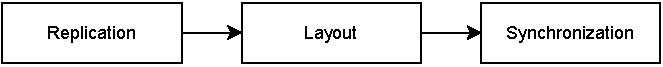
\includegraphics[keepaspectratio,width=\linewidth,height=\fullh]{diagrams/respvis-layout-process.pdf}
\caption[Layout Process of the Layouter]{
  This diagram shows the three phases of the layout process of the RespVis Layouter. 
  During the replication phase, the SVG document that shall be laid out is replicated with HTML \code{<div>} elements. 
  Afterward, these HTML elements are laid out by the browser in the layout phase, and the positions of the laid-out HTML elements are applied to their respective SVG elements during the synchronization phase.
  \imgcredit{Image created by the author of this thesis using \href{https://www.diagrams.net/}{diagrams.net}.}
}
\label{fig:LayoutProcess}
\end{figure}


During the replication process, the structure of an SVG document is replicated with HTML \code{<div>} elements, which is implemented via a hierarchical D3 data join in which the original SVG elements are bound as data objects to layout elements.
The hierarchical data join results in a counterpart in the hierarchy of layout elements for each SVG element that should be affected by the Layouter.
Since not every SVG element should be positioned via the Layouter, the Layouter must be told which elements to ignore.
For this, the \code{data-ignore-layout} and \code{data-ignore-layout-children} attributes have been introduced.
Elements that have the \code{data-ignore-layout} attribute or are children of elements that have the \code{data-ignore-layout-children} attribute will not be replicated by the Layouter.

To configure the layout of layout elements in CSS, it must be possible to select them uniquely with a CSS Selector.
This Selector should be as similar as possible to the Selector of their corresponding SVG elements to make it as easy as possible to configure the CSS properties of layout elements.
For this purpose, the \code{class} attributes and all \code{data-*} attributes of SVG elements are copied to their layout elements.
In addition to the classes of the replicated SVG element, the \code{layout} class is set on all layout elements, which makes it possible to specifically select an SVG element's layout element via the same Selector extended by the \code{layout} class. 
If CSS rules affecting SVG elements use only classes and \code{data-*} attributes in their Selectors, the properties of corresponding layout elements can directly be configured in the same rules, since these Selectors will also match them.
An example of how the replicated layout element tree of an SVG document could look can be seen in Listing~\ref{list:LayouterStructure} and an example of CSS rules that set various properties of SVG elements and their layout elements can be seen in Listing~\ref{list:LayouterCSS}.  

\begin{samepage}
\lstinputlisting[%
  float=tp,
  aboveskip=\floatsep,
  belowskip=\floatsep,
  xleftmargin=0cm,              % no extra margins for floats
  xrightmargin=0cm,             % no extra margins for floats
  %
  basicstyle=\footnotesize\ttfamily,
  frame=shadowbox,
  numbers=left,
  label=list:LayouterStructure,
  caption={[Replicated Layout Structure of an SVG Document]%
    The replicated layout element structure of an SVG document.
    Every SVG element has a corresponding layout element that has the same classes and \code{data-*} attributes.
    In addition to the classes of the original SVG element, every layout element also has the \code{layout} class to allow specific targeting of layout elements via CSS Selectors.
  },
]{listings/layouter-structure.html}
\end{samepage}

\begin{samepage}
\lstinputlisting[%
  float=tp,
  aboveskip=\floatsep,
  belowskip=\floatsep,
  xleftmargin=0cm,              % no extra margins for floats
  xrightmargin=0cm,             % no extra margins for floats
  %
  basicstyle=\footnotesize\ttfamily,
  frame=shadowbox,
  numbers=left,
  label=list:LayouterCSS,
  caption={[CSS Rules to Style SVG]%
    These CSS rules are used to configure the layout and style of an SVG document that is being laid out by the Layouter.
    Since the Selectors of these CSS rules only use \code{class} and \code{data-*} attributes to match elements, the same rule can be used to configure the properties of an SVG element and its corresponding layout element.  
    The structure of the SVG document and its replicated layout elements can be seen in Listing~\ref{list:LayouterStructure}.
  },
]{listings/layouter-css.css}
\end{samepage}

The size of dynamically-sized elements depends on the size of their content, and since layout elements exist separately from their SVG elements and can not access their content, a manual solution had to be implemented that sets the size of layout elements to the content size of their SVG elements when required.
\code{<text>} elements are a good example of dynamically-sized elements because their size is rarely explicitly-declared and usually depends on the size of their text contents. 
The custom \code{--fit-width} and \code{--fit-height} CSS properties were introduced to activate the manual copying of dimensions from SVG elements to their layout elements. 
These boolean properties can be set in CSS rules and are being checked during the replication phase via the \code{window.getComputedStyle} method.
If at least one of these properties is set to \code{true}, the dimensions of the SVG element are calculated with the \code{Element.getBoundingClientRect} method and respectively set as \code{width} or \code{height} properties in the \code{style} attribute on the corresponding layout element.
By doing this, layout elements will have the same sizes as their SVG elements and can be properly used in the calculation of the overall layout. 

Layout elements are positioned according to their layout information specified in CSS rules during the layout phase.
Since layout elements are merely \code{<div>} elements that have been styled via CSS rules, the browser can position them automatically via its integrated layout engine, which happens immediately after they have been created or updated in the replication phase.
After the layout phase, the final bounding boxes of layout elements can be calculated and used for further operations.  

In the synchronization phase of the layout process, the Layouter calculates the bounding boxes of all layout elements and sets this boundary information as attributes on the corresponding SVG elements.
Bounding boxes of layout elements are calculated relative to their parent elements using the \code{elementRelativeBounds} utility function, converted to their string representations via the \code{rectToString} utility function, and set as \code{bounds} attributes on corresponding SVG elements.
These \code{bounds} attributes can then be deserialized to \code{Rect} objects whenever the bounding boxes of SVG elements are needed for calculations in subsequent renderings. 
In addition to setting \code{bounds} attributes, the Layouter also sets specific default attributes on different types of SVG elements in an attempt to automatically fit them into their bounding boxes without manually having to set attributes in subsequent renderings.
If the Layouter would not set these default attributes, they would have to be set manually on every laid-out element in the rendering functions, which would be less convenient and lead to duplicated code in various places.
For SVG elements that can be mapped directly to rectangular areas, such as \code{<svg>} and \code{<rect>} elements, the \code{x}, \code{y}, \code{width}, and \code{height} attributes are set to the values of the element's bounding boxes.
SVG shape elements that have explicit sizes and positions but are not rectangular, such as \code{<circle>} and \code{<line>} elements, also receive attributes that fit them into their boundaries in a way that was deemed most sensible. 
Other SVG elements that are not explicitly sized, such as \code{<g>} and \code{<text>} elements, are merely moved to the correct positions by setting their \code{transform} attributes to translations so that their top-left corners align with the top-left corners of their bounding boxes. 
The Layouter does not automatically reposition exactly-positioned elements based on the changed boundary of the composite \code{<svg>} or \code{<g>} elements containing them, so this has to be implemented manually in the render functions of various components.

Using the Layouter requires a more complex rendering process than would be needed if the boundaries of elements would already be known before rendering them.
The way the Layouter works, some elements need to be rendered before calculating the layout, and afterward, when the positions and sizes of elements are known, the visualization needs to be rerendered in its final form. 
This rendering process consists of three phases and is shown in Figure~\ref{fig:RenderProcess}.
The three phases of the render process are the first rendering phase to render elements affecting the layout, the layouting phase, and the second rendering phase to render elements affected by the layout.
In the first rendering phase, all elements and attributes that affect the layout of a visualization need to be rendered, which mainly includes laid-out container \code{<svg>} and \code{<g>} elements that contain exactly-positioned child elements.
Dynamically-sized elements such as \code{<text>} elements and axes also need to be fully rendered in this phase because their content affects the calculation of the overall layout.
The layouting phase is where the previously-described layout process seen in Figure~\ref{fig:LayoutProcess} is being executed, which includes the bounding box calculation of laid-out elements and their persistence as attributes that can be accessed during the second rendering phase.
In the second rendering phase, the previously-calculated bounding boxes of elements are used to perform a second rendering of the complete visualization.
Here, every element affected by the layout, which includes nearly every element, is rendered at its final position with its final dimensions.
In theory, the two rendering phases of components could be implemented as separate functions, but it is more convenient to invoke the same render function twice and perform some operations only if the appropriate \code{bounds} attribute has already been set.


\begin{figure}[tp]
\centering
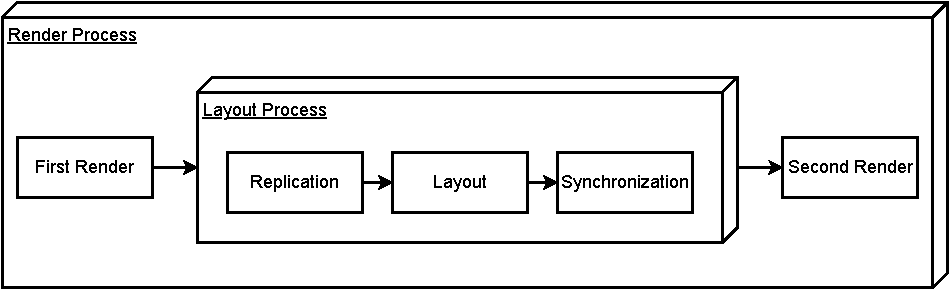
\includegraphics[keepaspectratio,width=\linewidth,height=\fullh]{diagrams/respvis-render-process.pdf}
\caption[Render Process When Using the Layouter]{
  This diagram shows the three phases of the render process when using the RespVis Layouter. 
  During the first render phase, every element that affects the layout needs to be rendered.
  The layout phase of the render process is equivalent to the layout process described in Figure~\ref{fig:LayoutProcess}.
  In this phase, the Layouter calculates the final positions and sizes of laid-out elements and stores them in attributes on these elements.
  During the second render phase, the boundary informations calculated in the previous phase is utilized to rerender all elements of the visualization at their final positions with their final dimensions.
  \imgcredit{Image created by the author of this thesis using \href{https://www.diagrams.net/}{diagrams.net}.}
}
\label{fig:RenderProcess}
\end{figure}


\subsection{Axes}

Axes are implemented in the \code{axis.ts} file in the Core Module and are used to visualize scales that map abstract values to spatial dimensions.
Currently, only Cartesian Axes, which are distinguished by their position relative to a visualization's draw area, are provided by RespVis because only Cartesian Charts have been implemented so far.
The implementation has so far been focused on Left and Bottom Axes because they are the most commonly encountered types of Cartesian Axes and cover most use cases. 
An Axis consists of ticks, an optional title, and an optional subtitle, where the ticks of an Axis are the actual visualization of the Axis' scale, and the title and subtitle can be specified for additional description.
An example of what a rendered Left and Bottom Axis might look like can be seen in Figure~\ref{fig:Axes}. 

\begin{figure}[tp]
\centering
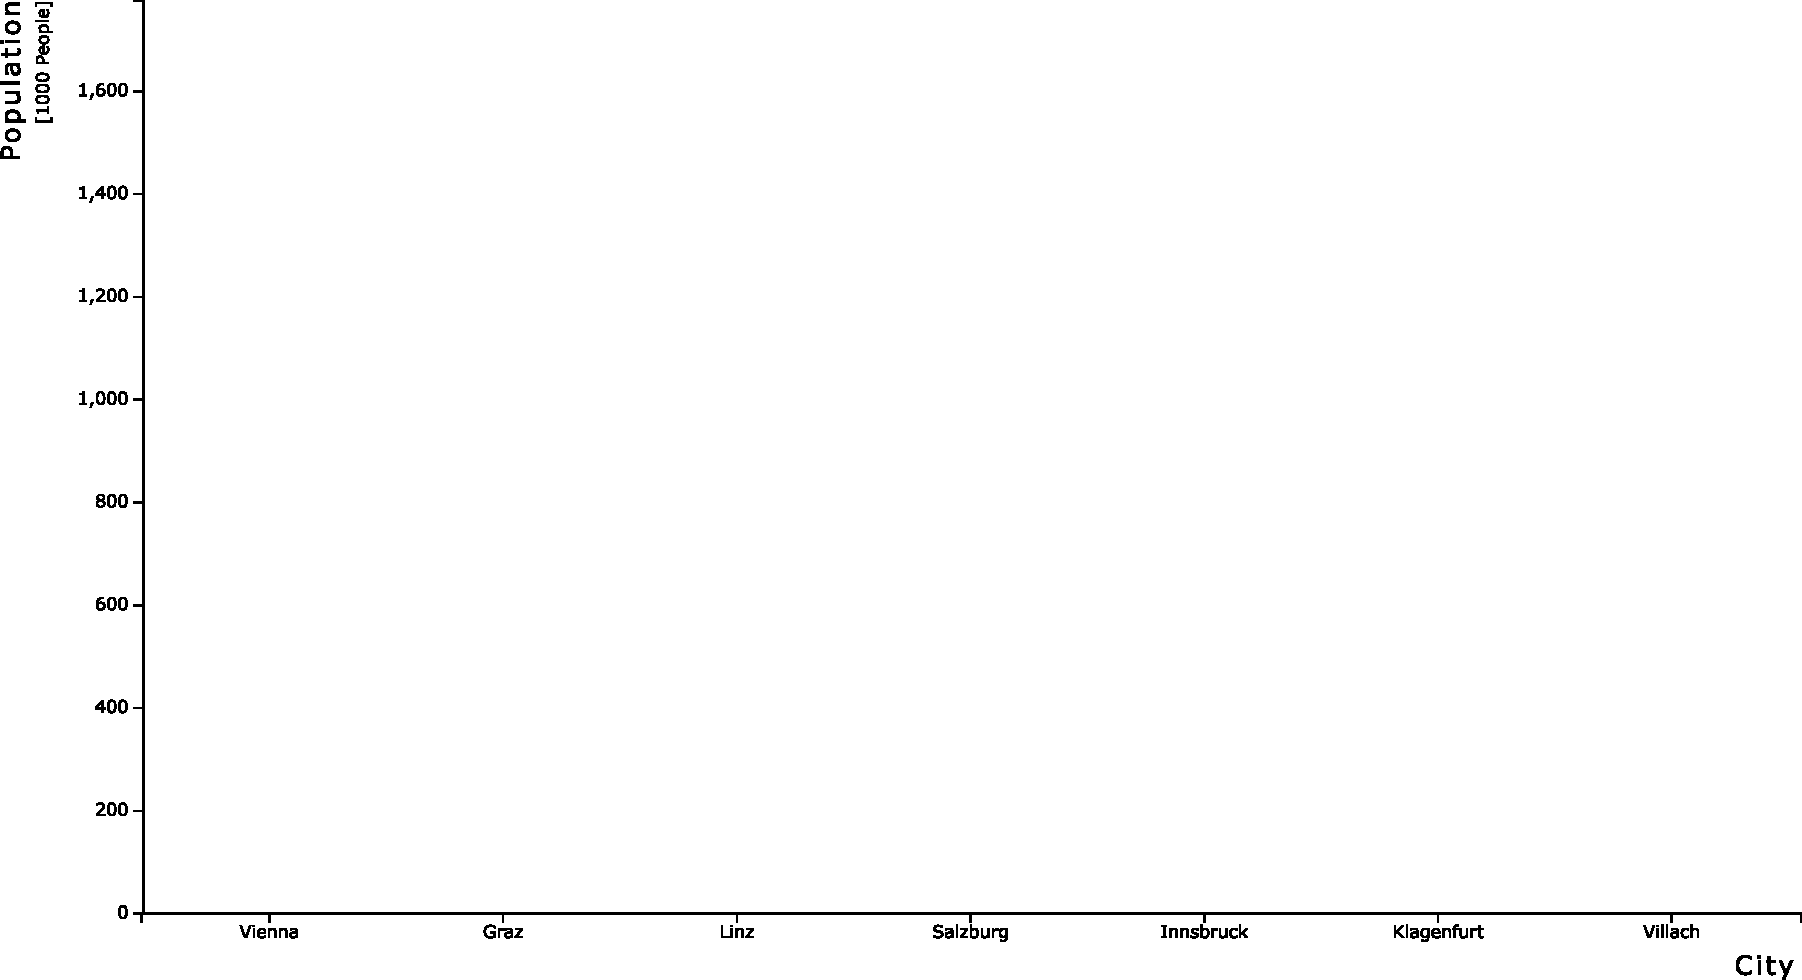
\includegraphics[keepaspectratio,width=\linewidth,height=\fullh]{diagrams/axes.pdf}
\caption[RespVis Axis Components]{
  This figure shows how a rendered Left and Bottom Axis may look like.
  The Left Axis consists of a title, subtitle, and ticks, whereas the Bottom Axis only consists of ticks and a title. 
  \imgcredit{Image created by the author of this thesis using RespVis and \href{https://inkscape.org/}{Inkscape}.}
}
\label{fig:Axes}
\end{figure}
  

The \code{Axis} interface describes the shape of a data object with which an Axis can be configured.
It includes a \code{scale} property, which represents the scale that has to be visualized, the \code{title} and \code{subtitle} string properties, and the \code{configureAxis} function property, which can be used to configure the underlying D3 axis before rendering it.  
Like most other components, axis components consist of two main functions: a data creation function and a render function.
The \code{axisData} function is used to create an \code{Axis} data object from a \code{Partial<Axis>} object parameter where all non-set but required properties are filled with default values.
The \code{axisBottomRender} and \code{axisLeftRender} functions are used to render a Left and Bottom Axis in a composite element on which an \code{Axis} data object has been bound. 
An Axis' root element is a CSS Grid container and defines the layout of the title, subtitle, and ticks elements.
The default configuration of a Left Axis positions these elements in a three-column layout in which the title, subtitle, and ticks elements are placed in this order from left to right.
For a Bottom Axis, the default configuration positions the same elements in a three-row layout in which the ticks, title, and subtitle elements are placed in this order from top to bottom.
Furthermore, the title and subtitle elements of a Left Axis are oriented vertically to save horizontal space using the \code{textOrientation} utility function.
The RespVis Axis Components internally use the \code{axisBottom} and \code{axisLeft} functions from the D3 Axis Module \parencite{D3Axis} to render the ticks of an Axis.
Since these D3 functions use attributes to position and style elements, as many of these attributes as possible must be removed directly after the ticks have been rendered to enable their configuration via CSS.  

\subsection{Chart}

Charts are high-level components that represent a complete visualization with Axes, Legends, and Series.
An example of a rendered RespVis Chart that includes two Axes, a Grouped Bar Series, a Label Series, and a Legend can be seen in Figure~\ref{fig:Chart}.
A Chart is typically rendered in the root \code{<svg>} element of an SVG document that has at least the \code{chart} class set in its \code{class} attribute and the appropriate SVG namespace set in its \code{xmlns} attribute.
These attributes can be set in more specific Chart Components either manually or via the \code{chartRender} function from the \code{chart.ts} file in the Core Module, which only sets these attributes.


\begin{figure}[tp]
  \centering
  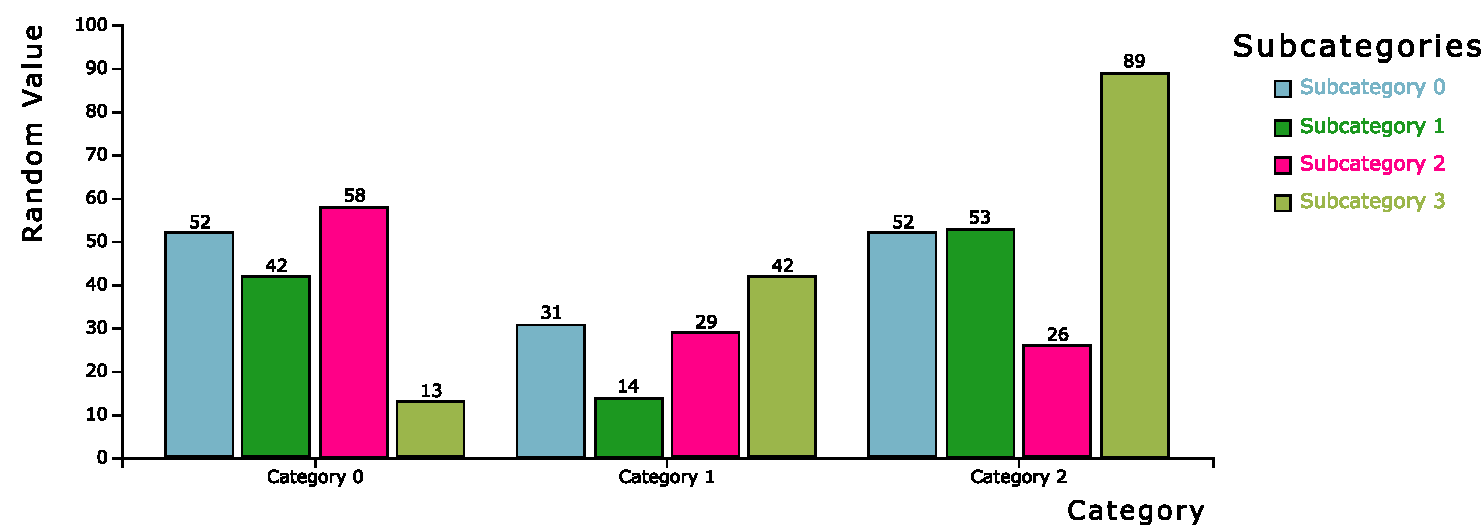
\includegraphics[keepaspectratio,width=\linewidth,height=\fullh]{diagrams/chart.pdf}
  \caption[Chart Example]{
    An example of a Chart that contains two Axes, a Grouped Bar Series, a Label Series and a Legend.
    \imgcredit{Image created by the author of this thesis.}
  }
  \label{fig:Chart}
\end{figure}

As mentioned previously, RespVis currently contains only the implementations of Cartesian Charts, which visualize data in a Cartesian coordinate system.
The implementation of the base functionality of such Cartesian Charts is located in the \code{chart-cartesian.ts} file in the Core Module. 
The \code{ChartCartesian} interface describes a data object for the configuration of Cartesian Charts via the \code{xAxis} and \code{yAxis} \code{Axis} properties which describe the X and Y Axes of the Chart respectively.
Transposing Axes is a useful pattern to improve the responsiveness of visualizations and can be configured using the \code{flipped} boolean property of \code{ChartCartesian} data objects.
If the \code{flipped} property is set to \code{false}, the \code{xAxis} object is used to configure the Bottom Axis and the \code{yAxis} object is used to configure the Left Axis. 
If it is set to \code{true}, it is the other way around.

The \code{chartCartesianData} function is used to create a \code{ChartCartesian} data object.
This function gets a partial data object with only those properties set that are of interest to the calling code, and all non-set properties are filled with default values.
The default values of the \code{xAxis} and \code{yAxis} properties are set by the \code{axisData} function from the Axis Module and the \code{flipped} property is initialized to \code{false}.

The rendering of Cartesian Charts is split into two functions that have to be called separately because not all parts of a Cartesian Chart can be rendered simultaneously.
The general structure of a Chart must be rendered before anything else can be rendered, as this includes the draw area container element into which individual Series Components are rendered.
A Chart's Axes need fully initialized scales to be rendered correctly.
However, the range of a scale, i.e. the range of values into which abstract values are mapped, depends on the size of the draw area and is only set during the render function of the individual Series Components.    
Therefore, the Axes of a Cartesian Chart must be rendered after Series Components to ensure fully initialized scales.

The structure of a Cartesian Chart is rendered with the \code{chartCartesianRender} function, which sets the necessary attributes and classes on the root element and attaches the draw area \code{<svg>} element to it.
The draw area is the container element into which the Series Components of a Chart are rendered.
An \code{<svg>} element without actual content is not able to catch input events, which means that it would, for example, not be possible to capture scroll events to control a zoom interaction when the cursor is over the empty area of the draw area.
To counteract this, a transparent \code{<rect>} background element that fills the whole draw area is added, which allows capturing input events even in empty areas.

The \code{chartCartesianAxesRender} function is used to render the Axes of a Cartesian Chart.
This function must only be called on elements with a bound \code{ChartCartesian} data object and after the scales that are to be visualized by the Axes have been fully initialized.
Charts must first render the Chart's structure using the \code{chartCartesianRender} function, followed by the desired Series Components, and only after those the Chart's Axes can be rendered using the \code{chartCartesianAxesRender} function.
The \code{chartCartesianAxesRender} function creates two \code{<g>} elements and renders Left and a Bottom Axes in them.
Depending on whether the \code{flipped} property in the bound data object is set to \code{true} or \code{false}, the \code{xAxis} data object is used to configure the Bottom or Left Axis and the \code{yAxis} data object is used to configure the other one.
After the Axes are rendered, the \code{x-axis} class is set on the one the \code{x-axis} data object is bound to, and the \code{y-axis} class is set on the other one.

The elements of a Cartesian Chart are positioned using a CSS Grid layout.
By default a grid is created which defines the \code{axis-left}, \code{axis-bottom}, \code{draw-area}, and \code{legend} areas.
Most rows and columns of this grid are sized to fit their content, with the only exception being the row and column containing the draw area, which is set to fill the remaining space not occupied by the other rows and columns.
The default CSS configuration of a Cartesian Chart positions an eventual legend to the right of the draw area, but this can be changed by either adjusting the grid directly via CSS or activating one of the preconfigured positions via the \code{data-legend-position} attribute.
To simplify setting the \code{data-legend-position} attribute, the \code{chartLegendPosition} function can be used, which sets this attribute to the value of a passed \code{LegendPosition} enum parameter.


\subsection{Chart Window}

Chart Windows are implemented in the \code{chart-window.ts} file in the Core Module and are wrapper components around Charts that render a Chart inside a Layouter and decorate it with a Toolbar.
These components represent an even higher-level layer than Charts and are used to manage their rendering process and configuration.
In most other visualization libraries, Charts are provided as the highest level of components that can be configured, which typically means that additional HTML elements for the runtime configuration of Charts have to be created and managed by the embedding web page itself.
Chart Windows are rendered with the \code{chartWindowRender} function on HTML \code{<div>} elements containing a Chart's SVG document.
Their structure consists of a \code{<div>} element in which the Toolbar is rendered, and of another \code{<div>} element on which a Layouter is initialized and which holds the wrapped Chart's SVG document. 
An example of a Chart Window with an expanded Tool Menu containing two Nominal Filtering Tools and an SVG Download Tool can be seen in Figure~\ref{fig:ChartWindow}.


\begin{figure}[tp]
  \centering
  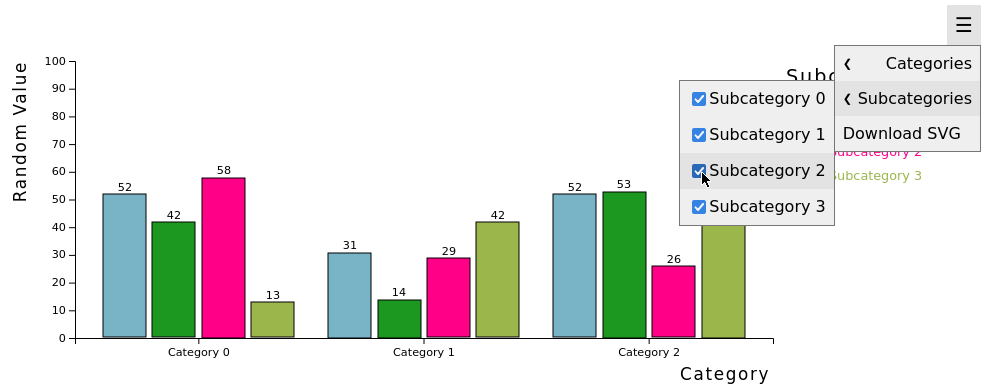
\includegraphics[keepaspectratio,width=\linewidth,height=\fullh]{images/chart-window.png}
  \caption[Chart Window Example]{
    An example of a Chart that is wrapped in a Chart Window.
    The Tool Menu has been expanded by hovering over it, and the menu entries of two Nominal Filtering Tools and the SVG Download Tool can be seen inside.
    \imgcredit{Image created by the author of this thesis.}
  }
  \label{fig:ChartWindow}
\end{figure}


Currently, the Toolbar only contains the Tool Menu, a dropdown menu into which individual tools are added as menu items or as submenus.
Dropdown menus are created with the \code{menuDropdownRender} function and consist of a title and a container for menu items.
The current dropdown menu implementation uses no JavaScript and simply shows menu items via CSS when there is a hover interaction. 
The Tool Menu is created with the \code{menuToolsRender} function, which internally uses the \code{menuDropdownRender} function to initialize it as a dropdown menu.

The Core Module provides various tools that can be added to the Tool Menus of Chart Windows.
One of these tools is the Nominal Filtering Tool which is located in the \code{tools/tool-filter-nominal.ts} file of the Core Module.
This tool is used to filter a nominal data dimension of a visualized dataset via a dropdown menu that includes a Checkbox Series.
Nominal data, in contrast to ordinal or quantitative data, consists only of labels that do not have a quantitative value assigned to them and therefore cannot be ordered or sorted.
The data object for the configuration of a Nominal Filter Tool is described by the \code{ToolFilterNominal} interface, which contains properties to specify the title of the dropdown menu, the individual options to be filtered, and the keys of these options. 
The \code{toolFilterNominalData} function is used to create a data object of type \code{ToolFilterNominal} from a partial input object where undefined properties are being filled with default values.
Nominal Filtering Tools can then be rendered on elements with bound \code{ToolFilterNominal} data objects using the \code{toolFilterNominalRender} function, which internally uses the \code{menuDropdownRender} function to initialize a dropdown menu into which the checkboxes representing the individual options of the filter are rendered as menu items.

Checkbox Series are implemented in the \code{series-checkbox.ts} file in the Core Module and they render series of checkboxes consisting of checkbox \code{<input>} elements with associated \code{<label>} elements.
They are configured using data objects in the form of the \code{SeriesCheckbox} interface, which contains properties to determine the type of checkbox container elements and the labels of checkboxes.
A data object of this type can be created with the \code{seriesCheckboxData} function, which creates a complete object from a partial one.
Checkbox Series are rendered using the \code{seriesCheckboxRender} function, which generates individual checkboxes using a data join that join requires an array of \code{Checkbox} data objects so that a single data object can be bound to each checkbox.
Individual \code{Checkbox} data objects contain all data needed to render a single checkbox and are created by transforming the \code{SeriesCheckbox} data objects bound on the Series' root element.
Single checkboxes consist of a container element, an \code{<input>} checkbox element, and a \code{<label>} element.
In order to semantically assign the \code{<label>} elements to their \code{<input>} elements, the \code{for} attributes on \code{<label>} elements must be set to the ids of their corresponding \code{<input>} elements.
This requires assigning unique ids to \code{<input>} elements, which are generated via the \code{uuid} function and set as \code{id} attributes on the \code{<input>} elements and as \code{for} attributes on \code{<label>} elements when the checkbox is first created.
The \code{uuid} function is an alias for the \code{v4} function from the \code{uuid} npm package \parencite{UUIDPackage} and is used to generate UUIDs (Universally Unique IDentifiers) \parencite{UUIDRFC} of the fourth version, which are very likely to be unique and therefore can be safely used as values for \code{id} attributes.

The SVG Download Tool is implemented in the \code{tools/tool-download-svg.ts} file of the Core Module and is included by default in every Chart Window.
SVG documents embedded in HTML documents cannot as easily be downloaded by users as raster images, which can simply be downloaded with native browser tools. 
Instead, SVG documents must be encoded in \code{Blob} objects and then set as as object URLs in the \code{href} attributes of \code{<a>} elements.
However, since the presentation of RespVis visualizations is mainly configured using CSS, the active CSS properties must first be converted to attributes before the SVG document can be downloaded.
For this, a clone of the whole SVG document is made to set attributes on the cloned elements without affecting the rendered visualization.
After the document has been cloned, attributes reflecting the active CSS configuration of the original elements are set on cloned elements.
The active CSS configuration of the original elements is calculated using the \code{elementComputedStyleWithoutDefaults} utility function, which yields a list of CSS properties and their values, only containing properties that are not set to defaults.  
After setting all the necessary attributes on cloned elements, the string representation of the cloned document is calculated using the \code{Element.innerHTML} property and encoded in a \code{Blob} object with the content type \code{image/svg+xml}.
At present, the string representation of the SVG document is not further processed or formatted, which results in a rather difficult-to-read file and which will be improved in future work. 
The \code{Blob} object containing the SVG document is further transformed into an object URL via the \code{URL.createObjectURL} method and set in the \code{href} attribute of a newly created \code{<a>} element.
This newly created \code{<a>} element is then briefly attached to the \code{<body>} element of the active HTML document and clicked using the \code{Element.click} method, which initiates the download of the final prepared SVG document.
Download SVG Tools can be rendered as menu items in a Chart Window's Tool Menu with the \code{toolDownloadSVGRender} function, which initializes them and triggers the download of the SVG document embedded in the Chart Window when the user clicks on the menu item.

\section{Legend Module}

The Legend Module in the \code{src/lib/legend/} directory consists only of the \code{legend.ts} file, which contains the implementation of a Legend Component.
Legends are used to visualize scales whose abstract values are not mapped to spatial dimensions in a coordinate system but to other visual properties such as colors, shapes, or sizes.
The Legend implemented in this module illustrates such scales by creating labeled, configurable symbols for every mapping and, therefore, this component is best suited for the visualization of discrete value mappings.
Continuous data dimensions can still be visualized with this component, but they must be approximated by dividing the continuous domain of values into equal discrete steps.
An example demonstrating the use of the Legend Module can be found in the \code{legend.html} file in the \code{src/examples/} folder, and an excerpt of this example can be seen in Listing~\ref{list:Legend} with its rendering shown in Figure~\ref{fig:Legend}.

\begin{samepage}
\lstinputlisting[%
  float=tp,
  aboveskip=\floatsep,
  belowskip=\floatsep,
  xleftmargin=0cm,              % no extra margins for floats
  xrightmargin=0cm,             % no extra margins for floats
  %
  basicstyle=\footnotesize\ttfamily,
  frame=shadowbox,
  numbers=left,
  label=list:Legend,
  caption={[Source Code of Legend Example]%
    The source code of the example implemented in the \code{legend.html} file in the \code{src/examples/} directory.
    When executed, this code results in the three Legends seen in Figure~\ref{fig:Legend}.
    Non-essential parts of the source code have been removed to focus on Legend-related configurations.
    The horizontal Legend has been configured with the same data object as the rectangle symbol Legend, but the items of the horizontal Legend have been laid out horizontally via the \code{flex-direction: row} CSS property.
  },
]{listings/legend.html}
\end{samepage}

\begin{figure}[tp]
\centering
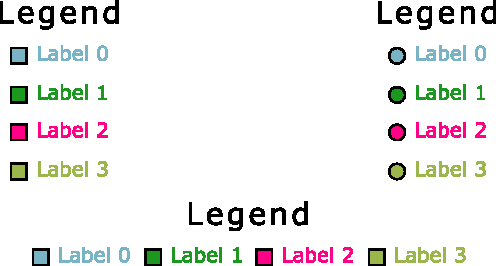
\includegraphics[keepaspectratio,width=\linewidth / 2,height=\fullh]{diagrams/legend.pdf}
\caption[Legend Example]{
  These are the three resulting Legends that are being rendered by the source code in Listing~\ref{list:Legend}.
  One Legend has been configured to have rectangles as symbols, one has been configured to have circles as symbols, and the last one has been configured with rectangle symbols but with horizontally laid out items.
  \imgcredit{Image created by the author of this thesis.}
}
\label{fig:Legend}
\end{figure}

A data object for the configuration of a Legend is defined by the \code{Legend} interface, which contains properties to describe the title, labels, and symbols of a Legend.
Symbols are configured via functions that take the boundaries calculated by the Layouter into account to set the \code{d} attributes of \code{<path>} elements.
Legend symbols are rendered as \code{<path>} elements because these enable the rendering of arbitrary symbols that can be changed dynamically, whereas the usage of \code{<rect>} or \code{<circle>} elements would be much more restricting.
A disadvantage of using \code{<path>} elements is that, since they require manual configuration of exact shapes via path definition strings, their usage is more tedious than the usage of more restricted SVG elements, and they require slightly more annotation effort when it comes to accessibility.
Colors of individual items in a Legend are indirectly configured via \code{data-style} attributes on items whose values are specified in the \code{Legend} data objects.
Some style classes, such as the \code{categorical-x} classes for categorical styling, are already provided by RespVis and handled in the library's distributable CSS file.
Furthermore, custom style classes can easily be added by simply handling them in user-specified CSS rules.
\code{Legend} data objects can be created with the \code{legendData} function, which receives a partial input object in which the properties that are not of interest to the calling code are not required to be set and are populated with default values.

A Legend is rendered into elements that have a \code{Legend} data object bound on them using the \code{legendRender} function.
This function sets the \code{legend} class on the root element, attaches a \code{<text>} element with which the title of the Legend is shown, and attaches a \code{<g>} element into which the individual items of the Legend are rendered via a data join.
To perform the data join with which the items of the Legend are created, one \code{LegendItem} data object per item to be rendered is needed to describe individual legend items, and these are generated via transformation of the bound \code{Legend} data object.
Via a data join with these data objects, one \code{<g>} element with the \code{legend-item} class is created for every legend item, to which a \code{<path>} element for the symbol and a \code{<text>} element for the associated label are attached.
The operations performed during this data join can be directly modified via the custom \code{enter}, \code{update}, and \code{exit} events, which are dispatched on the root element of the Legend and which respectively contain the data join's enter, update, or exit Selection in a property of the event object.
Also, the \code{legendRender} function sets the \code{data-style} and \code{data-key} attributes on the legend item elements to values configured on the bound \code{Legend} data object.

\section{Tooltip Module}
\label{sec:TooltipModule}

Tooltips display additional contextual information that is too expansive to be shown all the time because the more information a visualization shows simultaneously, the more cognitive effort is required to interpret it.
Detailed information that may be valuable but not necessary for understanding a visualization's core message is only shown via a Tooltip when the user interacts with an element in whose context this information stands.
Due to Tooltips only being explicitly shown by users, they may overlap and cover other elements of a Chart that would otherwise be too important to hide.
An example of a Bar Chart in which additional information is displayed via a Tooltip can be seen in Figure~\ref{fig:Tooltip}.

\begin{figure}[tp]
\centering
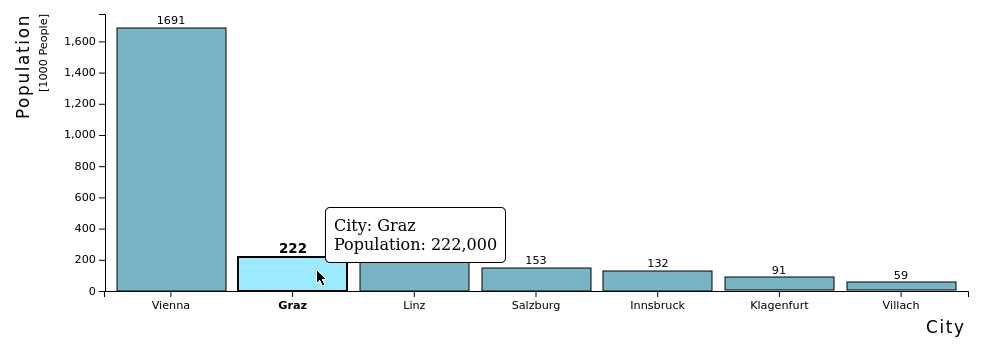
\includegraphics[keepaspectratio,width=\linewidth,height=\fullh]{images/tooltip.png}
\caption[Tooltip Example]{
  This Figure shows a Bar Chart with an active Tooltip that displays additional information of the data record associated with an individual bar.
  Due to the Tooltip only being visible during interaction with a context element, it may overlap and cover other important parts of the Chart.
  \imgcredit{Image created by the author of this thesis.}
  }
  \label{fig:Tooltip}
\end{figure}
  
The Tooltip Module is located in the \code{src/lib/tooltip/} directory of the RespVis library and contains the implementation of Tooltips and utility functions to simplify the configuration of Tooltips on Series Components.
Tooltips are merely HTML \code{<div>} elements with the \code{tooltip} class that are styled via CSS and that can be initialized with the \code{tooltip} function.
Their visibility, position, and content is controlled via the \code{tooltipShow}, \code{tooltipHide}, \code{tooltipPosition}, and \code{tooltipContent} functions in the \code{tooltip.ts} file of the Tooltip Module.
Due to the support of multiple simultaneous Tooltips, all of these functions have to be passed the Tooltip element they should affect or a \code{null} value in place of it to indicate usage of a default element attached to the body of the active document.
Tooltips are shown and hidden via the \code{tooltipShow} and \code{tooltipHide} functions, which respectively add or remove the \code{show} class to the classes of the Tooltip element.
The actual showing and hiding is done in CSS by setting the \code{opacity} property of the element depending on whether or not the \code{show} class is set.
Positions of Tooltips are configured via the \code{tooltipPosition} function. 
This function calculates positions through an anchor position in viewport coordinates and a directional offset from that anchor.
Specifying the anchor position is necessary, but the directional offset can be omitted to have a sensible one chosen by the \code{tooltipPosition} function so that the Tooltip is always placed inside the visible area of the browser.
The actual positioning is again done in CSS by setting a combination of the \code{left}, \code{right}, \code{bottom}, and \code{top} properties depending on the offset direction of the Tooltip.
A Tooltip's content can be set with the \code{tooltipContent} function which sets the Tooltip's inner HTML to the HTML string passed to the function.

Apart from Tooltips, the Tooltip Module also contains utility functions that aim to simplify the setup and handling of Tooltips on different Series Components such as Bar or Point Series.
Interfaces describing the data objects of Series Components can inherit from the \code{SeriesConfigTooltips} interface to add additional properties for the configuration of Tooltips to these data objects. 
Among these properties is a property to enable the Tooltips of the Series and properties to specify the contents and positions of individual Tooltips based on their associated context-element and the current cursor position.
In addition to the \code{SeriesConfigTooltips} interface, the \code{seriesConfigTooltipsHandleEvents} function is provided to automatically set \code{mouseover}, \code{mousemove}, and \code{mouseout} event listeners on Series to automatically update the visibility, content, and position of Tooltips based on the \code{SeriesConfigTooltips} properties stored in the Series' data object.
The usage of these utilities is optional, and Series Components are free to provide their own properties for the configuration of Tooltips and their handling.
However, for consistency reasons, the way of configuring Tooltips should not differ too much between different types of Series Components, and therefore it is recommended to use the utilities provided here unless there is a good reason not to.


\section{Bar Module}

Bar Charts are used to compare the values of quantitative variables that are uniquely associated with distinct values of qualitative variables by visualizing these variables as rectangles whose lengths are proportional to the quantitative values.
An example of variables that can be plotted using a Bar Chart would be countries with their populations, people with their ages, and browsers with their market shares.
Bar Charts have already been in use for quite a long time, with one of the earliest documented occurrences being \textcite{CommercialAndPoliticalAtlas}, and they are still among the most frequently encountered types of visualizations in the modern web.

The bars of a Bar Chart can either be horizontally or vertically oriented.
In Horizontal Bar Charts, sometimes also called Row Charts, categories are spread in equal intervals across the Y-Axis to define the positions and heights of bars, and the associated values of categories are mapped on the X-Axis to determine their widths. 
Conversely, in Vertical Bar Charts, sometimes also called Column Charts, categories are spread in equal intervals across the X-Axis to determine the positions and widths of bars, and the values of categories are mapped on the Y-Axis to determine their heights.
Horizontal Bar Charts are better suited for display in narrow contexts than Vertical Bar Charts because category labels can be positioned more easily without having to rotate them and because these Charts can be vertically extended by having the user scroll vertically, which is strongly preferable to horizontal scrolling. 

The Bar Module is located in the \code{src/lib/bars/} directory of the RespVis library and contains components to create Single-Series, Grouped Multi-Series, and Stacked Multi-Series Bar Charts that can be used in different situations.
For every type of Bar Chart, the Bar Module provides a respective Series Component to render only the actual bars, a Chart Component to render a full Chart including bars, axes, and possible legends, and a Chart Window Component to render a full Chart embedded into a Layouter with additional tools provided via a Toolbar.
Higher-level components are more convenient to use, but they also impose more assumptions, and therefore restrictions, on lower-level components contained within them.
The implementations of the different types of Bar Charts and when which type is best used is described in the following sections.

\subsection{Basic Bars}

\TODO{Is "Basic Bars" a good name? Maybe "Single Bars" or "Bars" or something else?}

\TODO{Add figure of vertical and horizontal bar charts (subfigures?)}

basic bar charts, manchmal auch single-series bar charts genannt, werden verwendet um unterschiede einer quantitativen dimension verschiedener kategorien eines kategorischen datensatzes zu verdeutlichen.
von jedem dateneintrag wird jeweils eine kategorische und eine quantitative dimension als eine bar visualisiert, wobei die zu visualisierenden kategorien eindeutig auf einen quantitativen wert gemapped werden koennen muessen.
die kategorien eines bar charts werden ueber eine band scale auf raeumliche dimensionen gemapped.
eine band scale wird verwendet um werte gleichmaessig auf gleich grosse intervalle (baender) des verfuegbaren platzes aufzuteilen. 
der abstand zwischen den einzelnen intervallen ist konfigurierbar.
die breite der zu rendernden bars ergibt sich durch die anzahl der kategorien, dem bereich auf welchen sie ueber die band scale aufgeteilt werden sollen, und dem abstand zwischen den bars. 
die quantitativen werte, welche die laenge der individuellen bars bestimmen, werden ueber eine continuous scale auf raemliche dimensionen gemapped.
eine continuous scale bildet abstrakte quantitative werte ueber eine kontinuierliche interpolationsfunktion auf den bereich zwischen zwei extemen ab.
in den meisten faellen kommt eine lineare interpolation ueber eine linear scale zur anwendung.
es steht dem author einer visualisierung jedoch frei eine andere form der interpolation, wie zum beispiel eine logarithmische funktion ueber eine logarithmic scale, zu waehlen. 

die lowest-level komponente die fuer das rendern eines bar charts notwendig ist ist eine bar series.
eine bar series ist eine sammlung von \code{<rect>} elementen welche die bars innerhalb der draw area eines bar charts representieren.
die implementierung der bar series komponente befindet sich in der \code{series-bar.ts} datei des bar moduls.
das datenobjekt fuer die konfiguration einer bar series wird ueber das \code{SeriesBar} interface beschrieben.
diese interface beschreibt ein objekt mit den \code{categories}, \code{values}, \code{categoryScale}, \code{valueScale}, \code{flipped}, \code{styleClasses}, und \code{keys} eigenschaften.
zusaetzlich zu diesen eigenschaften wird die konfiguration von tooltips ueber die eigenschaften des \code{SeriesConfigTooltips} interface, welches in Section~\ref{sec:TooltipModule} beschrieben wird, ermoeglicht.
die \code{categories} und \code{values} eigenschaften sind arrays welche die individuellen kategorien und deren quantitative werte repraesentieren.
das mapping der kategorischen und quantitativen werte auf raeumliche dimensionen wird ueber die \code{categoryScale} und \code{valueScale} eigenschaften bestimmt.
ob vertikale oder horizontale bars gerendert werden haengt von dem wert der \code{flipped} eigenschaft ab, wobei ein wert von \code{false} fuer vertikale bars und ein wert von \code{true} fuer horizontale bars steht.
die \code{data-style} attribute, welche die farbe von bars bestimmen, und die \code{data-key} attribute, welche zur identifikation von zusammengehoerenden elementen verwendet werden, werden ueber die \code{styleClasses} und \code{keys} eigenschaften bestimmt.
ein mit standardwerten initialisiertes \code{SeriesBar} datenobjekt kann mit der \code{seriesBarData} funktion von einem partiellen input objekt erzeugt werden.
diese datenobjekte koennen an \code{<svg>} oder \code{<g>} elemente gebunden werden in welche dann eine bar series mit der \code{seriesBarRender} funktion gerendert werden kann.
die individuellen bar elemente werden ueber einen data join mit einem array an \code{Bar} datenobjekten erzeugt, welches durch transformation des gebundenen \code{SeriesBar} datenobjektes berechnet wird.
die position und groesse der bars wird mithilfe der beiden scales berechnet deren output values auf die dimensionen der bounding box des series elementes gemapped werden, welche vom Layouter berechnet und im \code{bounds} attribut gespeichert wurden.
jede bar hat eine enter und exit transition und ihre position und groesse wird ueber eine update transition zwischen aktuellen und neuen werten interpoliert.
diese transitions erleichtern es aenderungen in den visualisierten daten nachzuvollziehen und fuehren zu einer verbesserung der user experience.
wie bei alle anderen series komponenten, werden die enter, update, und exit events mit der jeweiligen Selection des bar data joins auf dem root element der series dispatched um das injezieren von eigenem verhalten in die verschiedenen phasen des data joins zu ermoeglichen. 

die implementierung von bar charts befindet sich in der \code{chart-bar.ts} datei im bar modul. 
bar charts sind kartesische charts die eine bar series mit optionalen labels in ihrer draw area rendern.
das \code{ChartBar} interface beschreibt die form von datenobjekten fuer die konfiguration von bar charts.
es beinhaltet alle eigenschaften der \code{ChartCartesian} und \code{SeriesBar} interfaces und fuegt zusaetzliche eigenschaften zur konfiguration von bar labels hinzu. 
ein mit standardwerten initialisiertes datenobjekt vom typ \code{ChartBar} kann mit der \code{chartBarData} funktion von einem partiellen input objekt erzeugt werden.
nachdem solch ein datenobjekt auf einem \code{<svg>} oder \code{<g>} element gebunden wurde, kann ein bar chart mit der \code{chartBarRender} funktion in dieses element gerendert werden.
diese funktion initialisiert einen kartesischen chart, initialisiert und rendert eine bar series und eine optionale label series in der draw area des charts, und rendert die scales mit welchen die bar series gerendert wurde als left und bottom axes des charts. 
weiters werden \code{mouseover} event listener an die bar series angehaengt die fuer das hervorheben von bars und den dazugehoerigen ticks auf der category axis zustaendig sind.

ein bar chart window ist die highest-level komponente die verwendet werden kann um einen bar chart zu rendern der in ein Layouter element eingebettet wird um dessen elemente ueber CSS zu positionieren.
ueber die toolbar des bar chart windows koennen die kategorien des bar charts gefiltert und das SVG dokument des bar charts gedownloaded werden.
das datenobjekt fuer die konfiguration eines bar chart windows wird durch das \code{ChartWindowBar} interface beschrieben.
dieses interface erbt vom \code{ChartBar} interface und beinhaltet dadurch alle eigenschaften die fuer die konfiguration des darunterliegenden bar charts benoetigt werden.
zusaetzlich zu diesen, werden weitere eigenschaften fuer das filtern von kategorien, wie etwa die derzeit aktiven kategorien und das verhalten der value scale, zur verfuegung gestellt.
die \code{chartWindowBarData} funktion kann verwendet werden um ein datenobjekt fuer die konfiguration eines bar chart windows von einem partiellen input objekt zu erzeugen bei welchem die nicht definierten werte mit standardwerten initialisiert werden.
mit der \code{chartWindowBarRender} funktion kann ein bar chart window in einem \code{<div>} element auf welchem ein angemessenes datenobjekt gebunden is gerendert werden.
diese funktion rendert die toolbar mit den kategorie filter und SVG download tools, initialisiert den eingebetteten chart mit den gefilterten werten des chart window datenobjektes, und rendert den chart, entsprechend des render prozesses definiert in Section~\ref{sec:Layouter}, zweimal mit einem layout computation schritt dazwischen.
standardmaessig wird das chart window nicht automatisch rerendert wenn sich die groesse des viewports aendert oder wenn die aktiven kategorien gefiltert werden.
das rerendern bei viewport groessenaenderungen kann ueber einen \code{resize} event listener auf dem chart window root element implementiert werden in welchem die chart window render funktion erneut aufgerufen wird nachdem das gebundene datenobjekt angemessen an die neuen dimensionen des viewports angepasst wurde.
das bar chart window sendet ein \code{categoryfilter} event mit den derzeit aktiven kategorien immer wenn kategorien ueber das filter tool aktiviert oder deaktiviert werden.
um den bar chart auf die neue filterkonfiguration anzupassen muss ein \code{categoryfilter} event listener implementiert werden welcher die aktiven kategorien im datenobjekt des chart windows aktualisiert und das chart window rerendert.
muessen keine speziellen konfigurationen bei aenderung der viewport groesse oder des kategoriefilters durchgefuehrt werden, koennen die \code{chartWindowBarAutoResize} und \code{chartWindowBarAutoFilterCategories} funktionen verwendet werden um \code{resize} und \code{categoryfilter} event listener an das chart window anzuhaengen die das standardverhalten implementieren.
ein simples beispiel dafuer wie ein skalierendes bar chart window erzeugt werden kann welches das filtern von kategorien erlaubt ist in Listing~\ref{list:BarChartWindow} ersichtlich.
die resultierende visualisierung dieses codes kann in Figure~\ref{fig:BarChartWindow} gesehen werden.

\begin{samepage}
\lstinputlisting[%
  float=tp,
  aboveskip=\floatsep,
  belowskip=\floatsep,
  xleftmargin=0cm,              % no extra margins for floats
  xrightmargin=0cm,             % no extra margins for floats
  %
  basicstyle=\footnotesize\ttfamily,
  frame=shadowbox,
  numbers=left,
  label=list:BarChartWindow,
  caption={[Bar Chart Window Example]%
    The example source code that creates a Bar Chart Window.
    The Bar Chart Window is configured with the bound data object that is initialized via the \code{chartWindowBarData} function.
    After configuration, the Chart Window is rendered by the \code{chartWindowBarRender} function.
    Since no special responsive behavior is desired in this example, the default resize and category filter behavior is attached to the Chart Window via the \code{chartWindowBarAutoResize} and \code{chartWindowBarAutoFilterCategories} functions. 
  },
]{listings/bar-chart-window.js}
\end{samepage}
  

\begin{figure}[tp]
\centering
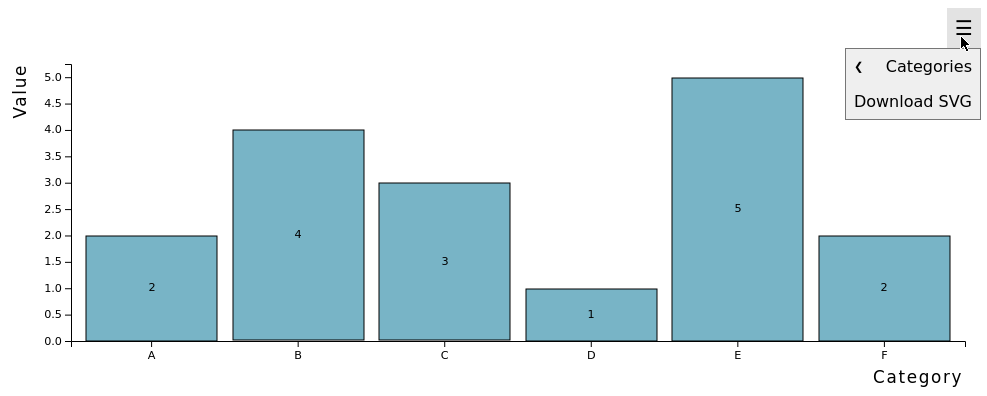
\includegraphics[keepaspectratio,width=\linewidth,height=\fullh]{images/bar-chart-window.png}
\caption[Bar Chart Window Example]{
  The resulting Bar Chart of the example code in Listing~\ref{list:BarChartWindow}. 
  \imgcredit{Image created by the author of this thesis using RespVis.}
}
\label{fig:BarChartWindow}
\end{figure}



\subsection{Grouped Bars}

ein grouped bar chart, manchmal auch clustered oder multi-series bar chart genannt, wird verwendet um mehrere quantitative dimensionen unterschiedlicher kategorien eines kategorischen datensatzes miteinander zu vergleichen.
in einem solchen chart wird fuer jede kategorie eine gruppe an bars gerendert deren laengen proportional zu den werten der unterschiedlichen quantitativen dimensionen sind.
die verschiedenen zu visualisierenden quantitativen dimensionen muessen miteinander vergleichbar sein und koennen als unterkategorien der einzelnen kategorien betrachtet werden.
wie bei basic bar charts werden auch hier die kategorien ueber band scales auf raeumliche dimensionen abgebildet.
der unterschied befindet sich darin dass bei grouped bar charts zwei verschiedene band scales zur anwendung kommen.
ueber die category scale wird der verfuegbare platz der draw area auf die anzahl der kategorien aufgeteilt und ueber die subcategory scale wird der platz innerhalb der daraus resultierenden gleich grossen intervalle auf die anzahl der unterkategorien aufgeteilt.
das abbilden von quantitativen werten auf raeumliche dimensionen wird wieder ueber eine continuous scale durchgefuehrt, wobei die selbe scale fuer jeden wert verwendet werden muss damit die werte miteinander vergleichbar sind.

fuer das rendering von grouped bar charts werden drei verschiedene komponenten zur verfuegung gestellt welche ihren gegenstuecken fuer das rendering von basic bar charts sehr aehnlich sind.
die grouped bar series ist die lowest-level komponente die dafuer gedacht ist eine sammlung an \code{<rect>} elementen, welche die jeweiligen werte und kategorien eines grouped bar charts representieren, in die draw area eines charts zu rendern.
der unterschied einer grouped bar series zu einer basic bar series ist dass zusaetzliche eigenschaften fuer die konfiguration der unterkategorien notwendig sind und dass manche bereits vorhandene eigenschaften hier zwei-dimensionale arrays erfordern um deren werte den hier zwei-dimensional (kategorie/unterkategorie) gruppierten bars zuzuordnen.
allen bars die der selben unterkategorie angehoeren werden die selben style klassen zugewiesen um die werte der einzelnen kategorien leichter miteinander vergleichen zu koennen.
ein grouped bar chart ist ein kartesischer chart mit einer grouped bar series und optionalen labels in seiner draw area, einer left und bottom axis die die scales der grouped bar series visualisieren, und einer legende die die unterkategorien des charts beschreibt.
ein solcher Chart implementiert ausserdem event listener auf unterschiedlichen elementen die das gemeinsame hervorheben von zusammengehoerenden bars, labels, category axis ticks, und legend items abwickeln.  
ein Grouped Bar Chart Window ist die highest-order komponente die verwendet werden kann um einen Grouped Bar Chart zu rendern.
diese komponente plaziert den Chart innerhalb eines Layouters und managed den render prozess der es erlaubt individuelle elemente ueber CSS zu positionieren.
weiters dekoriert ein solches Chart Window den Grouped Bar Chart mit einer toolbar in welcher sich ein SVG download tool und zwei filter tools befinden um die visualisierten kategorien und unterkategorien zu filtern.
die konfiguration des eingebetteten Charts mit den gefilterten eigenschaften des am Chart Window gebundenen datenobjektes wird von der render funktion des Grouped Chart Windows durchgefuehrt.
immer wenn der user mit den filter tools interagiert und die zusammenstellung der aktiven kategorien und unterkategorien veraendert werden die \code{categoryfilter} und \code{subcategoryfilter} events mit jeweils den neuen aktiven kategorien und unterkategorien ausgesandt.
der author der visualisierung kann entweder spezielles verhalten in eigenen resize und filter event listenern implementieren oder das standardverhalten ueber die zur verfuegung gestellten \code{chartWindowBarGroupedAutoResize}, \code{chartWindowBarGroupedAutoFilterCategories}, und \code{chartWindowBarGroupedAutoSubcategories} funktionen aktivieren.
der beispielcode um einen einfachen grouped bar chart zu erzeugen welcher sich an die groesse seines container elementes anpasst und in welchem die kategorien und unterkategorien ueber die toolbar gefiltert werden koennen befindet sich in Listing~\ref{list:GroupedBarChartWindow}.
die resultierende visualisierung dieses beispiels kann in Figure~\ref{fig:GroupedBarChartWindow} gesehen werden.  

\begin{samepage}
\lstinputlisting[%
  float=tp,
  aboveskip=\floatsep,
  belowskip=\floatsep,
  xleftmargin=0cm,              % no extra margins for floats
  xrightmargin=0cm,             % no extra margins for floats
  %
  basicstyle=\footnotesize\ttfamily,
  frame=shadowbox,
  numbers=left,
  label=list:GroupedBarChartWindow,
  caption={[Grouped Bar Chart Window Example]%
    The example source code that creates a Grouped Bar Chart Window.
    The Grouped Bar Chart Window is configured with the bound data object that is initialized via the \code{chartWindowBarGroupedData} function.
    After configuration, the Chart Window is rendered by the \code{chartWindowBarGroupedRender} function.
    Since no special responsive behavior is desired in this example, the default resize, category filter, and subcategory filter behavior is attached to the Chart Window via the \code{chartWindowBarGroupedAutoResize}, \code{chartWindowBarGroupedAutoFilterCategories}, and \code{chartWindowBarGroupedAutoFilterSubcategories} functions. 
  },
]{listings/grouped-bar-chart-window.js}
\end{samepage}
    
  
\begin{figure}[tp]
\centering
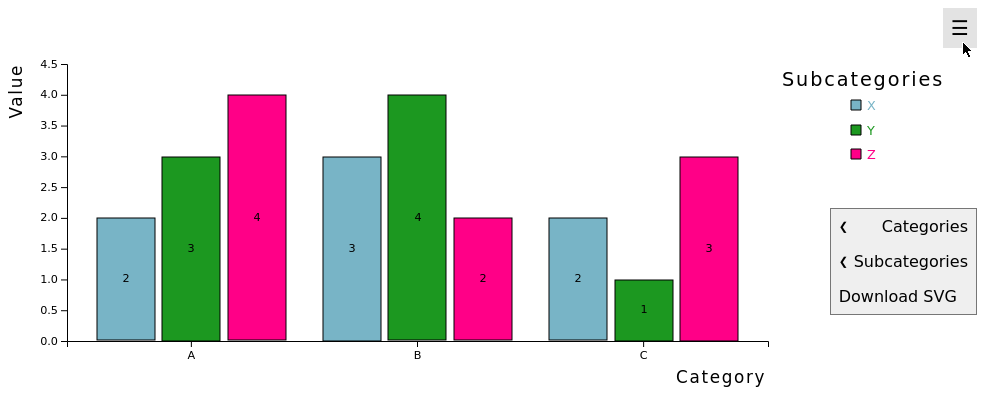
\includegraphics[keepaspectratio,width=\linewidth,height=\fullh]{images/grouped-bar-chart-window.png}
\caption[Grouped Bar Chart Window Example]{
  The resulting Grouped Bar Chart of the example code in Listing~\ref{list:GroupedBarChartWindow}. 
  The Tool Menu popup has manually been displaced to not cover the legend. 
  \imgcredit{Image created by the author of this thesis using RespVis.}
}
\label{fig:GroupedBarChartWindow}
\end{figure}

\subsection{Stacked Bars}

ein stacked bar chart wird verwendet um die relativen beitraege mehrerer quantitativer dimensionen zu einem kombinierten gesamten von unterschiedlichen kategorien eines kategorischen datensatzes miteinander zu vergleichen.
die quantitativen dimensionen koennen als unterkategorien der einzelnen kategorien gesehen werden und muessen in einer part-to-whole beziehung zueinander stehen.
Stacked Bar Charts existieren in zwei verschiedenen variationen: Basic Stacked Bar Charts und Percent Stacked Bar Charts.
bei Basic Stacked Bar Charts werden alle bars einer kategorie einfach uebereinander platziert was bedeutet dass die kombinierten gesamten unterschiedlicher kategorien miteinander verglichen werden koennen.
die laengen eines Percent Stacked Bar Charts werden hingegen nur als prozentuelle anteile eines gesamten betrachtet.
das kombinierte gesamte jeder kategorie eines solchen Charts betraegt immer genau 100\% wodurch zwar die information ueber die summe aller werte einer kategorie verloren geht aber die beitraege der einzelnen werte zu dem gesamten klarer ersichtlich ist.
alle bars innerhalb einer kategorie werden uebereinander platziert und die bars die der selben unterkategorie angehoeren haben den selben style.
das abbilden von kategorien und quantitativen werten auf raeumliche dimensionen wird so wie bei Basic Bar Charts ueber eine band scale und eine continuous scale erreicht.
der unterschied besteht darin, dass der ursprung von bars nicht auf dem unteren extrem der value scale liegt sondern sich aus der summe der laengen der vorhergegangenen bars derselben kategorie ergibt.

die RespVis library stellt drei verschiedene komponenten unterschiedlicher layer fuer das rendern von Stacked Bar Charts zur verfuegung.
die Stacked Bar Series, Stacked Bar Chart und Stacked Bar Chart Window komponenten sind ihren gegenstuecken fuer das rendern von Grouped Bar Charts sehr aehnlich.
auch bei diesen komponenten werden bars ueber die zwei-dimensionale (kategorie/unterkategorie) gruppierung von quantitativen werten gerendert, wobei eigenschaften welche individuelle bars beeinflussen ebenfalls als ein zwei-dimensionales array konfiguriert werden koennen.
der hauptunterschied in der implementierung der Stacked Bar Series von der Grouped Bar Series besteht in der berechnung der positionen und ausmasse von bars.
Stacked Bar Charts sind, so wie Grouped Bar Charts, kartesische Charts die aus einer Stacked Bar Series mit optionalen labels, zwei achsen, und einer legende bestehen.
Stacked Bar Chart Windows sind ebenfallst äquivalent zu ihren Gegenstuecken von Grouped Bar Charts und rendern einen Stacked Bar Chart innerhalb eines Layouters unter einhaltung des erforderlichen render prozesses waehrend in der toolbar tools fuer das filtern der kategorien und unterkategorien des gerenderten Charts zur verfuegung gestellt werden.
um das rendern eines Percent Stacked Bar Charts zu vereinfachen, koennen die quantitativen werte in dem datenobjekt eines Stacked Bar Chart Windows ueber die \code{valuesAsRatios} boolean eigenschaft als anteile deklariert werden was dazu fuehrt dass werte in prozentuelle anteile ihrer summen innerhalb einer kategorie transformiert werden.
in Listing~\ref{list:StackedBarChartWindow} ist der notwendige code ersichtlich mit dem ein skalierendes Stacked Bar Chart Window erzeugt werden kann dessen kategorien und unterkategorien ueber die toolbar gefiltert werden koennen.
das gerenderte resultat dieses codes kann in Figure~\ref{fig:StackedBarChartWindow} gesehen werden.


\begin{samepage}
\lstinputlisting[%
  float=tp,
  aboveskip=\floatsep,
  belowskip=\floatsep,
  xleftmargin=0cm,              % no extra margins for floats
  xrightmargin=0cm,             % no extra margins for floats
  %
  basicstyle=\footnotesize\ttfamily,
  frame=shadowbox,
  numbers=left,
  label=list:StackedBarChartWindow,
  caption={[Stacked Bar Chart Window Example]%
    The example source code that creates a Stacked Bar Chart Window.
    The Stacked Bar Chart Window is configured with the bound data object that is initialized via the \code{chartWindowBarStackedData} function.
    After configuration, the Chart Window is rendered by the \code{chartWindowBarStackedRender} function.
    Since no special responsive behavior is desired in this example, the default resize, category filter, and subcategory filter behavior is attached to the Chart Window via the \code{chartWindowBarStackedAutoResize}, \code{chartWindowBarStackedAutoFilterCategories}, and \code{chartWindowBarStackedAutoFilterSubcategories} functions. 
  },
]{listings/stacked-bar-chart-window.js}
\end{samepage}
  
\begin{figure}[tp]
\centering
\subfloat[Basic Stacked Bar Chart]{%
\hspace{1cm}
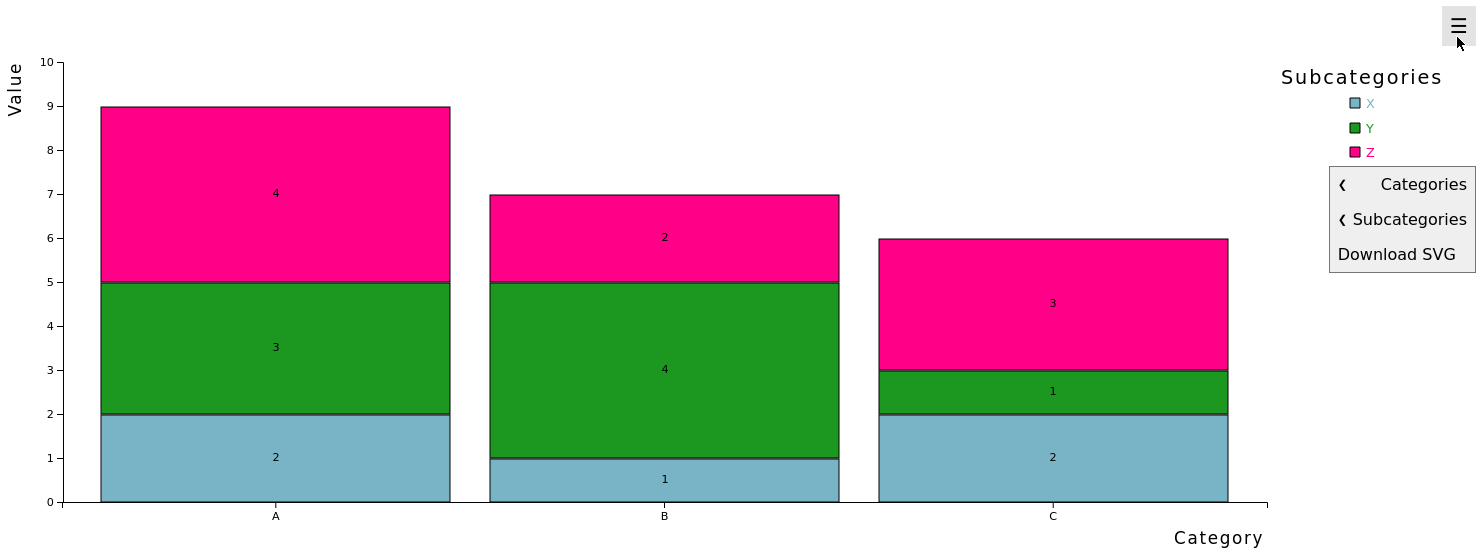
\includegraphics[keepaspectratio,width=\linewidth,height=\fullh]{images/stacked-bar-chart-window.png}
\hspace{1cm}
\label{fig:StackedBarChartWindow1}
}
\hspace{1cm}
\subfloat[Percent Stacked Bar Chart]{%
\hspace{1cm}
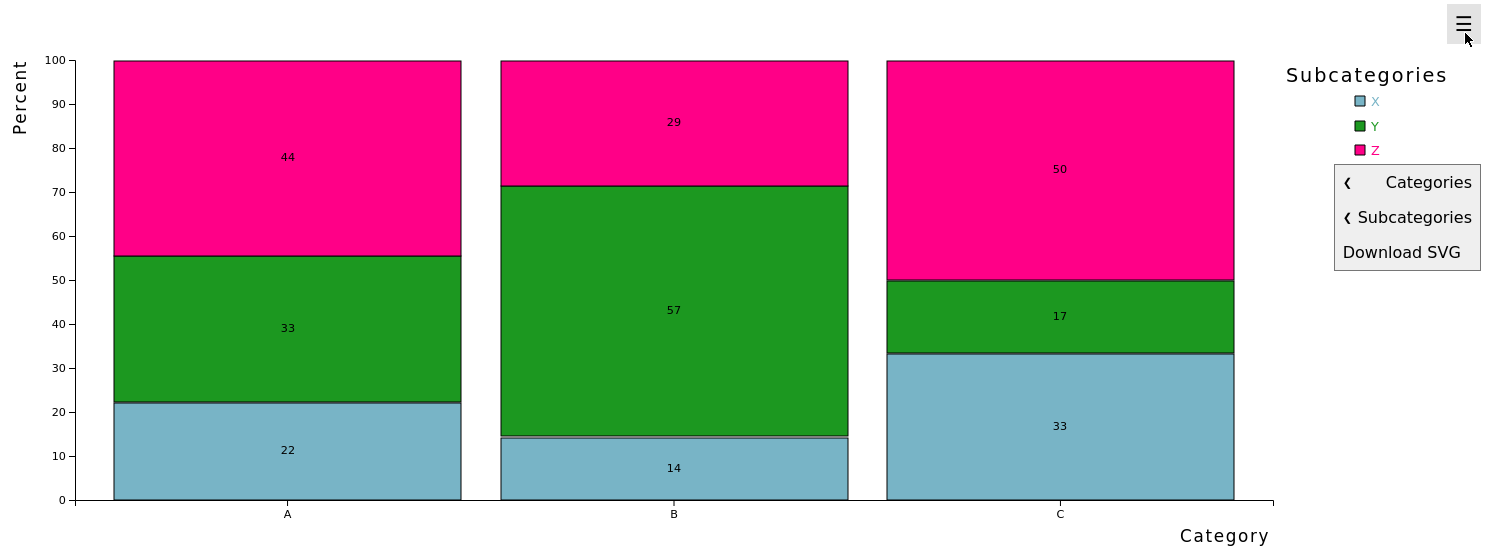
\includegraphics[keepaspectratio,width=\linewidth,height=\fullh]{images/percent-stacked-bar-chart-window.png}
\hspace{1cm}
\label{fig:StackedBarChartWindow2}
}
\caption[Stacked Bar Chart Window Example]{%
  The resulting Stacked Bar Charts of the example code in Listing~\ref{list:StackedBarChartWindow}. 
  The Tool Menu popup has manually been displaced to not cover the legend.
  \subref{fig:StackedBarChartWindow1} A Basic Stacked Bar Chart to compare the category totals and subcategory contributions to these totals.
  \subref{fig:StackedBarChartWindow2} A Percent Stacked Bar Chart to better compare the subcategory contributions to category totals. 
  \imgcredit{Image created by the author of this thesis using RespVis.}
}
\label{fig:StackedBarChartWindow}
\end{figure}
  


\section{Point Module}

Point Charts, manchmal auch scatter charts oder scatter plots genannt, werden verwendet um die beziehung zwischen zwei dimensionen eines datensatzes ueber punkte in einem kartesischen koordinatensystem zu verdeutlichen.
ueber eine solche visualisierung koennen potentielle korrelationen und muster zwischen diesen dimensionen identifiziert werden.
ueblicherweise werden zwei numerische dimensionen fuer die positionierung der punkte verwendet.
die art der zu visualisierenden daten ist jedoch nicht von bedeutung, solange individuelle werte ueber eine scale auf raeumliche dimensionen abgebildet werden koennen.
durch zusaetzliche kodierung der punkte mit farben, groessen oder formen koennen mehr als zwei dimensionen in einem Point Chart visualisiert werden.
Point Charts in welchen eine dritte dimension ueber die groesse der punkte visualisiert wird, werden auch bubble charts genannt.
der source code um einen skalierenden Point Chart mit der RespVis library zu erzeugen befindet sich in Listing~\ref{list:PointChartWindow} und die daraus resultierende visualisierung kann in Figure~\ref{fig:PointChartWindow} gesehen werden.  

\begin{samepage}
\lstinputlisting[%
  float=tp,
  aboveskip=\floatsep,
  belowskip=\floatsep,
  xleftmargin=0cm,              % no extra margins for floats
  xrightmargin=0cm,             % no extra margins for floats
  %
  basicstyle=\footnotesize\ttfamily,
  frame=shadowbox,
  numbers=left,
  label=list:PointChartWindow,
  caption={[Point Chart Window Example]%
    The example source code that creates a Point Chart Window.
    The Point Chart Window is configured with a bound data object that is initialized via the \code{chartWindowPointData} function.
    After configuration, the Chart Window is rendered by the \code{chartWindowPointRender} function.
    Since no special responsive behavior is desired in this example, the default resize behavior is attached to the Chart Window via the \code{chartWindowPointAutoResize} function. 
  },
]{listings/point-chart-window.js}
\end{samepage}
  

\begin{figure}[tp]
\centering
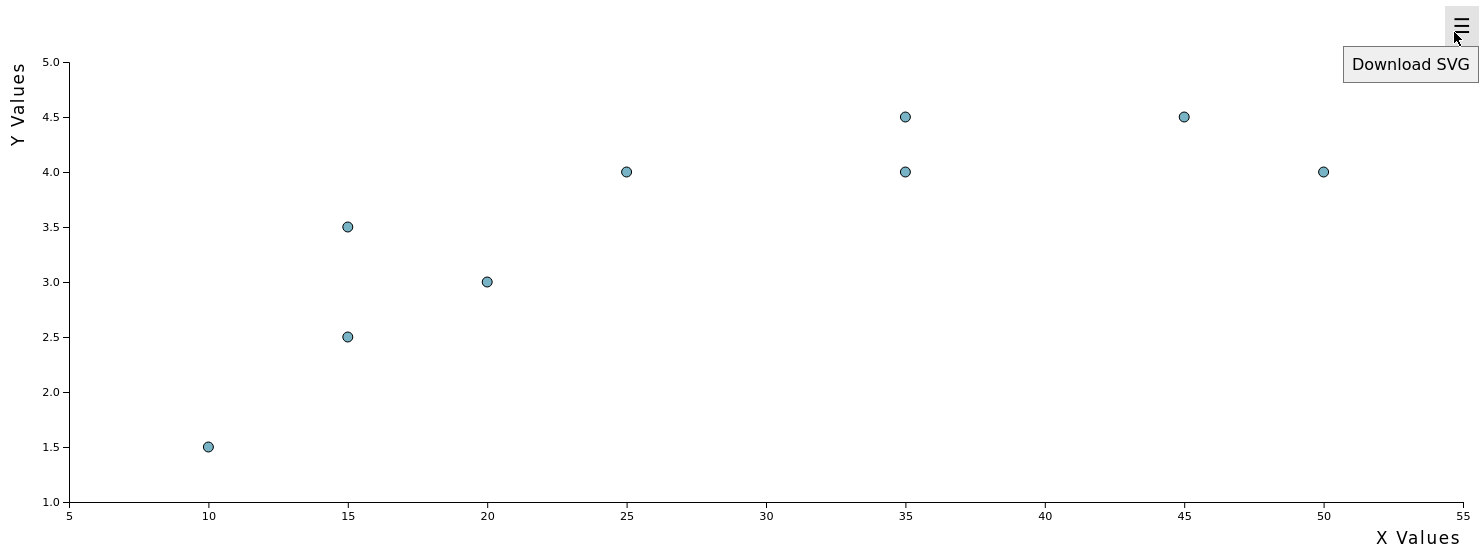
\includegraphics[keepaspectratio,width=\linewidth,height=\fullh]{images/point-chart-window.png}
\caption[Point Chart Window Example]{
  The resulting Point Chart of the example code in Listing~\ref{list:PointChartWindow}. 
  \imgcredit{Image created by the author of this thesis using RespVis.}
}
\label{fig:PointChartWindow}
\end{figure}
  

das Point Module befindet sich im \code{src/lib/point/} ordner der RespVis library und beinhaltet die implementierung der Point Series, Point Chart, und Point Chart Window komponenten.
mit einer Point Series wird eine sammlung an \code{<circle>} elementen gerendert deren mittelpunkte ueber X und Y werte arrays mit deren dazugehoerigen X und Y scales bestimmt werden und deren styles ueber style klassen gesetzt werden.
da die radiuse der einzelnen \code{<circle>} elemente konfigurierbar sind, kann eine Point Series auch verwendet werden um einen bubble chart zu erzeugen.
wie auch bei anderen Series Components, wird auch hier das gebundene datenobjekt in ein array an datenobjekten transformiert welches verwendet wird um die elemente der Series ueber einen data join zu rendern.
ein Point Chart ist ein kartesischer Chart mit einer Point Series in seiner draw area und zwei achsen welche die scales visualisieren mit welchen die Point Series gerendert wurde.
Point Chart Windows sind wrapper komponenten um Point Charts die diese in einen Layouter einbetten, ihren render prozess abwickeln, und sie mit einer toolbar dekorieren.
zum aktuellen zeitpunkt wird nur ein SVG download tool ueber die toolbar eines Point Chart Windows zur verfuegung gestellt da bislang nur eine begrenzte anzahl an tools entwickelt wurden und diese sich nicht fuer die anwendung an Point Charts eignen.
werden weitere tools benoetigt muessen diese manuell von visualisierungsauthoren implementiert und hinzugefuegt werden.     

\cleardoublepage
\chapter{Examples}
\label{chap:Examples}

\section{Bar Chart}

\section{Grouped Bar Chart}

\section{Stacked Bar Chart}

\section{Scatterplot}

\TODO{Write about application example (newspaper article?)} 

\cleardoublepage
%----------------------------------------------------------------
%
%  File    :  thesis-details.tex
%
%  Author  :  Keith Andrews, IICM, TU Graz, Austria
% 
%  Created :  17 Nov 2004
% 
%  Changed :  17 Nov 2004
% 
%----------------------------------------------------------------

\chapter{Selected Details of the Implementation
(and Test of Extremely
Long Chapter Titles to See How They Work or Not)
}

\label{chap:SelectedDetails}


\chapquote{
The devil is in the detail.
}
{
English proverb.
}


There are often specific details of a project, which involve
particularly much work to get right, but do not form a major part in
the whole scheme of things, so would not generally deserve a chapter
of their own. This chapter is for these details.



\section{First Selected Detail}

The context, the decision process, all the variations that were tried,
and the solution that was finally adopted.



\section{Second Selected Detail}

From some other part of the project. Explaining your reasoning and
choices will help some other poor student, who has to pick up your
work from where you left off.



\section{Using a Table}

An example of using a table can be seen in Table~\ref{tab:BestPubs}.

\begin{table}[tp]
\centering
\begin{tabularx}{\linewidth}{|llrX|}
\hline
Name & Type & Rating & Description \\
\hline
Flann O'Brien &
Irish &
***** &
In the centre of town and easy to find for
marauding tourists. Very smooth Guinness.
\\
\hline
The Office &
English &
***** &
Hidden in the narrow streets of the old town.
Erasmus student night every other Wednesday.
\\
\hline
O'Carolans &
Irish &
*** &
In the centre of town in a small side street next to Flann's.
Small, cosy, but hellishly smoky.
\\
\hline
O'Riginal &
pseudo Irish &
 &
Austrian dive pretending to be an Irish pub.
\\
\hline
\end{tabularx}

\caption[Best Pubs in Graz]
{
The best pubs in Graz.
}
\label{tab:BestPubs}
\end{table}





\section{Using Subfigures}

This example shows how to include vector graphics in the form of PDF
files. It also shows how to use subfigures within a figure.

\begin{figure}[tp]
\centering
\subfloat[][%  the % chars remove implicit spacing
An object has been composed to represent an
abstract version of the clock tower in Graz.
Here, the object is in its initial state.
]
{%
\includegraphics[width=0.45\linewidth]
{diagrams/multi1.pdf}%
\label{fig:Tower1}%
}
\hfill
\subfloat[][%
The object has been scaled and rotated, and now resembles
a leaning tower.
]
{%
\includegraphics[width=0.45\linewidth]
{diagrams/multi2.pdf}%
\label{fig:Tower2}%
}

\caption[Abstract Clock Towers]
{
The leaning tower of Graz. An abstract model of the clock
tower in Graz leaning over time. \subref{fig:Tower1} shows
the initial state. \subref{fig:Tower2} shows the final state.
\imgcredit{Both images created by the author of this thesis.}
}
\label{fig:WholeFig}
\end{figure}


An example of using the \vname{subfig} package can be seen in
Figure~\ref{fig:WholeFig}. Figure~\ref{fig:Tower1} shows the polygons
before transformation, while Figure~\ref{fig:Tower2} shows them
afterwards.





\section{Including a Screenshot}

This example shows how to include a screenshot (or other raster
graphic) into a \LaTeXe\ figure.

\begin{figure}[tp]
\centering
\includegraphics[keepaspectratio,width=\linewidth,height=\halfh]
{images/pist.png}

\caption[VRwave in Flip Mode]
{%
VRwave in Flip mode displaying a textured model of a cavalry pistol
from the world-renowned Zeughaus (armoury) in Graz.
\imgcredit{Image extracted from \textcite[page~81]{Andrews-VRwave}
and used under the terms of the ACM Copyright Policy. \copyrightACM}
}
\label{fig:Pistol}
\end{figure}


An example of how to correctly cite the source when using an image
from someone else. In their 1998 paper, \textcite{Andrews-VRwave}
discuss the VRwave VRML browser. Figure~\ref{fig:Pistol} shows a VRML
model of a cavalry pistol from the Armoury in Graz displayed in the
VRwave VRML browser.





\section{Using Special Characters and Symbols}

You can use many (but not all) of the thousands of characters
available in the UTF-8 \parencites{Wikipedia-UTF8}{Unicode-Charts}
character encoding. For example, the German umlauts (äüö), the German
sharp s (ß), or the yen symbol (¥).

You can also try some of the \approxsym 100 symbols available
in the \vname{textcomp} package, such as the yen symbol (\textyen) and
a circled letter A (\textcircled{A}).



\section{Using Macros to Style Special Names}

Use the \vname{vname}, \vname{cname}, and \vname{fname} macros to
define the style for (say) variable names, class names, and file
names. You can also define your own macros. The is a very long file
name \fname{/usr/data/keith/travel/austria/vienna.txt} to see how they
are broken at a line end. A typical class name is
\cname{HVSInformationPyramidsInputFactory}.





\section{Using Macros as Shorthand}

Sometimes, a macro (new command definition) can be useful to define
the contents of table cells, particularly if these contain images. For
example, Table~\ref{tab:WinIconicLang} uses the macro called
\vname{iibox}, which takes a single parameter, the name of
the particular image.


\begin{table}[tp]

\newcommand{\iibox}[1]{\parbox[c][1cm][c]{1cm}{%
\includegraphics[scale=0.6]{./images/icons/#1.png}
}}

\begin{center}
\begin{tabular}[t]{|p{7cm}c|}
\hline
\multicolumn{2}{|l|}{\sffamily \bfseries Elementary Symbols}            \\
Document                            & \iibox{win-il-gen-doc}            \\
Assistant                           & \iibox{win-il-gen-ass}            \\
Template                            & \iibox{win-il-gen-tmpl}           \\
\hline
\multicolumn{2}{|l|}{\sffamily \bfseries Document Types}                \\
Text document                       & \iibox{win-il-text-doc}           \\
Spreadsheet document                & \iibox{win-il-spreadsheet-doc}    \\
Presentation document               & \iibox{win-il-presentation-doc}   \\
Database document                   & \iibox{win-il-database-doc}       \\
\hline
\multicolumn{2}{|l|}{\sffamily \bfseries Applications}                  \\
Word                                & \iibox{win-il-word-appl}          \\
Excel                               & \iibox{win-il-xls-appl}           \\
Powerpoint                          & \iibox{win-il-ppt-appl}           \\
Access                              & \iibox{win-il-mdb-appl}           \\
\hline
\multicolumn{2}{|l|}{\sffamily \bfseries Generated Icons}               \\
Word text document                  & \iibox{win-il-word-doc}           \\
Excel spreadsheet document          & \iibox{win-il-xls-doc}            \\
Powerpoint presentation document    & \iibox{win-il-ppt-doc}            \\
Access database document            & \iibox{win-il-mdb-doc}            \\[2ex]
%
Word template                       & \iibox{win-il-word-tmpl}          \\
Powerpoint template                 & \iibox{win-il-ppt-tmpl}           \\
Access template                     & \iibox{win-il-mdb-tmpl}           \\[2ex]
%
Word template assistant             & \iibox{win-il-word-ass}           \\
Powerpoint template assistant       & \iibox{win-il-ppt-ass}            \\
Access template assistant           & \iibox{win-il-mdb-ass}            \\[2ex]
%
\hline
\end{tabular}
\end{center}

\caption[Iconic language for Windows NT 4.0 documents]
{
Iconic language for Windows NT 4.0 documents.
\imgcredit{The icons are screenshots, captured and then
enlarged by the author of this thesis.}
}
\label{tab:WinIconicLang}
\end{table}







\begin{samepage}
\begin{lstlisting}[%
  float=tp,
  aboveskip=\floatsep,
  belowskip=\floatsep,
  xleftmargin=0cm,              % no extra margins for floats
  xrightmargin=0cm,             % no extra margins for floats
  basicstyle=\footnotesize\ttfamily,
  frame=shadowbox,
  numbers=left,
  language=HTML,
  label=list:HTML5Boilerplate,
  caption={[HTML5 Boilerplate Code]%
Some HTML5 boilerplate code, illustrating the typical structure
of a HTML5 web page.
},
]
<!DOCTYPE html>
<html xmlns="http://www.w3.org/1999/xhtml" lang="en" xml:lang="en">

<head>
<meta charset="UTF-8"/>
<meta name="viewport" content="width=device-width, initial-scale=1"/>
<link rel="stylesheet" href="./inm.css"/>

<title>Keith Andrews Web Page</title>
</head>

<body>

<header>
<img src="images/kalogo.svg" alt="KA Logo"/>
Keith Andrews Design
</header>

<h1>Keith Andrews</h1>

<p>
Keith lives in <a href="http://graz.at/">Graz</a>.
</p>

<p>
<img src="images/keith-s.jpg"
  alt="Photo of Keith Andrews"/>
</p>

<p>
Three desirable attributes:
</p>
<ol>
<li>cheap</li>
<li>fast</li>
<li>good</li>
</ol>
<p>
Choose any two.
</p>

<p>
<abbr title="Extensible HyperText Markup Language">XHTML</abbr>
is cool.
</p>

<table>
<tbody>
<tr><th>Beer</th><th>Price €</th></tr>
<tr><td>Puntigamer</td><td>2,60</td></tr>
<tr><td>Gösser</td><td>2,60</td></tr>
<tr><td>Guinness</td><td>4,35</td></tr>
</tbody>
</table>

<footer>
Copyright © Keith Andrews 2019.
</footer>

</body>
</html>
\end{lstlisting}
\end{samepage}



\section{Using Floating Listings}

Listing~\ref{list:HTML5Boilerplate} is floating. A floating listing is
a block of code treated like other \LaTeXe floats (such as figures or
tables). Use floating listings for longer blocks of code.
A floating listing is given a number and can be referred to
explicitly, like Listing~\ref{list:HTML5Boilerplate}. It can be given
a caption and short caption, and is listed in the List of Listings.





\section{Using Non-Floating Diplayed Listings}

The listing below shows some CSS:
\begin{samepage}
\begin{lstlisting}[%
  language=CSS,
]
body { color: black; background-color: silver; }
img { border: none; }
h1,h2 { font-family: Verdana, sans-serif; }
\end{lstlisting}
\end{samepage}
It is displayed (i.e. indented as a block) in-place, but is not
floating. It cannot be referred to by number and is not listed in the
List of Listings. As a rule of thumb, if listings have five or more
lines, make them floating.





\section{Using Inline Listings}

Inline listings are used for very short snippets of code embedded
within the flow of a paragraph. For example,
\lstinline|\lstinline!var i:integer;!|
produces
\lstinline!var i:integer;!, which can now be discussed further.
Do not break an inline listing over multiple lines (EOL).




\section{Using Lists}

A list should always be introduced by a sentence
which ends with a colon.
%
There are three kinds of standard lists in \LaTeXe:
\begin{itemize}
\item itemize
\item enumerate
\item description
\end{itemize}
% A blank line here would indicate a new (indented) paragraph
An enumerated list has numbered items:
\begin{enumerate}
\item Fast
\item Good
\item Cheap
\end{enumerate}
Choose any two!


A description list has named items with corresponding
definitions or descriptions:
\begin{description}
\item[Short] Each item has a label (name) and its description.

\item[Rather longer label] By default, if the description text
  is rather long, it will warp around to the following lines.
\end{description}



     

\cleardoublepage
\chapter{Outlook and Future Work}
\label{chap:Outlook}

Many things could still be done to the RespVis library that would not
change its core mechanisms, but would improve both the visualization
consumer's and visualization author's experience. One of the most
apparent improvements would be the addition of further Series, Charts,
and Chart Windows to extend the range of realizable visualizations and
enable the creation of things like parallel coordinates, pie charts,
heatmaps, small multiples, and other charts. In addition to supporting
more types of charts, the RespVis library would benefit from
additional tools which could be added to the Toolbars of Chart Windows
to provide easy access to supplementary operations like interval-based
numerical filtering and zooming. The improvements that could be made
to already existing functionality include improving interactions via
the application of Delaunay triangulation
\parencite{Delaunay,DelaunayAlgorithms} to find the closest
interactable element to the cursor position, improving downloaded SVGs
through optimizing and formatting their document contents, and
improving responsive styling via the application of the newly proposed
CSS Container Queries \parencite{CSSContainment3} when they become
available in browsers.

The layouting of SVG elements could be improved by separating
visualizations into different <div> elements that can be natively laid
out by browsers. With such a layouting mechanism, the custom Layouter
could be removed, and the render process imposed by it, which
effectively forces every laid out element to be rendered twice, would
be unnecessary. The elimination of the custom Layouter and its render
process would improve performance and be much less complex to
implement and understand. The downside of this change would be that
visualizations are not directly rendered as pure and complete SVG
documents anymore, but rather as multiple SVG documents representing
separate parts of the visualization. This separation into multiple SVG
documents would not be a problem for displaying visualizations in
browsers. To download such a visualization, its individual parts could
be merged back into a pure and complete SVG document during an
additional download pre-processing step.

Custom visualizations are rather tedious to create with the current
implementation, because visualization authors must manually set up
their structure, propagate data through the component hierarchy, and
handle the Layouter's render process. The creation of custom
visualizations could be simplified by introducing generic Chart
Windows that would enable the definition of visualizations using a
data structure potentially similar to visualization grammars like Vega
\parencite{Vega}.
% KA TODO or Cicero or Vega-Lite ??
The data structure of generic Chart Windows would have to include the
actual abstract data that should be visualized and define the
transformations of this data into scales, Axes, Legends, and Series.
During rendering, the render functions of such generic Chart Windows
could then create custom visualizations to reflect the configuration
stored in these data structures. In addition to simplifying the
creation of custom visualizations, generic Chart Windows would also
enable responsively changing a visualization's encoding, like, for
example, turning Point Charts into Heatmap Charts.


% KA TODO  small multiples?



        

\cleardoublepage
\chapter{Concluding Remarks}
\label{chap:Concl}

After giving an overview of related web technologies and the research related to the academic fields of information visualizations and responsive visualizations, this thesis introduced RespVis, a new open-source software library to create responsive visualizations for the web.
RespVis has been designed as an extension of the D3 library and renders visualizations as SVG documents styled with CSS.
The most novel contribution of this work is a custom layouter that uses the browser's own layout engine to enable visualization authors to configure the layout of SVG-based visualization components via CSS.
Since rearranging content is one of the main techniques of responsive web design, enabling visualization authors to use CSS layout mechanisms like Flexbox and Grid to reposition visualization components leads to much better responsive capabilities than merely allowing them to change their styles.
Relying on CSS for a large amount of a visualization's configuration also leads to visualization authors benefitting from being able to utilize CSS media queries for responsive styling and from the simplicity of using a tool they are already familiar with.
Furthermore, since RespVis' API is mostly meant for configuring a visualization's content and behavior, it can be much more minimal than it would be if the complete style of a visualization would also be configured via it.
This minimal API and RespVis' reliance on standards like SVG and CSS for rendering and configuring its visualizations result in much less likelihood that visualization authors are limited by API restrictions.
Due to all of these reasons, it is evident that RespVis has the potential to be a very effective library for the creation of responsive visualizations after some more improvements are made to it.
       

\appendix

\cleardoublepage
%----------------------------------------------------------------
%
%  File    :  thesis-user.tex
%
%  Author  :  Keith Andrews, ISDS, Graz University of Technology
% 
%  Created :  27 Jan 2019
% 
%  Changed :  27 Jan 2019
% 
%----------------------------------------------------------------

\chapter{User Guide}

\label{app:UserGuide}

A thesis in computer science will often involve the writing of
software. In such cases, it is common to have a user guide and
sometimes also a developer guide as appendices.
The user guide is aimed at end users of the software.
It typically covers the following aspects:
\begin{itemize}
\item \liintro{Installation}: a description of how to install the
  software.

\item \liintro{Features}: an overview of what the software can do.

\item \liintro{User Interface}: a thorough tour of elements of the
  user interface, their purpose, and how to use them, illustrated with
  numerous screenshots.

\item \liintro{Usage}: a series of ``recipes'' explaining how to
  accomplish common tasks.

\item \liintro{FAQs}: answers to a number of (anticipated) frequently
  asked questions.
\end{itemize}
The user guide should be a stand-alone document, complete in itself,
even if that requires some duplication with material or screenshots
contained within the main thesis.


           % Appendix A

\cleardoublepage
%----------------------------------------------------------------
%
%  File    :  thesis-developer.tex
%
%  Author  :  Keith Andrews, ISDS, Graz University of Technology
% 
%  Created :  27 Jan 2019
% 
%  Changed :  27 Jan 2019
% 
%----------------------------------------------------------------


\chapter{Developer Guide}
\label{app:DeveloperGuide}

The developer guide is aimed at fellow developers, who might modify or
extend the software in future. It typically covers some or all of the
following aspects:
\begin{itemize}
\item Development environment and tools.

\item Software dependencies.

\item APIs.

\item Mechanisms for extensions, such as hooks or plugins.

\item How to integrate a new piece of code, such as an
  alternative search algorithm or visualisation.
\end{itemize}



      % Appendix B



\backmatter

% Ensure that certain references are listed in the bibliography,
% even if they are not cited anywhere in the text.
% \nocite{KeithMastersThesis}
% \nocite{KeithPhdThesis}


\cleardoublepage
% for now, switch to language english
% hack to force unix date for biblio, biblatex 3.11
\begin{otherlanguage}{english}
  \printbibliography[heading=bibintoc]
\end{otherlanguage}



% \cleardoublepage
% \input{glossary}      % Glossary

% \cleardoublepage
% \input{index}         % Index

\end{document}

